\documentclass[12pt]{article}
\usepackage{graphicx} % Required for inserting images
\usepackage{float}
\usepackage{geometry}
\usepackage{natbib} 
\usepackage{hyperref}
\usepackage{xcolor}

\graphicspath{ {/home/gonzalopc/Documentos/programas_mios/TFM_AFI_2025/TFM_AFI_2025/mynotes/images/} }

\setlength{\parskip}{4mm}
\textwidth 15cm
\leftmargin 2cm
\rightmargin 1cm
\setlength{\baselineskip}{18pt}

%Transporte marítimo e incautación de droga
% 

\title{\bf AFI - Global Education\\
\vspace{3cm}
Máster Executive en Data Science, Big Data e Inteligencia Artificial\\
\vspace{2cm}
\begin{center}
	\hspace*{0cm}
	
\includegraphics[width=0.4\textwidth]{afi_logo.png} \\
\end{center}

\vspace{2cm}
Trabajo Fin de Máster\\
\vspace{1cm}
Transporte marítimo e incautación de droga
}

\author{
		\bf Autor: Gonzalo López Segovia \\
		\bf Tutor: José Manuel Rodríguez
	}                                                                                            
\date{\bf Marzo 2025}


% Keywords command
\providecommand{\keywords}[1]
{
	\small	
	\textbf{\textit{Keywords---}} #1
}

\geometry{
	a4paper,
	total={170mm,257mm},
	left=20mm,
	top=20mm,
}

%\renewcommand{\baselinesetstretch}{1.25}

\begin{document}
	
	%Incluir Logo AFI en la Portada

	
%\Large

\maketitle

\newpage

\tableofcontents

\newpage

\listoffigures

\newpage

\listoftables

\newpage

\section{\label{resumen}Resumen}
El transporte marítimo es parte esencial del comercio internacional. No obstante, también es un canal de entrada principal para las redes de narcotráfico internacionales. En este estudio, se analiza el volumen de actividad en distintos puertos comerciales en Estados Unidos, medido en tráfico de contenedores, y la cantidad de droga incautada por las oficinas de campo del servicio de aduanas de Estados Unidos para las áreas metropolitanas próximas a esos puertos. También se busca hallar una posible relación entre estos dos conceptos. Para ello, se ha hecho uso de distintas técnicas de Machine Learning aprendidas desde modelos de regresión a modelos de series temporales. Los resultados muestran patrones de incautaciones que varían según la ubicación y el tipo de droga. Sin embargo, la correlación directa con la actividad portuaria se verá que no es concluyente y afectará en el desarrollo y desempeño de los distintos modelos de predicción. A pesar de las limitaciones en los datos disponibles y en la sobrevaloración en la concepción misma del trabajo, éste mismo ofrece una base para mejorar la detección de tráfico ilícito a través de un buen análisis y optimizar la gestión de recursos.

\section{\label{abstract}Abstract}
Maritime transport is an essential part of international trade. However, it is also a major entry channel for international drug trafficking networks. This study analyzes the volume of activity in various commercial ports in the United States, measured in container traffic, and the amount of drugs seized by the U.S. Customs Field Offices in metropolitan areas near these ports. It also aims to identify a possible relationship between these two factors. To achieve this, various Machine Learning techniques have been applied, ranging from regression models to time series models. The results show seizure patterns that vary depending on location and drug type. However, the direct correlation with port activity is found to be inconclusive, impacting the development and performance of the different predictive models. Despite the limitations in the available data and the overestimation in the initial conception of the study, this research provides a foundation for improving illicit trafficking detection through thorough analysis and optimizing resource management.

\keywords{Transporte marítimo, Geografía del Transporte, Geografía Marítima, Drogas, Estupefacientes, Narcotráfico, Machine Learning, Análisis de Datos, Clustering}

\newpage
% Añadir indice de contenidos

\section{\label{intro}Introducción}
	El transporte marítimo ha sido, desde la Antigüedad, el eje central del comercio global. Imperios y civilizaciones han dependido de rutas marítimas para el intercambio de bienes, desde las redes comerciales del Mediterráneo hasta las rutas coloniales que unieron continentes en la era moderna. Sin embargo, fue la Revolución Industrial la que transformó radicalmente la logística marítima, con avances avances en la construcción naval y, más recientemente, con la revolución de la contenerización iniciada en 1956 por el Ideal-X en su ruta Newark-Houston (\cite{wired2012container}). Este cambio permitió una drástica reducción en los tiempos y costos de carga y descarga, consolidando el transporte de contenedores como el estándar del comercio global. Hoy en día, la mayor parte del comercio internacional depende de esta infraestructura, con puertos como Los Ángeles, Shanghái y Rotterdam actuando como nodos críticos de la economía mundial.
	
	No obstante, la misma eficiencia y globalización que han impulsado el comercio legal, también han facilitado el tráfico de productos ilegales, especialmente de drogas. Los puertos marítimos, debido a su alto volumen de carga y complejidad logística, representan un punto vulnerable para el contrabando de sustancias ilícitas. Aprovechando las rutas comerciales establecidas y las infraestructuras portuarias, es posible ocultar cargamentos de drogas entre mercancías legítimas, desafiando los sistemas de inspección y control aduanero. Este fenómeno no es reciente: desde las Guerras del Opio en el siglo XIX hasta la actual crisis de opiáceos, el narcotráfico ha estado intrínsecamente ligado a las dinámicas del comercio global.
	
	Estados Unidos, como principal mercado de consumo, y China, como fuente de precursores químicos (\cite{justice2023indictments} y \cite{justice2023fentanyl}), ejemplifican la interconexión entre el comercio legal e ilegal en la actualidad. Los flujos comerciales reflejan no sólo la globalización económica, sino también la propagación de bienes de consumo ilícitos a través de las mismas infraestructuras que sustentan el comercio mundial. En este contexto, el estudio del tráfico marítimo y la incautación de droga en puertos se vuelve crucial para comprender los patrones delictivos y fortalecer las estrategias de detección y control.
	
	Este trabajo explorará la relación entre el comercio marítimo y el tráfico de drogas, analizando datos sobre el movimiento de contenedores y las incautaciones realizadas en los principales puertos de EE.UU. a partir de registros oficiales del CBP (\cite{cbp_website}). A través de un enfoque basado en datos, se intentará identificar, si fuera posible, patrones geográficos, de tendencias temporales o si existiese la correlación entre el volumen de contenedores manejados por cada puerto y la cantidad de incautaciones reportadas por sus correspondientes "oficinas de campo" (o Field Office en su versión original) del CBP.
	
	El objetivo de este trabajo es intentar aportar una visión cuantitativa sobre cómo el tráfico marítimo y las operaciones de control en los puertos de EE.UU. interactúan en el contexto del narcotráfico, pudiendo proporcionar información valiosa para mejorar las estrategias de detección y prevención.
	
	

	\subsection{\label{antecedentes}Antecedentes}
	Importancia del transporte marítimo en el comercio global:
	\begin{description}
		\item[-] Según el documento de la OECD (An Ocean of Data) más del 80\% del comercio global en volumen y el 70\% en valor se transporta por vía marítima (\cite{pilgrim2024ocean}).
		\item[-] Los puertos son nodos críticos para la economía mundial, funcionando como infraestructuras de interconexión entre lo local y lo global.
		\item[-] Las nuevas tecnologías, como los sistemas AIS (\cite{nauticaprofesional2025ais}), han permitido un mejor rendimiento de la actividad portuaria y del tráfico comercial, lo que facilita el análisis de patrones comerciales y posibles interrupciones.
		\item[-] En 2019, el volumen total de mercancías transportadas por mar superó los 11.000 millones de toneladas métricas. \cite{cidob2025maritime}
	\end{description}
	
	Relación con el tráfico de drogas:
	\begin{description}
		\item[-] A partir del trabajo realizado por Coufal para la Universidad de Amsterdam (\cite{coufal2023cities}) para los puertos de Roterdam y Amberes se intentará realizar un análisis para los puertos de EE.UU.
		\item[-] La enorme cantidad de contenedores que llegan diariamente dificulta la detección de cargamentos ilícitos, lo que convierte a estos puertos en objetivos estratégicos para el crimen organizado.
	\end{description}

	En definitiva, las investigaciones previas en los que se basa este tabajo sirven para mostrar como el crecimiento del comercio marítimo junto con la voluminosa gestión de cargamento dificulta la detección de estupefacientes y, a su vez, facilita su introducción en mercados de alto consumo a través de los mismos.
	
	\subsection{\label{motivacion}Motivación del proyecto}
	% Descripción del problema
	El origen de este proyecto se basa principalmente en el interés de aplicar los conocimientos sobre la geografía humana a nivel del comercio internacional. Esto junto con informaciones de interés relacionado con ciertas actividades ilícitas que se dan en zonas portuarias, dio paso a intentar averiguar si se podía estimar la cantidad de droga que entraba en un puerto cualquiera a partir del trasiego de contenedores en un puerto comercial. Pese a que en un principio se intentó realizar para la vía comercial del Pacífico exclusivamente y basándose en el flujo de barcos cargueros entre estas regiones, las dificultades a la hora de obtener datos de fuentes privadas (como la necesidad de obtener una licencia para explotar los datos), hizo desde muy pronto bajar las expectativas y reformular el punto de partida.
	
	Las fuentes privadas orientadas a la explotación de los datos a nivel empresarial, facilitan un enfoque para cualquiera de estas empresas relacionadas con el comercio, los procesos logístico o la especulación financiera. Los datos abiertos, con un enfoque de más información transparente sobre resultados de administraciones, podrían en parte suplir las carencias de no poder acceder a las fuentes privadas. Es por ello que el problema se reorienta desde un punto de vista del transporte de mercancías por flujo de barcos al del trasiego de contenedores gestionado por la autoridad portuaria pertinente.
	
	Y como se venía diciendo, la motivación original de este proyecto era ir un paso más allá, intentar averiguar el flujo de entrada de droga a partir de datos de incautaciones. Sin embargo, como se verá a lo largo de este trabajo, quedará demostrado que con los datos aportados no es suficiente para predecir esta presunta conexión. Al ceñirse a actividades de éxito de las agencias de aduanas se encontrarán una serie de impedimentos:
	
	\begin{description}
		\item[1.] Pese a centrarse en actividades en puertos y fronteras, la cantidad estimada de contenedores que se investigan son apenas un 5 por ciento de los contenedores totales que pasan a diario (\cite{rodrigue2024geography}).
		\item[2.] No solo eso, los hubs portuarios se sitúan en las conocidas como ciudades globales (\cite{rodrigue2024geography}) de gran importancia económica, con gran intermodalidad entre distintos medios de transporte y capaz de conectar vías de alta capacidad, por lo que el nivel de alcance se hace demasiado extenso para poder incautar toda la droga que entra.
		\item[3.] La forma de abordar el problema relacionado con el narcotráfico a distintos niveles administrativos, junto con la legalidad de ciertas sustancias, hace que el problema no solo dependa de la cantidad que llega (la demanda) sino de la aproximación a nivel político: si se es más laxo en términos de vigilancia con cierta sustancia o, por el contrario, más estricto.
	\end{description}
	
	Esto, como se verá más adelante en \ref{Diseño}, impedirá realizar un buen análisis a partir de los datos tratados.
	
	Gran parte del origen del trabajo surge a partir del interés por la Geografía Económica y del Transporte. Trabajos como el publicado por Jean-Paul Rodrigue en \cite{rodrigue2024geography} ha servido, a pesar de todo, como acicate para aunar y profundizar conocimientos en este campo y aplicarlo a una temática sensible como es el tráfico de estupefacientes. A partir de los datos recopilados, se intentó que de algún modo u otro se pudiera si no responder, al menos plantear de forma clara la siguiente conjetura: Si conocemos la actividad económica en un puerto -entendida como trasiego de contenedores-, ¿sería posible, solo con esa información, estimar el volumen de incautación de droga para ese mismo puerto? Se deja la ventana abierta a que se trate de una droga en particular, que sea el número de redadas o que sea la cantidad (kilogramos o libras) y que sea para un puerto en exclusiva o si se pudiere generalizar a varios puertos.
	 
	\subsection{Objetivos}
	De acuerdo con los expuesto en la sección "Motivación del proyecto", este trabajo se va a encargar de:
	
	\begin{description}
		\item[1] Agrupar puertos en regiones geográficas y metropolitanas próximas denominadas "hubs portuarios" a partir de señales de comunicaciones enviadas desde barcos próximos.
		\item[2] Mostrar el comportamiento de distintos puertos con respecto al volumen de droga incautada por tipo de droga.
		\item[3] Estudiar si el comportamiento puede ser caracterizado por factores periódicos en forma de serie temporal para un intervalo de 75 meses (6 años y 1 trimestre).
		\item[4] Determinar si a partir de la actividad en un puerto comercial, dado volumen de carga y descarga en ese puerto, se podría estimar la cantidad de droga incautada en ese mismo puerto.
	\end{description}

	\subsection{Enfoque y Metodología general}
	Para la realización de este proyecto, a nivel técnico, se necesita tener conocimientos sobre estadística descriptiva, series temporales, clustering, visualización de datos, y algoritmos de aprendizaje automático (Machine Learning), especialmente en árboles de decisión y métodos de bagging y boosting. Por otro lado, para entender el origen e integración de los datos ha habido que comprender cuestiones relacionadas con la navegación marina, la gestión de bienes y recursos en puertos, así como conocer como operan las agencias de aduanas de los Estados Unidos.

	\subsection{Estructura del Documento}
	Este trabajo se divide en: una introducción donde se exponen los antecedentes, motivaciones y objetivos; una sección sobre el Estado del Arte tanto a nivel de técnicas y algoritmos de Machine Learning como conocimientos relacionados con el objetivo del problema (que sea capaz de relacionar los conocimientos sobre la geografía del transporte con las dinámicas del narcotráfico); otra sección sobre la metodología empleada en la que se detalla largo y tendido tanto el tratamiento de los datos como planteamiento del modelo que emularía el problema; otra sección "Diseño del Modelo" con los algoritmos aplicados, la implementación y la evaluación del rendimiento. Para terminar con las secciones sobre la interpretación (y visualización de los resultados) y conclusiones y trabajos futuros.

\newpage

\section{Estado del arte}
En esta sección se van a exponer las principales herramientas y conocimientos demandados para poner en marcha la realización del problema. Esta sección se subdivide en conocimientos a nivel de ciencias sociales (\ref{literatura}) con conocimientos técnicos de Machine Learning (\ref{conocimientosml}).

Por otro lado, como se comentó en \ref{motivacion}, al faltar datos de flujos y vías marítimas, no era trivial hallar la red o grafo mundial de conexiones portuarias y se reorientó a realizar un estudio in situ para cada puerto. Por último, tras enunciar las distintas herramientas y tecnologías para implementar el modelo, se han justificado el uso de estas en sus entornos de desarrollo para problemas de ciencia de datos.

	\subsection{\label{literatura}Literatura sobre el problema}
	Para el desarrollo del modelo se ha intentado que, a nivel de técnicas de Machine Learning, las soluciones propuestas estuviesen integradas en librerías de python como scikit-learn o prophet, para facilitar y acelerar su implementación. También se ha leído algo de bibliografía relacionada con el alcance del problema. Así pues, libros y estudios sobre la geografía del transporte como informes sobre las dinámicas del narcotráfico a nivel global han servido para intentar guiar el trabajo realizado. 
	
		\subsubsection{Estudio de la Geografía del Transporte.}
		% Los puertos más transitados de Estados Unidos de América.
		De acuerdo con las principales ideas de \cite{rodrigue2024geography}, la geografía del transporte se encarga de estudiar la movilidad de bienes, personas e información en el espacio geográfico con el objetivo de comprender la relación entre los sistemas de transporte y el desarrollo económico y la organización espacial, entre otros.
		
		Los avances en el transporte marítimo, tales como la contenerización, han incrementado la gestión de los cargamentos y reducido los tiempos y costos. Esta mejora viene aparejada con un aumento de la demanda del transporte, la capacidad operativa de los puertos y las dinámicas del comercio global.
		
		Pese a que el transporte marítimo representa más del 80\% del comercio global en volumen, se estima que solo entre el 2\% y el 5\% de los contenedores son inspeccionados manualmente, lo que complica su detección y facilita las oportunidades para el contrabando.
		
		En términos de tráfico, los puertos más importantes a nivel mundial se concentran en el Este Asiático, Norteamérica y Europa. Para este trabajo nos vamos a centrar en los principales puertos de Estados Unidos.
		
		
		\subsubsection{Estudio sobre dinámicas del narcotráfico}
		El tráfico de drogas a través de los puertos marítimos se ha convertido en un fenómeno complejo y en constante evolución, impulsado por la globalización del comercio y el desarrollo de redes criminales transnacionales. Estudios recientes han analizado las estrategias utilizadas por las organizaciones criminales para infiltrar cargamentos ilícitos en el comercio marítimo y las respuestas adoptadas por las autoridades para contrarrestar estas prácticas \cite{coufal2023cities}, \cite{serra2023drugsmuggling}.
		
		Uno de los principales hallazgos en la literatura es la importancia de los puertos como puntos críticos en la logística del narcotráfico. Puertos como Róterdam y Amberes se han consolidado como centros clave para la entrada de cocaína en Europa, debido a su alto volumen de tráfico, su infraestructura eficiente y su ubicación estratégica \cite{coufal2023cities}.
		
		El análisis de estas dinámicas resulta fundamental para comprender los mecanismos utilizados por el narcotráfico y evaluar la eficacia de las estrategias de control implementadas en los principales puertos del mundo. En el caso de Estados Unidos, el estudio de la relación entre el tráfico de contenedores y las incautaciones de droga permitirá identificar patrones relevantes y posibles puntos de vulnerabilidad en el sistema portuario.


	\subsection{\label{conocimientosml}Conocimiento de técnicas de Machine Learning}
	El análisis del tráfico marítimo y la detección de actividades ilícitas, como el tráfico de drogas, han sido históricamente abordados mediante métodos tradicionales basados en reglas, estadísticas descriptivas y técnicas de minería de datos convencionales (\cite{article_ortiz} y \cite{Kretschmann2020}). Los enfoques efectuados entonces presentaban determinadas carencias como son el alto grado de supervisión humana, la dificultad para detectar patrones ocultos y su escalabilidad limitada.
	Por contra, los enfoques basados en técnicas y conocimientos de Machine Learning y Data Science ofrecen una mayor capacidad de análisis, permitiendo encontrar patrones complejos, anticiparse mediante el análisis predictivo o detectar anomalías entre otros.
	
	En estudios previos sobre el tráfico marítimo y la detección de actividades ilícitas, se han utilizado diversos modelos y técnicas de Machine Learning entre los cuales, algunos de ellos serán utilizados a lo largo de este trabajo.
	
		\subsubsection{Algoritmos para métodos de regresión}
		En el contexto de este estudio, se van a emplear algoritmos de Machine Learning enfocados en la predicción a partir de datos históricos. Puesto que en este caso, uno de los propósitos es resolver un problema de regresión, se ha decidido realizar pruebas con modelos basados en árboles de decisión y técnicas, tanto de boosting como de bagging. Los algoritmos considerados candidatos vendrían a ser:
		
		\begin{description}
			\item[·] Árboles de Decisión: cuenta con la ventaja de ser interpretable y basarse en reglas. Sin embargo, las alternativas que complejizan este sencillo algoritmo tales como los métodos de bagging o boosting, dan poco margen a este tipo de algoritmos.
			\item[·] Regresión Lineal.
			\item[·] Adaboost: técnica de boosting a partir de árboles muy sencillos (modelos débiles) asignando mayor peso a los datos peor predichos.
			\item[·] Bagging: conjunto de múltiples árboles compuesto por el subconjunto aleatorio de observaciones.
			\item[·] GradientBoost: Algoritmo de boosting con librería de python propia. Su función de pérdida es diferenciable.
		\end{description}


		\subsubsection{\label{prophet}Series temporales con Prophet}
		Puesto que uno de los objetivos originales del problema era, en caso de que fuera posible, hallar la cantidad de droga incautada -con independencia del tipo- a partir de una serie temporal sobre la llegada de cargamentos, se planteó el enfoque del problema desde la caracterización de la señal por medio de series temporales.No obstante, dada, posiblemente, la falta de horizonte temporal, o ciertas características que pudieran condicionarla como una serie temporal (\cite{towardsdatascience2025timeseries}) dificultó la correcta realización de un problema de esta índole. Sin embargo, en algún caso que si se demostró factible se hizo uso de la librería prophet de Meta (\cite{Taylor2017}) para la resolución de series temporales.
		
		Para una serie temporal hay que considerar su tendencia a nivel general, si tienen comportamientos estacionales y el resto que no pudiere ser caracterizado, identificarlo como ruido blanco gaussiano (el residuo) \cite{towardsdatascience2025timeseries}.
		
		% Incluir alguna imagen de ejemplo de como tratar una serie temporal

		\subsubsection{\label{clustering}Técnicas de clustering}
	%	 Incluir Vectorial K-Means (*)\
		Como se irá viendo a lo largo del trabajo, una de las dificultades en su origen fue conectar los datos de distintos orígenes y temáticas. Por un lado, dada la gran disparidad entre el número de puertos y el número de oficinas aduaneras del CBP, se estimó necesario la agrupación de los primeros en "hubs portuarios". Para ello se barajaron distintas técnicas de clustering para poder agrupar las señales emitidas por aquellos barcos de tipo carguero (cargo ship) que se encontrasen de algún modo atracados a lo largo de una serie de días de septiembre de 2024. A partir de las señales de los barcos, se aplicó un algoritmo K-Means sencillo -tomando como variables la latitud y la longitud- para hallar aquellos puntos cercanos al litoral que mejor agrupasen barcos (y, en definitiva, puertos) cercanos entre sí.
		
		Para este problema, se utilizó 'silhouette' para medir la calidad del clustering, en detrimento de otras opciones (wss). Las ventajas de usar 'silhouette' como medida de discriminación de elementos particulares frente a clusters se encuentra en que es más robusto para clusters con distinta densidad y tiene en cuenta la separación entre clusters. También se estimó el uso de alternativas como K-Means Vectorial (\cite{ferreira2012vectorfieldkmeansclustering}), pero debido a su alcance más de nicho (no implementado en scikit-learn o cualquier otra gran librería de Python) frenó sus posibilidades de implementación, junto con la poca claridad del objetivo final del problema por aquel entonces.	
	
	\subsection{Justificación de las herramientas y tecnologías elegidas}
	Para el desarrollo de este problema de ciencia de datos, se ha hecho uso, principalmente, del lenguaje de programación python y librerías básicas asociadas al estudio de problemas de ciencia de datos, tales como pandas o scikit-learn (\cite{scikit-learn}). En algunos desarrollos se echó mano de Google Colab y otros de VisualStudio en función de si se requería una gran capacidad de recursos y cálculo. Debido a los cambios constantes en los planteamientos y objetivos del problema a causa de las dificultades inherentes a la captura e integración de datos, se fueron reinstanciando los distintos bloques, siendo algunas partes originales del problema desestimadas. Sin embargo, se decidió rescatar el problema de clustering de puertos para generar el hub portuario, aunque como se menciona en la subsección \ref{clustering}. Para ello se extrajeron seis hubs portuarios lo suficientemente representativos para después continuar con el desarrollo del problema.
	
	%Técnicas de clustering para cita en parrafo anterior
\newpage
	
\section{Metodología empleada}	
Este trabajo busca identificar patrones, correlaciones y tendencias entre el volumen de cargamento gestionado en una serie determinada de puertos de EE.UU. y la cantidad de droga incautada por las secciones adyacentes (oficinas de campo) del servicio de aduanas (CBP). Para ello a continuación se detalla la metodología que se ha seguido para implementar una serie de técnicas de análisis de datos y Machine Learning.

	\subsection{Descripción del conjunto de datos utilizado}
	Para la puesta a punto del conjunto de datos a tratar, primero hubo que implementar un desarrollo de integración de los mismos provenientes de distintas fuentes.
	Para ello, hubo que conseguir un compromiso entre aquellos datos obtenidos del transporte de mercancías en puertos marítimos con los datos oficiales sobre incautaciones. La clave para ello estuvo en estandarizar el intervalo y el nivel de detalle en el eje temporal  y en el nivel geográfico: con una resolución en meses para los últimos seis años fiscales en EE UU.
	
		\subsubsection{\label{data origin}Origen de los datos}
		%Primera aproximación al problema
		Originalmente, el objetivo del trabajo buscaba relacionar el comercio global y sus flujos regionales con el tráfico de drogas. Debido a las complejidades a la hora de acceder a estos datos y que estos dependen de agencias privadas (bajo licencia), se replanteó el problema de tal modo que se trabajasen sobre puertos destino en Estados Unidos (datos abiertos) y no sobre un modelo de grafos basado en las rutas marítimas de transporte. La ventaja de los datos provistos por Estados Unidos (ya sea a nivel federal, nivel estatal o local) es que éstos suelen ser de buena calidad y bastante completos.
		
		\underline{Fuentes, Bases de Datos, Informes}\\
		Los datos de transporte de contenedores se obtuvieron de las distintas páginas webs informativas de cada autoridad portuaria (Ver las fuentes en la sección de Bibliografía). Accediendo a las secciones de informes estadísticos se pudieron obtener datos a nivel mensual sobre carga y descarga de contenedores, así como exportaciones e importaciones. Todos aquellos puertos de EE UU que proporcionaron esta información fueron considerados como parte del objeto de estudio. Por otro lado, los datos referidos a incautaciones de drogas se obtuvieron de los informes estadísticos sobre incautación de droga provistos por la CBP (Agencia de aduanas de Estados Unidos) para las distintas oficinas de campo a nivel mensual para los años fiscales 2019 a 2024.
		
		% Imagen web CBP
		
		Una vez se localizaron las fuentes y los datos de interés, se procedió a su descarga. La construcción del dataset de entrada se trató como un problema de integración de datos. Se usó tanto la fecha (en formato "Año-mes") como la región geográfica como clave primaria para unir los datos de movimiento de contenedores en un puerto como de incautaciones de drogas para oficinas del CBP asignadas para su hub portuario correspondiente. Ya que a nivel temporal, el nivel de detalle que se pudo conseguir fue a nivel mensual, se obtuvieron de partida setenta y cinco meses de observaciones (equivalentes a seis años más un trimestre debido a que los años fiscales en Estados Unidos comienzan el 1 de octubre del año natural anterior).
		
		Dado que el CBP se trata de una agencia federal de Estados Unidos,se evitó el inconveniente que pudiera acarrear si cada estado tuviese su agencia propia y no existiese una estandarización de los procedimientos y oficinas. Todos aquellos puertos que ofrecieron datos de calidad en relación a operaciones sobre contenedores (total de TEUs, importaciones totales, exportaciones totales, contenedores vacíos y contenedores llenos) y que resultasen de interés para el trabajo, fueron incluidos.
		
		\underline{Detección de hubs portuarios}\\ %: Clustering.
		Como se mencionó en la sub-sección \ref{clustering}, para simplificar el número de puertos y poder asignarlos a las oficinas del control de aduanas de Estados Unidos, se procedió a usar técnicas de Clustering (K-Means). Esto se hizo para poder estimar en qué regiones geográficas se podían agrupar aquellos puertos que fueran cercanos geográficamente entre sí. 
		
		\begin{figure}[H]
			\caption{\label{map_cluster_1} Señales AIS de barcos recopilados por el NOAA}
			\centering
			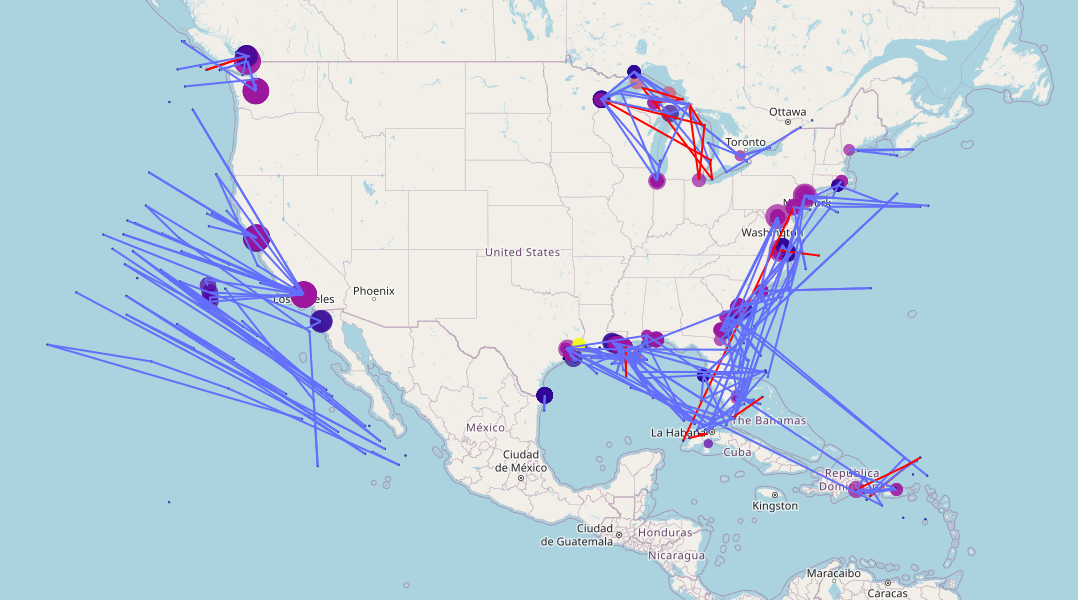
\includegraphics[width=0.5\textwidth]{map_cluster_1.png}
		\end{figure}
		
		Originalmente, se estimó implementar una versión para el algoritmo k-Means vectorial (\cite{ferreira2012vectorfieldkmeansclustering}). En la imagen \ref{map_cluster_1} se muestra la captura de señales AIS de cada barco cada veinticuatro horas durante un periodo de catorce días en septiembre de 2024. Sin embargo, dadas las complejidades inherentes al algoritmo se decidió probar otras vías.
		
		%Incluir pie de página para: 1 = at anchor, 5 = moored
		De una manera mucho más simple, se decidió reciclar los datos obtenidos entonces, para esta vez filtrar qué barcos se encontraban atracados o con el motor parado y cerca de las costas. Según la documentación aportada por el NOAA (agencia federal atmosférica de Estados Unidos), la tabla de datos incluía una variable 'Status' entre los cuales los valores '1' y '5' correspondían con esos casos (\cite{NOAA_AIS_DataDictionary} y \cite{MarineTraffic_AIS_Status}). En la imagen \ref{map_cluster_2} se muestra un mapa con aquellos barcos con dichos status.
		
		\begin{figure}[H]
			\caption{\label{map_cluster_2} Señales AIS de barcos atracados o con movilidad restringida recopilados por el NOAA}
			\centering
			\hspace*{1cm}
			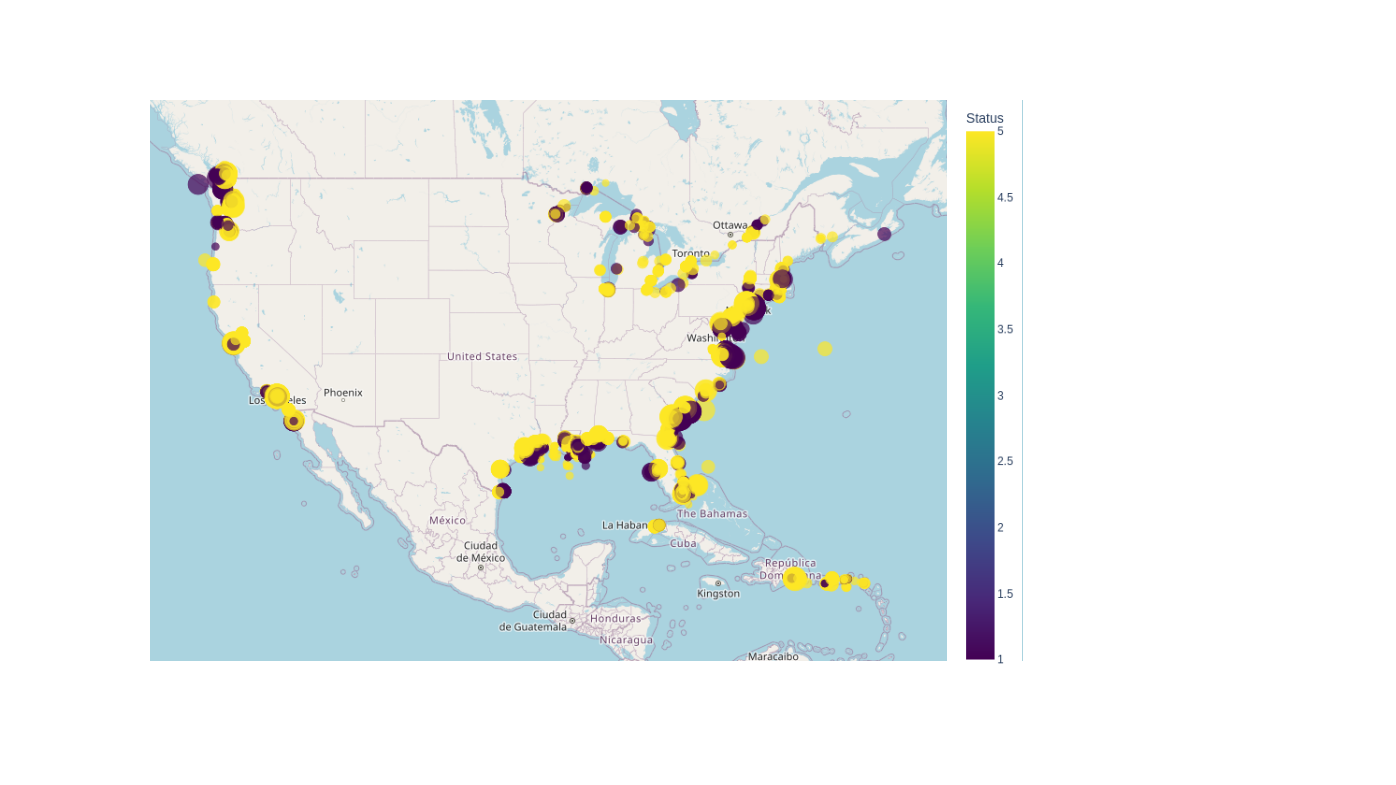
\includegraphics[width=0.8\textwidth]{map_cluster_2.png}
		\end{figure}
	
		Una vez filtrados los barcos con ese status (y con proximidad al litoral), se pudo realizar la agrupación basándose exclusivamente en las variables de coordenadas (latitud y longitud). Se implementó un problema de clustering haciendo uso del algoritmo k-Means con la métrica de 'silhouette' como método de evaluador de la calidad, para agrupar los barcos próximos a la costa en una treintena clusters. De entre estos clusters, finalmente se obtuvieron los potenciales hubs portuarios para considerar dentro del análisis (Véase la imagen \ref{map_cluster_3}).
		
		\begin{figure}[H]
			\caption{\label{map_cluster_3} Señales AIS de barcos atracados o con movilidad restringida recopilados por el NOAA}
			\centering
			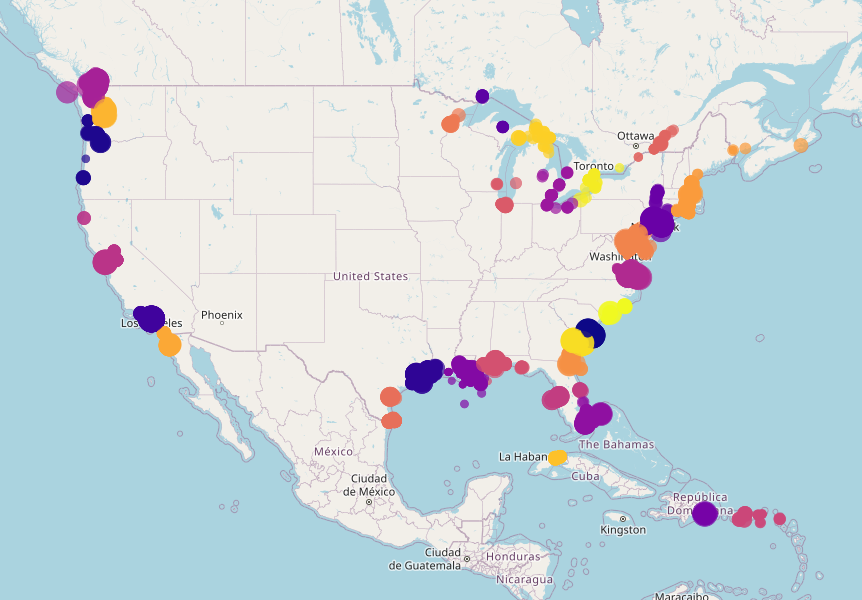
\includegraphics[width=0.5\textwidth]{map_cluster_3.png}
		\end{figure}
		
		 El resultado fue la asignación de coordenadas esféricas a cada centroide del cluster. Todo ello a partir de las señales emitidas por los barcos mercantes y detectadas por la agencia meteorológica de EE UU durante quince días del mes de septiembre de 2024. Estas coordenadas sirvieron para estimar de forma aproximada barcos atracados en puertos próximos entre sí y, en último término, asignarlas a oficinas del CBP. Gracias al conocimiento geográfico de Estados Unidos, no fue demasiado complicado asignar los hubs portuarios a las agencias aduaneras.
		 
		 Debido a las complejidades y adversidades del problema, finalmente se decidió incluir hasta seis hubs portuarios: (Newark (\cite{panynj2025facts}), Miami/Fort Lauderdale (\cite{porteverglades2025stats}), Houston (\cite{porthouston2025teus}), SFBA, Seattle/Tacoma (\cite{nwseaportalliance2025cargo}) y Área Metropolitana del Gran Los Ángeles (\cite{portla2025containerstats})) para el objeto de estudio.
		 
		 \underline{Pivote de las variables sobre incautaciones de drogas}\\
		 Por su parte, los datos provenientes de los datasets sobre incautaciones por parte de los "Field Office" (u oficinas de campo/regionales, \cite{cbp2025drugseizures}) tuvieron que pasar de una estructura "table longer" a una "table wider" para así poder encajar mes a mes con los datos de estibado de contenedores (\cite{cbp2022drugseizures}). Además, pivotando respecto al tipo de drogas, se logró generar todas las variables de conteo de redadas y de cantidad incautada para cada tipo de droga. Generando así un dataset más rico en término de variables.
		 
		 Una muestra de los datos originales publicados por el CBP para el caso de Nueva York:
		\begin{figure}[H]
			\caption{\label{cbp_ny_ori} Datos brutos del CBP para NY}
			\centering
			\hspace*{1cm}
			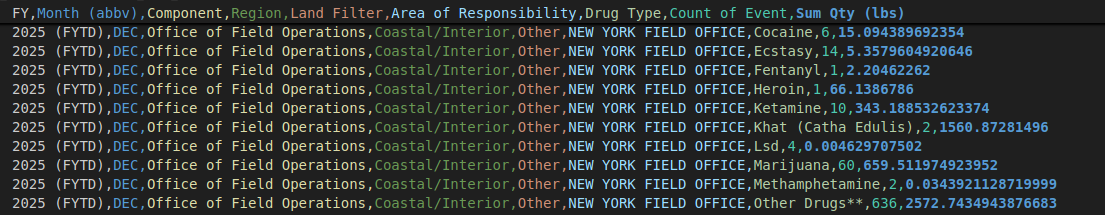
\includegraphics[width=\textwidth]{cbp_ny_ori.png}
		\end{figure}
	
		La captura de la figura \ref{cbp_ny_ori} es un fragmento del fichero csv correspondiente a los datos para los años fiscales 2022 a 2025 a nivel nacional disponible en la web del CBP (\cite{cbp2025drugseizures}).
		
		Con los datos de la figura \ref{cbp_ny_ori} hubo que hacer un análisis variable a variable para entender qué significaba y cuáles podrían ser incluidas en el dataset original.
		
		\begingroup
		\begin{table}[H]
			\centering
			\caption{\label{original_CBP}Descripción de las variables del conjunto de datos original del CBP}
			\label{tabla_variables}
			\begin{tabular}{|l|l|p{7cm}|p{4cm}|}
				\hline
				\textbf{Data} & \textbf{Variable} & \textbf{Description} & \textbf{Examples} \\
				\hline
				FY & Fiscal Year & Año fiscal en el que tuvo lugar el incidente & 2018, 2019, 2020, 2021 (FYTD) \\
				\hline
				Month (abbv) & Month & Mes (abreviado) en el que tuvo lugar el incidente & JAN, FEB, MAR \\
				\hline
				Component & CBP Component & Quién en el CBP estuvo liderando las incautaciones & Office of Field Operations (OFO), U.S. Border Patrol (USBP), Air and Marine Operations (AMO) \\
				\hline
				Region & Border Region & Región fronteriza en la ocurrió el incidente; las regiones fronterizas estñan definidas por cada componente & Coastal/Interior, Northern Border, Southern Border \\
				\hline
				Land Filter & Border Type & La parte de la región fronteriza rodeada por mar o tierra & Land Only, Other \\
				\hline
				Area of Responsibility or Branch & Field Office/Sector/Branch & La oficina de campo, sector o rama en la que ocurrió el incidente & Atlanta Field Office, Big Bend Sector, Laredo Air Branch \\
				\hline
				Drug Type & Seized Drug Type & La categoría de droga en la que se produjo el incidente & Cocaine, Fentanyl, Heroin, Marijuana \\
				\hline
				Count of Event & Seizure Count & Número de redadas/incautaciones por tipo de droga & Discrete variable \\
				\hline
				Sum Qty (lbs) & Seized Quantity & Cantidad de droga incautada en libras (lbs) & Continuous variable \\
				\hline
			\end{tabular}
		\end{table}
		\endgroup
		
		A los datos tratados del CBP para los años fiscales 2022 a 2025 se les unieron todos los años disponibles en la página web oficial (hasta el año 2019).
		
		Para el modelo interesaba:
		\begin{itemize}
			\item [-] Unificar las variables 'FY' y 'Month (abbv)' en una variable denominada 'Date' con formato 'YYYY-MM'
			\item [-] Asignar a cada 'Area of Responsibility' las coordenadas de su hub portuario asociado
			\item [-] Seleccionar las variables 'Drug Type', 'Count of Event' y 'Sum Qty (lbs)'
		\end{itemize}
	
		Un pequeño fragmento de código con dichas transformaciones (para el caso particular de Newark/Nueva York) se muestra en las siguientes líneas (en la sección de Anexos se pone a disposición una versión más completa)
		
		\begin{verbatim}
			# drug_seizures combined es un dataframe compuesto por
			# todos los ficheros recopilados desde el año fiscal 2019 hasta 2025
			drug_seizures_combined = drug_seizures_combined.loc[drug_seizures_combined
			['Area of Responsibility'] == 'NEW YORK FIELD OFFICE']
			
			drug_seizures_combined['Date'] = drug_seizures_combined['FY'] + '-' +
			 drug_seizures_combined['Month (abbv)'].astype(str)
			 
			# Convert 'Date' column to datetime format and then to '%Y-%m'
			drug_seizures_combined['Date'] = pd.to_datetime(drug_seizures_combined['Date'],
			format='%Y-%b').dt.strftime('%Y-%m')
			
			# Drop the original 'FY' and 'Month (abbv)' columns if no longer needed
			drug_seizures_combined.drop(columns=['FY', 'Month (abbv)', 'Component', 'Region', 
			'Land Filter', 'Area of Responsibility'], inplace=True)
		\end{verbatim}
	
		
		Una vez seleccionadas y modificadas estas columnas, como se ve en la sección de código justo anterior, se produjo un drop de la variable 'Area of Responsibility' y para ello, se generaron dos nuevas ('latitude' y 'longitude') que la sustituyesen e hiciesen de identificadores, en este caso, para la región de Nueva York/Nueva Jersey:
		
		\begin{verbatim}
			# row 6: NJ/NY, El id=6 corresponde al hub portuario de Newark (ver Anexos)
			drug_seizures_combined['latitude'] = us_port_hubs.loc[6, 'coord_0']
			drug_seizures_combined['longitude'] = us_port_hubs.loc[6, 'coord_1']
		\end{verbatim}
	
		Por último, en cuanto a la manipulación del subconjunto de datos correspondiente a las incautaciones de drogas, se realizó un pivote de las variables correspondientes. Con el fin de tener un conjunto de variables que pudieran acoplarse más adelante a los datos de actividad portuaria se realizó la siguiente acción 'pivot\_table' definida en pandas:
		
		\begin{verbatim}
			drug_seizures_wide=pd.pivot_table(drug_seizures_combined,index=['Date','latitude','longitude'],
			columns='Drug Type', values=['Count of Event', 'Sum Qty (lbs)'], aggfunc='sum')...
		\end{verbatim}
	
		Tras esta transformación, las variables definidas originalmente tanto en \ref{original_CBP} como su muestra de datos en \ref{cbp_ny_ori} quedaron así (nota aquí solo se representa una pequeña porción de variables, todas las variables se encuentran disponibles en la sección de Anexos):
		
		\begin{itemize}
			\item Date
			\item Latitude
			\item Longitude
			\item Count of Event\_Cocaine
			\item Count of Event\_Marijuana
			\item Count of Event\_Other Drugs**
			\item Sum Qty (lbs)\_Cocaine
			\item Sum Qty (lbs)\_Marijuana
			\item Sum Qty (lbs)\_Other Drugs**
		\end{itemize}
		
		Con una pequeña muestra de incautaciones de cocaína y marihuana en Nueva York para cinco meses de 2024:
		
		\begingroup
		\small
		\begin{table}[H]
			\caption{Incautaciones de Cocaína y Marihuana en 2024 en NY}
			\label{tabla_incautaciones_2024}
			\begin{center}
			\begin{tabular}{|c|c|c|c|c|c|c|}
				\hline
				\textbf{Date} & \textbf{Latitude} & \textbf{Longitude} & \textbf{\#Coc$^a$} & \textbf{\#Marij$^b$} & \textbf{Qty Cocaine$^c$} & \textbf{Qty Marijuana$^d$} \\
				\hline
				2024-08 & 40.690946 & -74.157057 & 10.0 & 1128.0 & 39.545198 & 3512.319660 \\
				\hline
				2024-09 & 40.690946 & -74.157057 & 26.0 & 170.0 & 165.036418 & 899.509971 \\
				\hline
				2024-10 & 40.690946 & -74.157057 & 9.0 & 110.0 & 51.562375 & 1140.032954 \\
				\hline
				2024-11 & 40.690946 & -74.157057 & 6.0 & 118.0 & 27.847470 & 1375.535637 \\
				\hline
				2024-12 & 40.690946 & -74.157057 & 6.0 & 60.0 & 15.094390 & 659.511975 \\
				\hline
			\end{tabular}
			\end{center}
			$^a$ Count of Event Cocaine \\
			$^b$ Count of Event Marihuana \\
			$^c$ Sum Qty (lbs) Cocaine \\ 
			$^d$ Sum Qty (lbs) Marihuana
		\end{table}
		\endgroup
		

		\underline{Asignación de un hub portuario con una agencia aduanera}\\
		Tras la transposición de los datos de incautaciones de drogas proporcionados por los documentos del CBP (detallado anteriormente), junto con la generación de la variable 'Hub Portuario' (mediante el clustering también definido), se pudo vincular los datos de las incautaciones de la oficina de campo del CBP a su hub portuario más indicado.
		
		Sobre por qué se decidió asignar cada oficina del CBP al hub portuario, en las fuentes originales se menciona que en el caso de los datasets referidos a "Nationwide Drug Seizures: Los agentes y oficiales del CBP prohiben la entrada y salida de productos narcóticos ilícitos a través de sus fronteras y en los puertos de entrada" (\cite {cbp2025drugseizures}). Es decir, se hace referencia explícita sobre los datos se refieren, en parte, a incautaciones en puertos. Esto es útil para el planteamiento del problema frente a otras fuentes de datasets del mismo CBP que hacían referencia a AMO (Operaciones marinas y aéreas cuyo alcance o jurisdicción quedaba más laxa* \cite{cbp2025amodrugseizures}). Sin embargo, los retardos y acumulaciones en las incautaciones de los segundos, no hacen evidente la relación entre la actividad portuaria con la cantidad de droga detectada. Más adelante se dejará constancia de terceros factores que pudieran influir en el análisis.
		
		Tras todo lo comentado en el anterior párrafo, un caso que hubiese sido interesante de incluir en los datos hubiese sido el de una ciudad fronteriza como San Diego. Sin embargo, no se lograron encontrar datos de suficiente calidad que pudieran ser integrados y provistos por la autoridad portuaria del puerto de San Diego \cite{portofsandiego2025}.
		
		% Incluir código de integración de datos de drogas con puertos.
		A continuación se muestra un pequeño fragmento de código mostrando como se integraron los datos de incautaciones de drogas recopilados por el CBP de Nueva York, con los datos de actividad del puerto de Newark:
		
		\begin{verbatim}
			
			# Join de los datos del puerto de newark con 
			NJNY_data = pd.merge(teu_data_newark, drug_seizures_wide, on='Date', how='inner')
		\end{verbatim}
	
		(*) Se advierte al lector que se han estado mostrando exclusivamente ejemplos de código para el puerto de Newark/Nueva York. El mismo proceso paso a paso fue seguido para el resto de puertos analizados.
		
		\underline{Generación de la variable 'Sum of Counts'}\\
		Tras haber realizado el pivote de los datos de incautaciones de drogas para poder saber la cantidad y el número de drogas por cada tipo de droga y para cada mes, se generó una variable "Sum of Counts", la cual será desarrollada en la subsección \ref{feature engineering}. La motivación en este caso, se fundamentó en la necesidad de agrupar un dato global y la inviabilidad de hacerlo sumando las cantidades (sea en kilogramos o libras) para tipos de drogas tan diferentes entre sí, junto con otros aspectos: el valor estimado, el nivel de adicción, letalidad...
		 
		\underline{El dataset construido en este proceso}\\
		Tras haber estudiado las fuentes originales, haber operado de modo que se pudieran compatibilizar los dos distintos ámbitos de estudio (el análisis del tráfico marítimo con la incautación de drogas) y la integración de los mismos en sentido último, se fueron generando, en primer lugar, un conjuntos de datos para cada hub portuario y finalmente un conjunto de datos que integraba los distintos hubs portuarios en un mismo dataset.\cite{} 
		
		% Dibujo con la estructura del dataframe a nivel general
		
		A nivel técnico, como se mencionó unas líneas más arriba, esta integración entre distintas fuentes (actividad portuaria con incautaciones de droga) se realizó mediante operaciones "merge" proporcionadas por la librería de pandas.
		
		El resultado es un conjunto de datos con las siguientes variables:
		
		\begin{itemize}
			\item Loaded Imports
			\item Empty Imports
			\item Loaded Exports
			\item Empty Exports
			\item Total TEUs
			\item Date
			\item Total Imports
			\item Total Exports
			\item Latitude
			\item Longitude
			\item Count of Event\_Cocaine
			\item Count of Event\_Ecstasy
			\item Count of Event\_Fentanyl
			\item Count of Event\_Heroin
			\item Count of Event\_Ketamine
			\item Count of Event\_Khat (Catha Edulis)
			\item Count of Event\_LSD
			\item Count of Event\_Marijuana
			\item Count of Event\_Methamphetamine
			\item Count of Event\_Other Drugs**
			\item Sum Qty (lbs)\_Cocaine
			\item Sum Qty (lbs)\_Ecstasy
			\item Sum Qty (lbs)\_Fentanyl
			\item Sum Qty (lbs)\_Heroin
			\item Sum Qty (lbs)\_Ketamine
			\item Sum Qty (lbs)\_Khat (Catha Edulis)
			\item Sum Qty (lbs)\_LSD
			\item Sum Qty (lbs)\_Marijuana
			\item Sum Qty (lbs)\_Methamphetamine
			\item Sum Qty (lbs)\_Other Drugs**
			\item \textcolor{red}{Sum\_of\_Counts}
		\end{itemize}
	
		Dado que se trata de un problema en el que se busca hallar la actividad del narcotráfico (sea como se defina ésta) con la actividad portuaria (estiba de contenedores), está claro que conjunto de variables son potenciales predictoras y cuáles son potenciales objetivo.
		
		Para el primer caso es sencillo: todas las relacionadas con operaciones sobre contenedores: 
		\begin{itemize}
			\item Loaded Imports
			\item Empty Imports
			\item Loaded Exports
			\item Empty Exports
			\item Total TEUs
			\item Date
			\item Total Imports
			\item Total Exports
		\end{itemize}
	
		Y entre las restantes, tocará más adelante analizar su comportamiento con los predictores e, incluso, generar nuevas variables (en color rojo una de estas variables que será definida más adelante).
		
		\underline{Fort-Lauderdale tuvo un comportamiento particular}\\
		Un caso particular en la integración de datos se correspondió con los extraídos del Puerto de Everglades en Fort-Lauderdale (Área Metropolitana de Miami, Florida). Se reseña que no se pudieron incluir los datos del puerto de Miami por falta de calidad de los mismos (falta de granularidad, acuerdos de proceso de contenedores con operadores privados en los terminales que podían dificultar la integración de los datos \cite{portmiami2025cargo}, etc.). Los datos fueron extraídos de los informes para cada año fiscal a disposición en \cite{porteverglades2025stats}. En algún caso particular, se observó la ausencia de datos para el año fiscal 2021 (últimos tres meses, \cite{porteverglades2021teus}). El tratamiento de estos missing values será desarrollado en su sección correspondiente \ref{preprocessing}.
		
		\subsubsection{\label{feature engineering}Ingeniería de características}
		Antes de realizar las primeras visualizaciones ya se vislumbraron determinadas certezas respecto a los datos brutos que componían el dataset primitivo y, de paso, se estimó necesario la inclusión de otras variables que fuesen generadas a partir de éstas primeras.
		% Generación del target (y posibles alternativas)
		Esto se debe a que en ningún caso de los datos originales, se veía con claridad que alguna variable pudiera ser considerada objetivo de las variables de contenedores. Excepto, como se muestra en la lista de variables del dataset construido en \ref{data origin}, la variable "sum of counts". 
		
		Esta subsección va a servir como propósito para no solo mostrar la generación de ciertas variables a partir de las variables originales (proceso de feature engineering), sino también para incluir nuevas ideas que pudieran ser aportadas para otros trabajos que siguiesen en la misma línea.
		
		\underline{Sum of Counts}\\
		Uno de los puntos que más quebraderos de cabeza trajo respecto al desarrollo del trabajo fue, por encima de todo, qué variable se usaría como target para el modelo. Pese a que este punto será abordado con mayor profundidad en la sección \ref{implementacionPractica}, pronto surgió la idea de incluir una variable que agrupase todas las incautaciones (número de redadas) sin importar la categoría de la droga para un mismo mes y una misma región. Esto no era posible de realizar sobre la cantidad de droga incautada (masa en libras) ya que carecía de sentido mezclar masas de distintos orígenes. También se llegó a pensar en hacer la suma del valor incautado, pero también se descartó por la falta de datos al respecto y, que la influencia del mismo valor al igual que la masa generase ciertas distorsiones entre una región u otra.
		
		La variable "sum of counts" se define, entonces, como la suma de redadas mensuales para cada tipo de droga. A continuación se formula su expresión matemática:
		
		% Sumatorio por count event de tipo de drogas:
		$$
		Sum\; of\; Counts = \sum_i C_{count\; event,i}
		$$
		%
		Donde $i$ es cada tipo de droga.
		
		Como observación, la generación de esta variable se realizó sobre los datos brutos antes de su estandarización, aunque en la práctica el efecto hubiese sido el mismo. En la siguiente tabla se muestra el número de redadas promedio por mes para cada puerto.
		
		%Tabla con incautaciones por droga + sum of counts
		\begingroup
		\small
		\begin{table}[H]
			\begin{center}
				\caption{Incautaciones de drogas por puerto}
				\label{tabla_incautaciones}
				\setlength{\tabcolsep}{1pt}
				\begin{tabular}{|l|c|c|c|c|c|c|c|c|c|c|c|}
					\hline
					\textbf{Puerto} & \textbf{Cocaína} & \textbf{Éxtasis} & \textbf{Fen$^a$} & \textbf{Her$^b$} & \textbf{Ket$^c$} & \textbf{Khat} & \textbf{LSD} & \textbf{Mari$^d$} & \textbf{Meth$^e$} & \textbf{Otras} & \textbf{Total} \\
					\hline
					Houston & 2.98 & 4.29 & 3.00 & 1.38 & 4.72 & 1.89 & 2.16 & 68.47 & 3.26 & 55.27 & 134.19 \\
					Los Ángeles$^*$ & 10.07 & 14.69 & 1.86 & 2.17 & 11.67 & 2.31 & 6.19 & 160.93 & 24.24 & 279.15 & 504.99 \\
					Fort Lauderdale & 49.24 & 21.21 & 5.38 & 1.70 & 16.85 & 2.94 & 19.53 & 115.00 & 5.39 & 1008.00 & 1237.28 \\
					Newark & 43.92 & 297.08 & 5.52 & 93.37 & 46.60 & 8.59 & 176.66 & 129.27 & 53.97 & 1557.47 & 2398.60 \\
					Oakland & 9.27 & 19.62 & 9.35 & 1.60 & 3.83 & 5.17 & 10.45 & 87.47 & 32.61 & 120.32 & 276.40 \\
					Seattle/Tacoma & 5.93 & 4.98 & 2.11 & 1.83 & 2.65 & 1.86 & 9.47 & 146.16 & 4.22 & 60.33 & 227.20 \\
					\hline
				\end{tabular}
			\end{center}
			$^a$ Fentanilo \\
			$^b$ Heroína \\
			$^c$ Ketamina \\ 
			$^d$ Marihuana \\
			$^e$ Metanfetamina \\
			$^*$ Los datos incluyen tanto el puerto de Los Ángeles como de Long Beach.
		\end{table}
		\endgroup
		
		\underline{Ratios por Tipo de Droga}\\
		Una vez generada la variable "Sum of Counts", era posible tener una asignación de cada puerto con la cantidad total de redadas mensuales. Pero para cada una de esas redadas se consideró que aportaría valor el conocer cómo eran: si lograban continuamente capturar gran cantidad de estupefacientes, si en cambio, solían ser pequeñas incautaciones con algún "premio" en forma de gran redada... Si esto dependía del tipo de droga y/o del hub portuario. Para ello se fueron creando las variables "Ratio\_" para cada tipo de droga. Su cálculo no es más que el cociente entre la cantidad incautada de un tipo de droga durante un mes en una región y el número de redadas durante ese mes en esa misma región.
		
		A continuación se muestran una serie de gráficas que muestran la relación entre la cantidad de droga incautada con el número de redadas. Nótese que las figuras representadas son anteriores al análisis y exclusión de outliers:
		
		\begin{figure}[H]
			\caption{\label{graph_ratios_1} Relación entre la cantidad de cocaína incautada y el número de redadas por puerto}
			\centering
			\hspace*{1cm}
			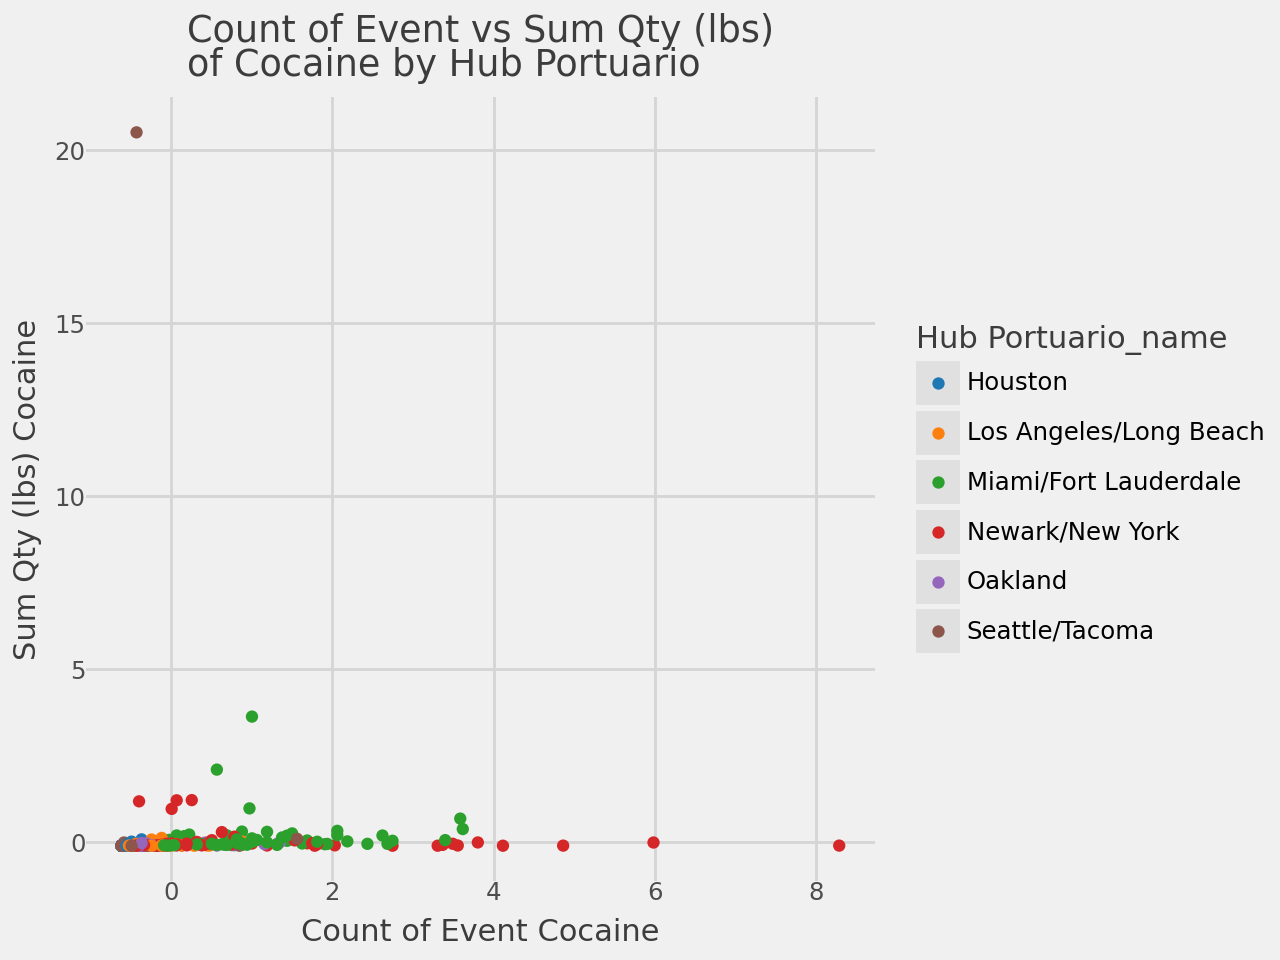
\includegraphics[width=0.8\textwidth]{graph_ratios_1.png}
		\end{figure}
		
		Como se puede figurar, la variable ratio sirve para identificar redadas comunes frente operaciones sobresalientes en las que en una redada se incauta una gran cantidad de un tipo de droga. Dado que la cantidad de droga (o su volumen) varía de un tipo a otra, habrá tipos de redadas que tengan un valor del ratio mayor que en las demás. Obsérvense los casos para los datos de cocaína (figura \ref{graph_ratios_1}) con una presunta redada en Seattle/Tacoma con una gran cantidad de libras incautadas. O las distintas redadas de heroína en Nueva York, próxima al puerto de Newark (figura \ref{graph_ratios_2}).
		
		\begin{figure}[H]
			\caption{\label{graph_ratios_2} Relación entre la cantidad de heroína incautada y el número de redadas por puerto}
			\centering
			\hspace*{1cm}
			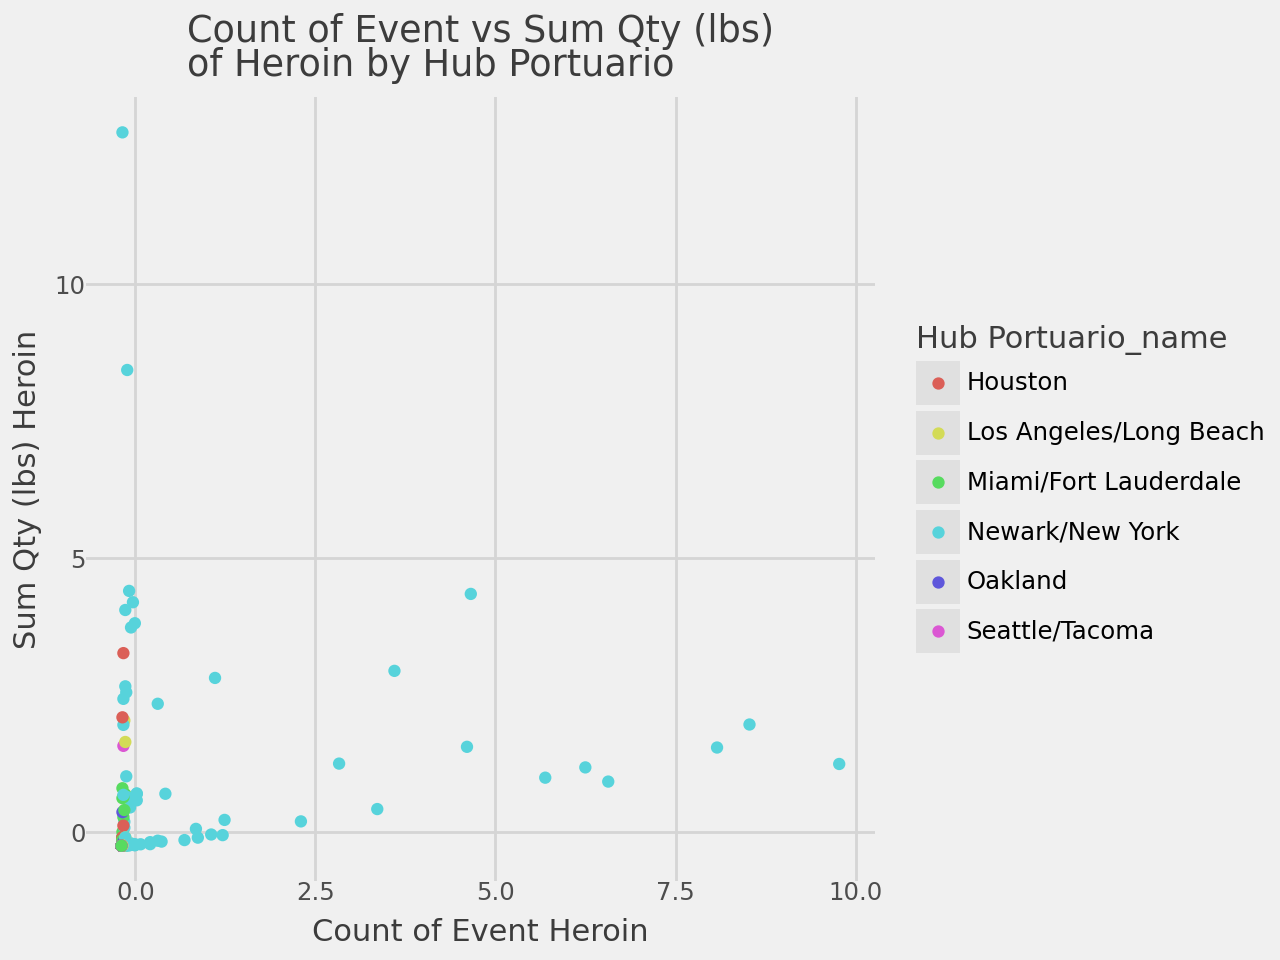
\includegraphics[width=0.75\textwidth]{graph_ratios_2.png}
		\end{figure}
		
		\begin{figure}[H]
			\caption{\label{graph_ratios_3} Relación entre la cantidad de marihuana incautada y el número de redadas por puerto}
			\centering
			\hspace*{1cm}
			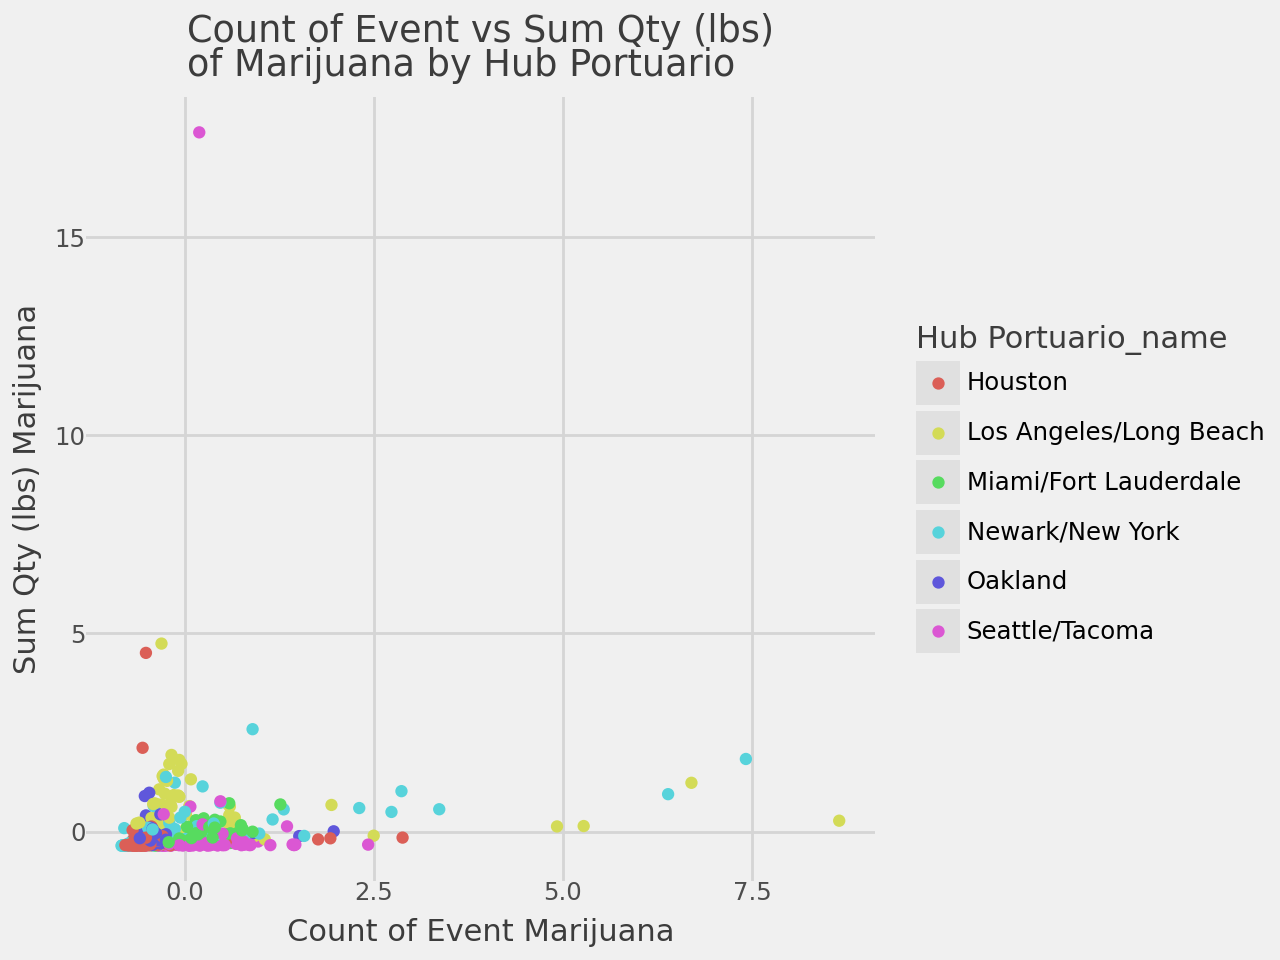
\includegraphics[width=0.75\textwidth]{graph_ratios_3.png}
		\end{figure}
		
		En la figura inmediatamente superior (figura \ref{graph_ratios_3}), se observan los datos que servirán para generar la variable "ratio marihuana". A destacar una redada importante en Seattle. Los puertos de Los Angeles y Newark suelen tener de media más incautaciones en este caso. Aunque se recuerda al lector que pese a que la marihuana está legalizada en algunos estados como California, en este trabajo se trata con los datos registrados como tal.
		
		\begin{figure}[H]
			\caption{\label{graph_ratios_4} Relación entre la cantidad de otras drogas incautadas y el número de redadas por puerto}
			\centering
			\hspace*{1cm}
			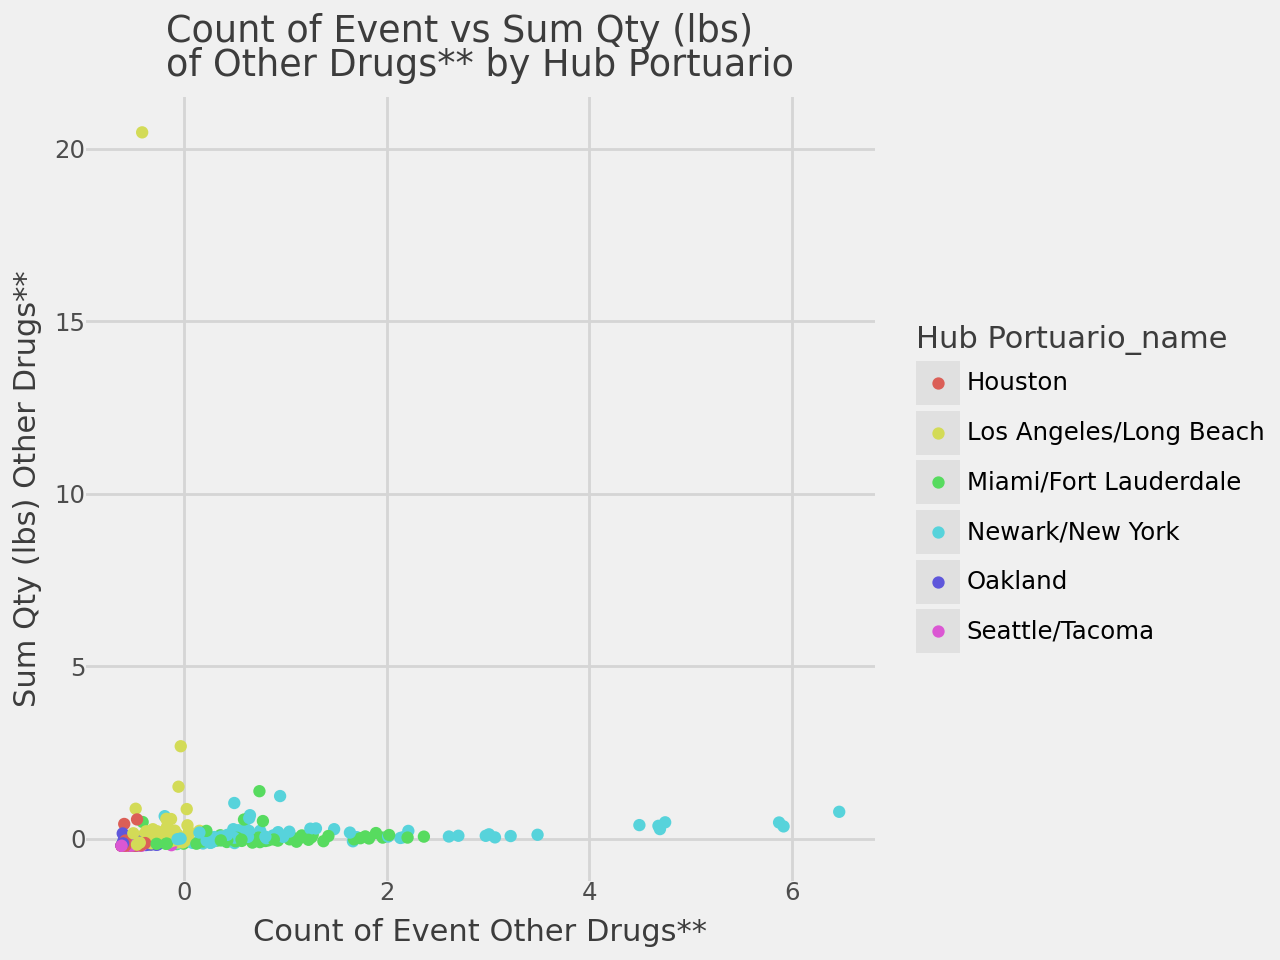
\includegraphics[width=0.75\textwidth]{graph_ratios_4.png}
		\end{figure}
		
		Tras estas visualizaciones gráficas entre la cantidad de droga incautada y el número de redadas exitosas respecto a esa misma droga, ahora toca dar forma y finalidad a la variable que se quiere generar a partir de ellas.
		
		Si bien es cierto que en las representaciones no se han omitido los outliers, se trata como bien se dice, de meras representaciones gráficas. Aquí la nueva variable es el cociente entre las dos variables anteriores. A continuación se muestra su expresión matemática: 
		% Incluir cálculo "Ratio_"
		% Cociente entre count event de tipo de drogas:
		$$
		Ratio\; of\; Drug\; Type = \frac{Sum\; Qty_i}{Count\; of\; Event_i}
		$$
		%
		Donde $i$ es cada tipo de droga.
		
		%Visualización en un mapa de Max Ratios:
		Tras generar esta variable, toca comprobar como se comporta respecto al resto de variables del conjunto de datos. En la subsección \ref{preprocessing} ya se mostraron alguas representaciones gráficas sobre el comportamiento de las variables "ratio" (ver las figuras \ref{st_ratio_3} o \ref{outliers_2}) mucho antes de que fuesen definidas.
		
		Por otro lado, a continuación se muestran algunas visualizaciones para cada variable del tipo "Ratio" para cada tipo de droga en cada puerto:
		
		\begin{figure}[H]
			\caption{\label{map_bubble_5} Principales redadas por tipo de droga en cada puerto}
			\centering
			\hspace*{1cm}
			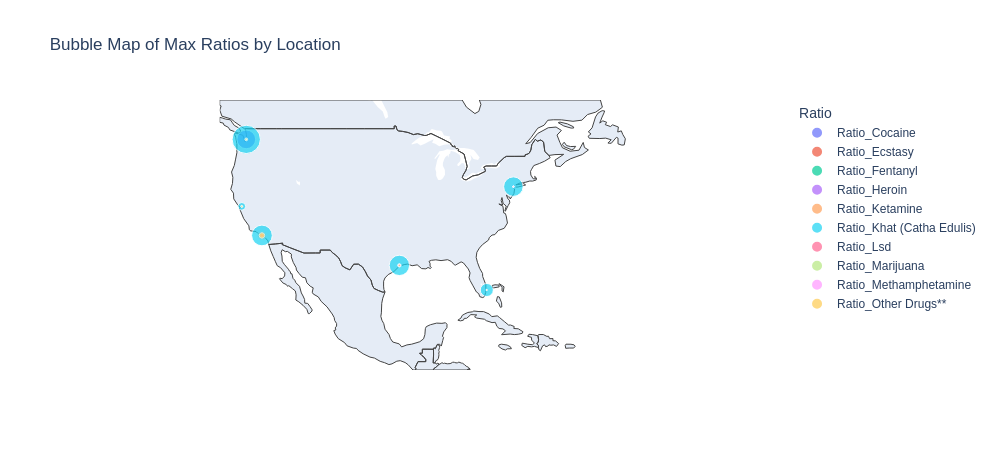
\includegraphics[width=\textwidth]{map_bubble_5.png}
		\end{figure}
		
		En todos los puertos se muestra que las redadas con mayor cantidad de droga incautada pertenecen a "Khat" debido a su poca implantación o dificultad para dar con ella. Véase la figura \ref{map_bubble_5}. Sin embargo, este tipo de drogas con pocos datos sobre ellas genera una cierta niebla e impresión distorsionada sobre grandes redadas. Para ver realmente el gran trabajo constante de incautación es mejor ver la figura \ref{map_bubble_6} en la que se muestra que entre los casos con más registros habituales (cocaína, heroína y otras drogas) donde se producen las principales incautaciones y cuanto representan respecto del total.
		
		\begin{figure}[H]
			\caption{\label{map_bubble_6} Principales redadas de otras drogas y demas en cada puerto}
			\centering
			\hspace*{1cm}
			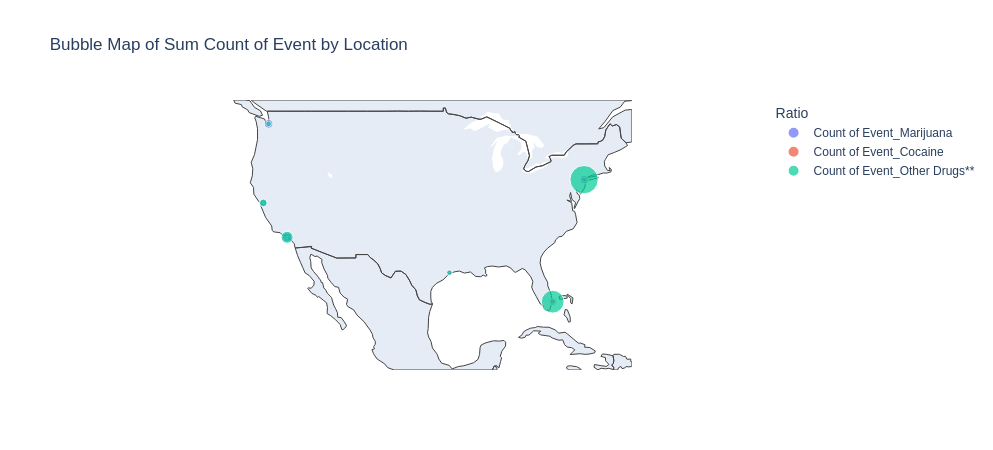
\includegraphics[width=\textwidth]{map_bubble_6.png}
		\end{figure}
		
		Como se mencionó en uno de los párrafos anteriores, con estas nuevas variables se buscaba ver a primera vista qué tipo de incautaciones se llevaban de forma regular para cada hub portuario. Por ejemplo, para los casos de incautaciones de cocaína, los puertos de Newark y de Miami eran constantes las redadas con importantes cantidades incautadas. Por otro lado, en Seattle/Tacoma se encontraron picos de incautación (similar a una delta) en algún mes concreto (Ver figura \ref{st_ratio_1} en la subsección \ref{preprocessing}).
		
		% Añadir alguna otra figura con ratio.
		Para el cálculo de las variables de ratio, se barajó realizar el cálculo a partir de los datos normalizados. Sin embargo, a la vista de resultados contradictorios, se decidió finalmente realizarlo sobre los datos brutos. Una de las contraindicaciones que surgía de esta última forma de calcularlo era la aparición de indeterminaciones del tipo $ \frac{0}{0}$ fruto de observaciones con missing values. Dado que los missing values correspondían a meses estimados sin redadas y, por lo tanto, sin incautaciones, y que el resto de valores eran forzosamente enteros positivos, el valor del ratio debía ser definitivamente, entero positivo, estrictamente mayor que cero. Estas aseveraciones permitieron, sin lugar a dudas, imputar los ratios en los casos de missing values a cero. Su sentido dentro del contexto de los datos de esa variable es que el cero es el mínimo valor para esa variable y que ninguna redada realizada podía alcanzar ese mínimo. Por su parte, el descarte de realizar el cálculo a partir de los datos normalizados era la paradoja resultante de obtener un ratio negativo (por debajo de la media) en el caso de tener una cantidad incautada elevada (valor positivo por encima de la media, numerador del cociente) frente un número bajo de redadas (valor negativo por debajo de la media, denominador del cociente) que, en relación con el resto de ratios, debería estar en el extremo positivo de la distribución. Finalmente, al igual que el resto de variables, antes de ser integradas en el dataset fueron estandarizadas mediante StandardScaler() implementado en el Pipeline de scikit-learn.
		
		% Pequeño esquema sobre proceso de generacion ratio sobre datos brutos + estandarización posterior.
		
		% Suavizados de señales originales.
		% Derivadas sobre suavizados.
		\underline{Otras feature engineering}\\
		Por otro lado, también se estimó realizar un modelo basado en la comparación de tendencias entre variables de entrada (relacionadas con la gestión de los contenedores) y si el volumen de carga en un puerto mantiene alguna relación con la variación en la cantidad de droga total incautada. En este caso, fueron otras prioridades y ciertas restricciones de tiempo las que dejaron de lado este acercamiento al problema que hubiese sido, sin duda alguna, muy interesante de plantear. En todo caso, para lograr intuir la tendencia de señales temporales con mucho ruido habría que haber aplicado un filtro que suavizase la señal original y después derivar.
		
		\underline{¿Por qué no se suman las cantidades de droga incautada?}\\
		Como se ha comentado con anterioridad en esta misma sección, pese a que hay elementos interesantes en favor de ello: la cantidad en kilogramos incautada de un tipo de droga A frente a otro tipo B no sería determinante a la hora de realizar un análisis y que podría inducir a error, quizá si lo fuese su equivalente en valor monetario -pero inviable en términos prácticos-.
		
		\subsubsection{\label{EDA}Análisis Exploratorio de los Datos}
		Una vez conformado el dataset, se realizó un primer análisis exploratorio de datos. Por un lado, se realizó uno para cada hub portuario gracias al manejo de herramientas y librerías de visualización de python como plotnine (\cite{plotnine2025}) o ydata-profiling (\cite{ydata2025profiling}). Por otro lado, también se estimó la importancia que pudieran tener las variables geográficas. En este último caso, se generaron mapas geográficos con la librería plotly (\cite{plotly2025python}).

		\underline{Análisis temporal (series temporales)}\\
		Dado que los datos reportados tienen un orden cronológico, se consideró la inclusión de un análisis de series temporales. Ciertas apariencias de los datos brutos daban lugar a estimar ese acercamiento. En las figuras \ref{timeseries_1} y \ref{timeseries_2} se observa el comportamiento en el puerto de Miami. Nótese que para la primera imagen los datos están estandarizados (ésta compara el número total de redadas en comparación con el trasiego de contenedores). Por su parte la segunda imagen desagrega "Sum of Counts" (Véase \ref{feature engineering}) en los distintos tipos de drogas. En este último caso, los datos aportados están en valores absolutos.
		\begin{figure}[H]
			\caption{\label{timeseries_1} Actividad (movimiento de cargamento) en el puerto de Fort Lauderdale}
			\centering
			\hspace*{1cm}
			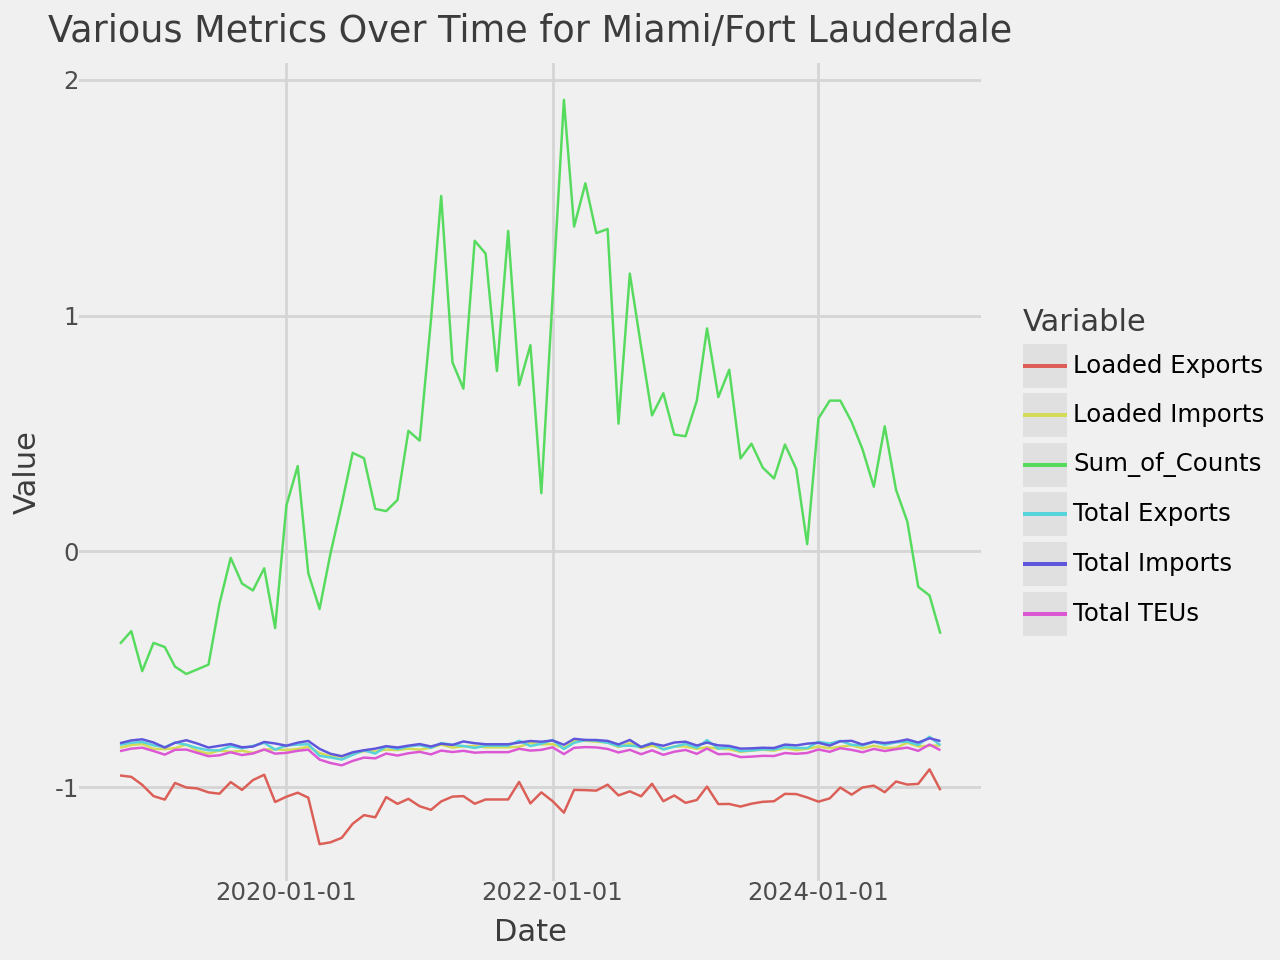
\includegraphics[width=0.8\textwidth]{timeseries_1.png}
		\end{figure}
	
		\begin{figure}[H]
			\caption{\label{timeseries_2} Redadas en el puerto de Fort Lauderdale}
			\centering
			\hspace*{1cm}
			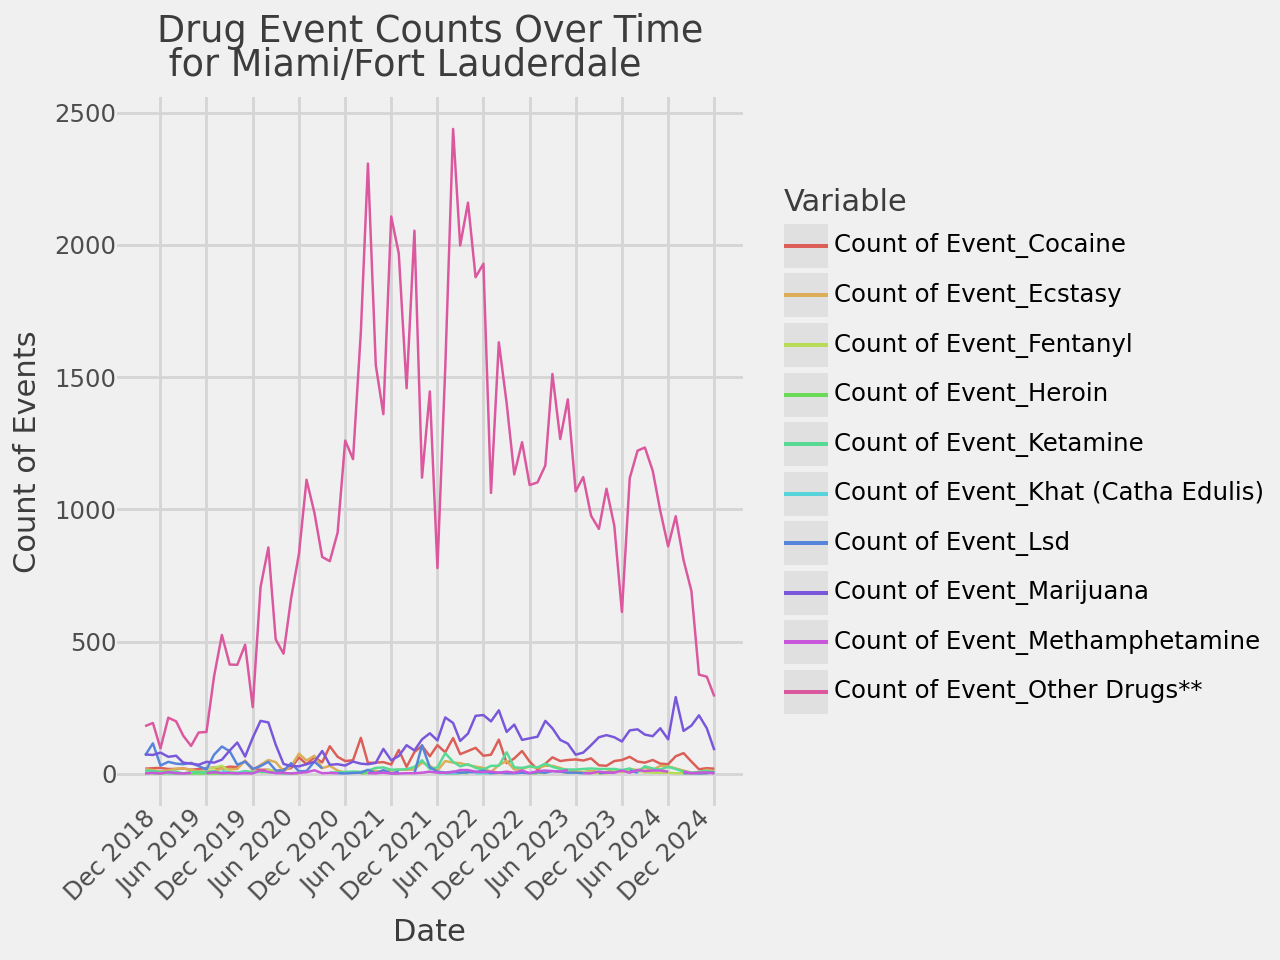
\includegraphics[width=0.8\textwidth]{timeseries_2.png}
		\end{figure}
	
		Las conclusiones son evidentes respecto a la influencia que tiene "Other Drugs" dentro de las incautaciones en el puerto de Fort Lauderdale.
	
		\begin{figure}[H]
			\caption{\label{timeseries_6} Redadas incautando cocaína por puerto}
			\centering
			\hspace*{1cm}
			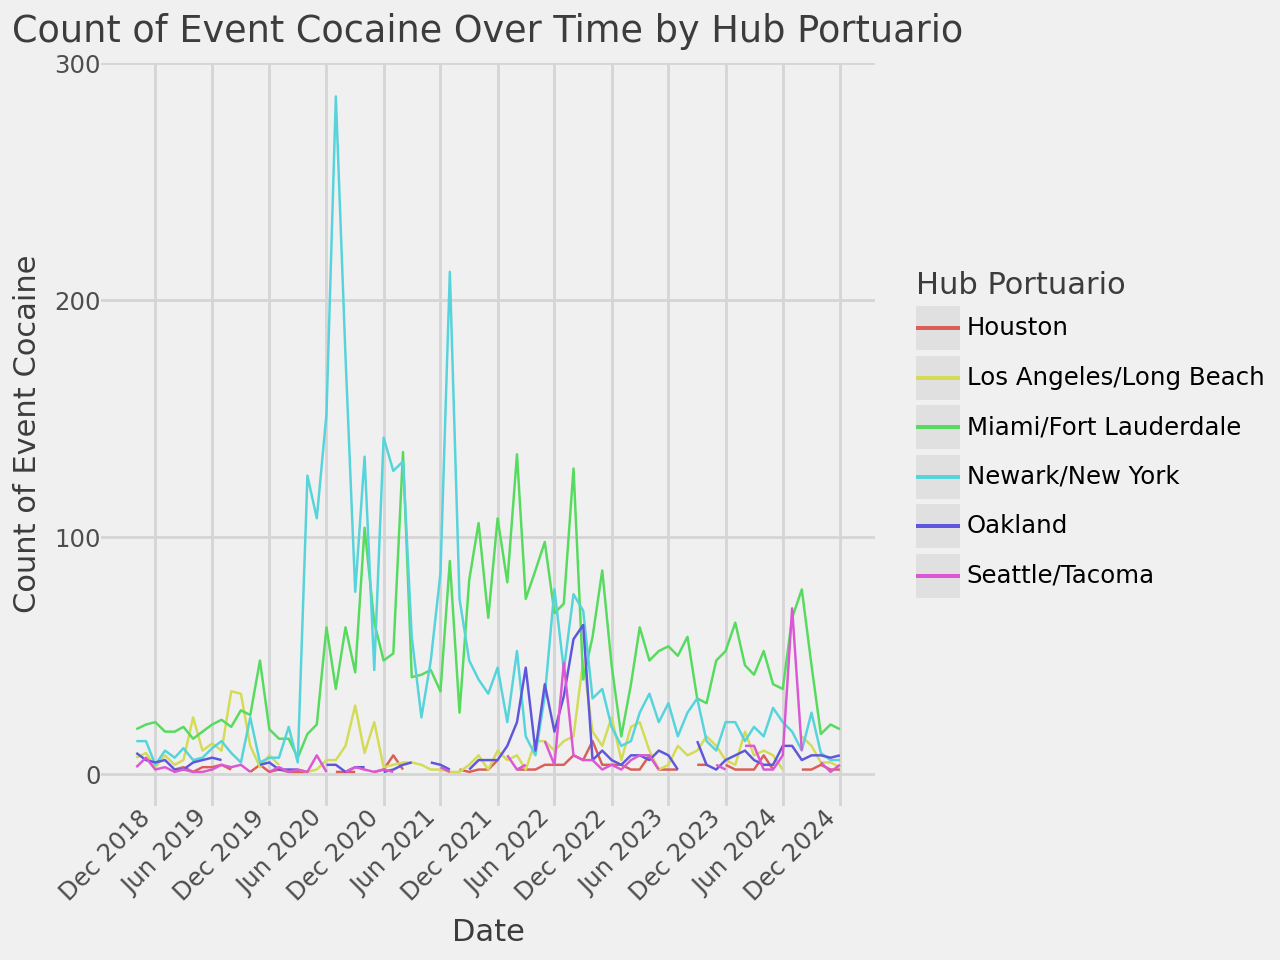
\includegraphics[width=0.8\textwidth]{timeseries_6.png}
		\end{figure}
	
		En la figura \ref{timeseries_6} se muestra la cantidad total de redadas de cocaína para cada hub portuario. Véase que los datos aportados están en valor absoluto (y se dejan las figuras \ref{timeseries_7} y  \ref{timeseries_8} para comparar visualmente la escala entre las redadas de cocaína con respecto a heroína y éxtasis). Como se observa, hay muchas menos redadas de la primera que de las dos últimas.
		
		\begin{figure}[H]
			\caption{\label{timeseries_7} Redadas incautando éxtasis por puerto}
			\centering
			\hspace*{1cm}
			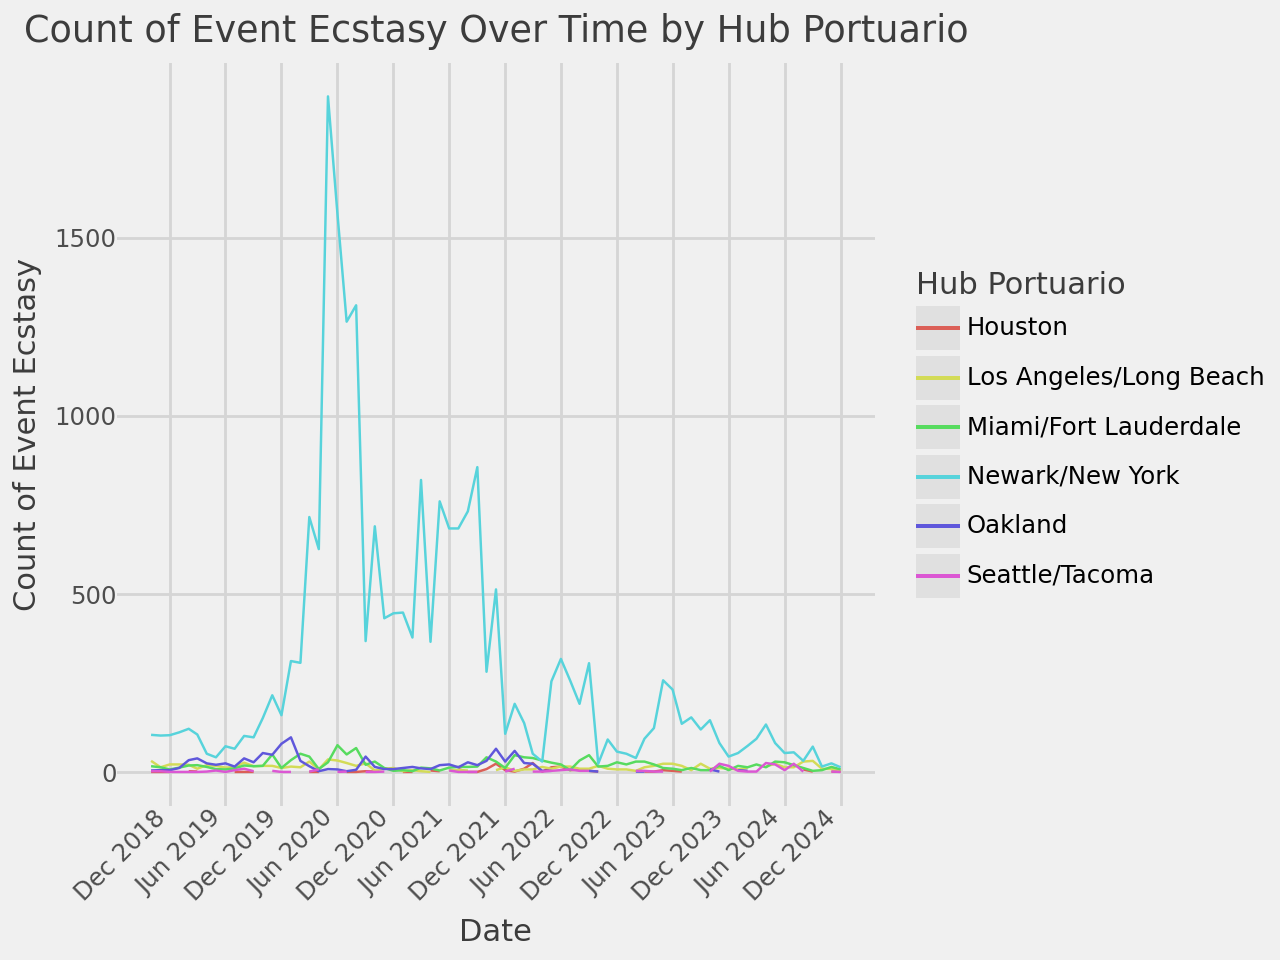
\includegraphics[width=0.8\textwidth]{timeseries_7.png}
		\end{figure}
	
		\begin{figure}[H]
			\caption{\label{timeseries_8} Redadas incautando heroína por puerto}
			\centering
			\hspace*{1cm}
			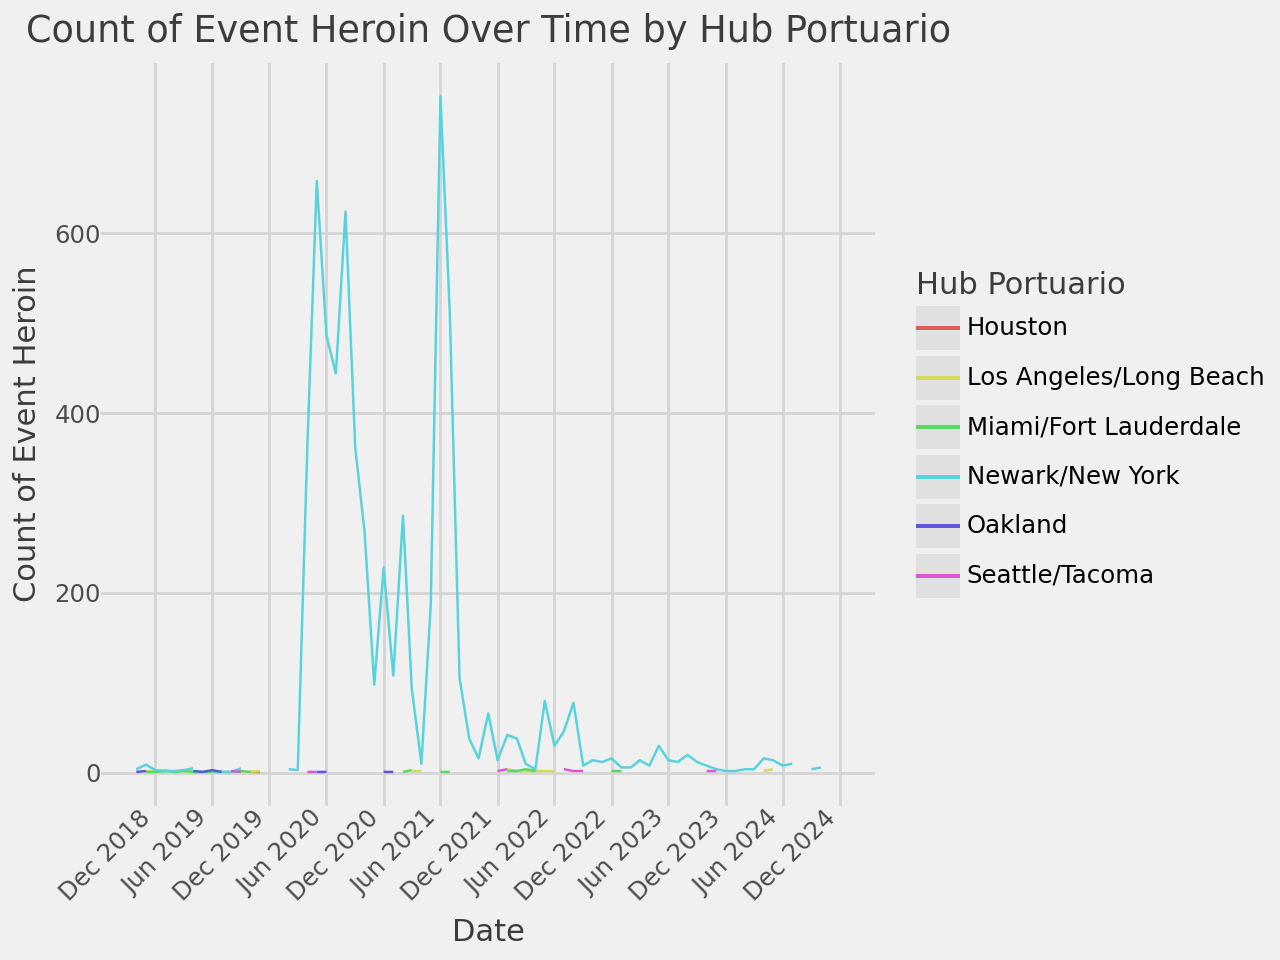
\includegraphics[width=0.8\textwidth]{timeseries_8.png}
		\end{figure}
	
		Sin embargo, si hay una categoría que resulta ser de la que más redadas hay es la considerada como "otras drogas" de las cuales no se especifica nada al respecto en los documentos originales. Véase la figura \ref{timeseries_9} también proporcionada en valores absolutos por puerto.
		
		\begin{figure}[H]
			\caption{\label{timeseries_9} Redadas incautando otras drogas por puerto}
			\centering
			\hspace*{1cm}
			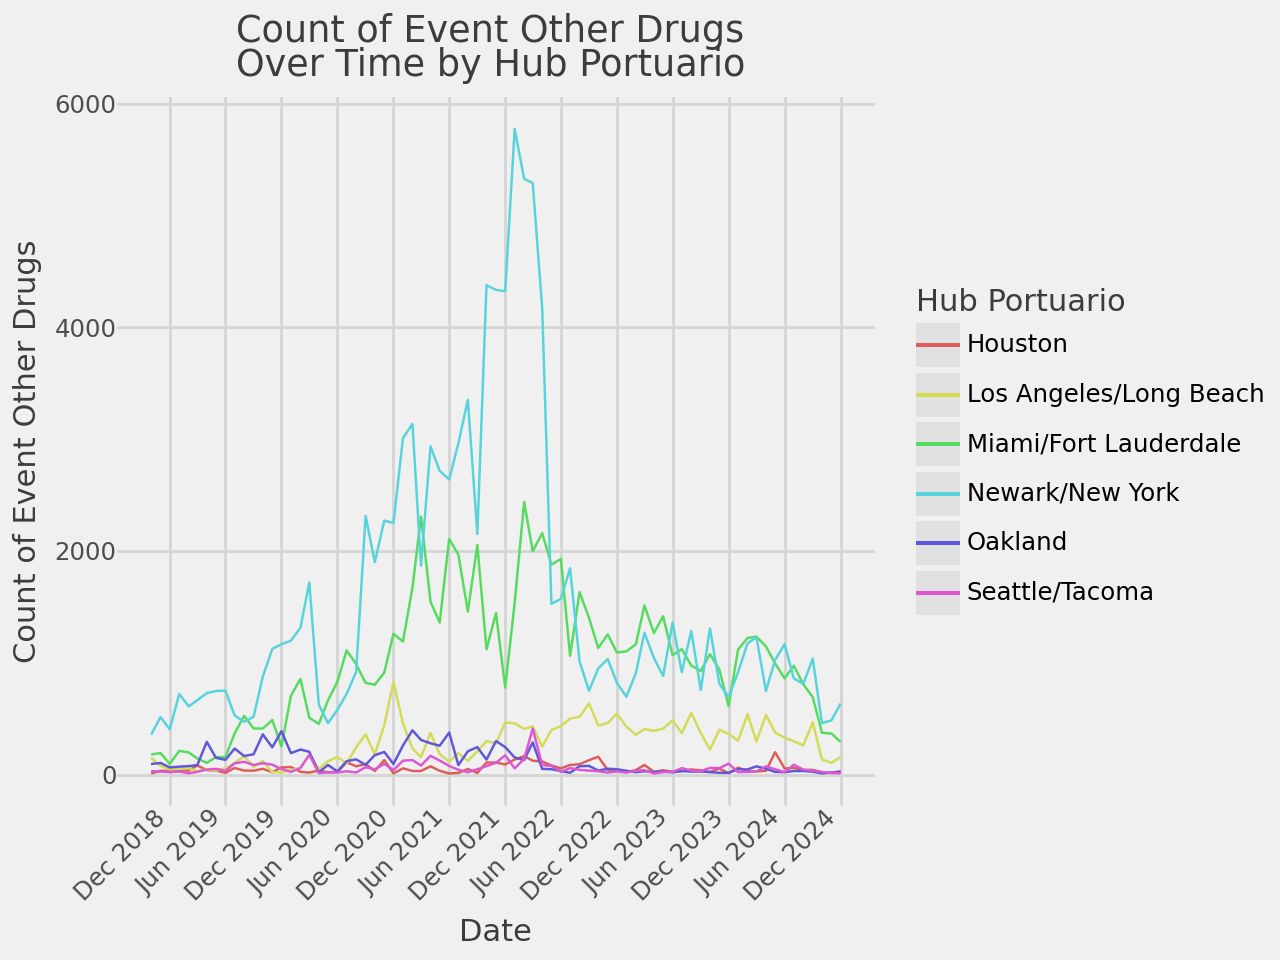
\includegraphics[width=0.8\textwidth]{timeseries_9.png}
		\end{figure}
	
		\underline{Análisis de Port Everglades}\\
		Port Everglades es como se conoce al puerto de Fort Lauderdale (en el hub portuario de Miami).
		
		Tras unas pequeñas demostraciones del comportamiento en función del tiempo de los distintos puertos, se tuvo en consideración la representación visual para variables respecto a este último puerto (véanse las figuras \ref{hist_1} y \ref{hist_2}). Nótese la estandarización de los datos para estas variables.
		
		\begin{figure}[H]
			\caption{\label{hist_1} Distribución por número de redadas por cada mes en Fort Lauderdale}
			\centering
			\hspace*{1cm}
			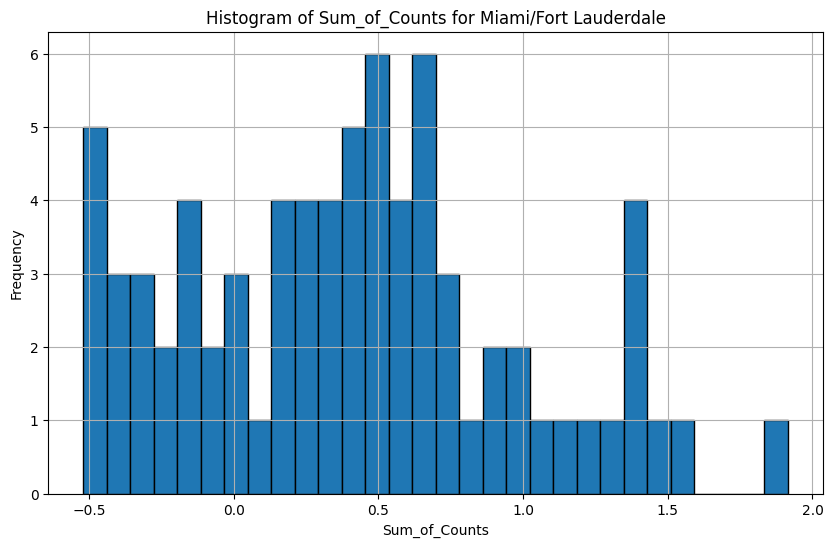
\includegraphics[width=0.8\textwidth]{hist_1.png}
		\end{figure}
	
		\begin{figure}[H]
			\caption{\label{hist_2} Distribución por número de TEUs por cada mes en Fort Lauderdale}
			\centering
			\hspace*{1cm}
			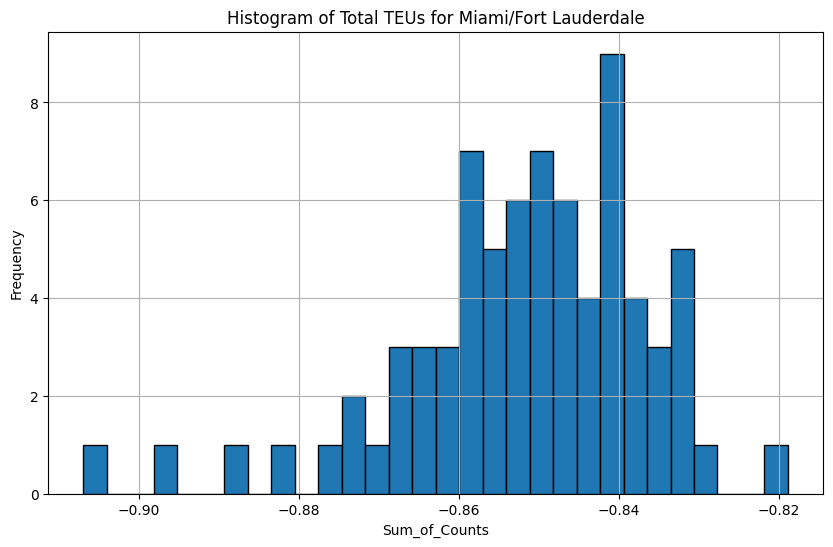
\includegraphics[width=0.8\textwidth]{hist_2.png}
		\end{figure}
	
		Por último, quiero destacar el perfecto comportamiento bimodal que se obtuvo del total de redadas del área metropolitana del Gran Los Ángeles (figura  \ref{hist_3})
		
		\begin{figure}[H]
			\caption{\label{hist_3} Distribución por número de redadas por cada mes en Los Ángeles}
			\centering
			\hspace*{1cm}
			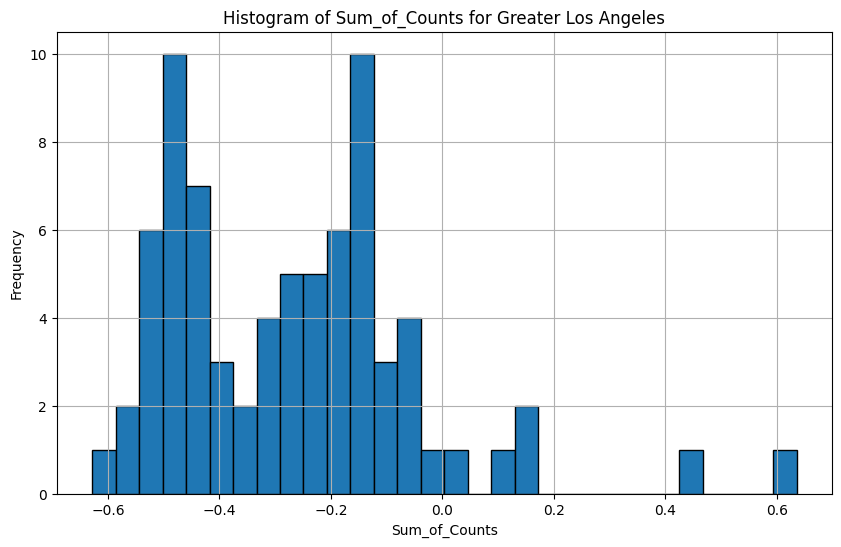
\includegraphics[width=0.8\textwidth]{hist_3.png}
		\end{figure}
	
		Es un caso a destacar por la forma de la distribución y, sobre todo, porque son datos obtenidos de la oficina de campo de Los Angeles (Los Angeles Field Office, \cite{cbp_la_field_office}) del CBP. Es decir, no se trata de una fusión de datos entre Los Ángeles y Long Beach que pudieran dar lugar a ello).
		
		
		\underline{Matrices de correlación de datos}\\
		Teniendo en cuenta que el propósito de este trabajo es generar un modelo que pudiese anticipar la droga incautada (sea la cantidad, el número de redadas, por tipo, etc) a partir de la actividad en un puerto (contenedores movilizados), resulta evidente generar una matriz de correlaciones para observar a primera vista si existía alguna variable que fuera fácilmente representante del "target". En las figuras \ref{matriz_corr_1} y \ref{matriz_corr_2} se muestra una relación entre las posibles variables predictoras y variables objetivo para los puertos de Newark y Fort Lauderdale, respectivamente.
		
		Realmente lo que se muestra en las figuras mencionadas en el párrafo anterior no representa la matriz de correlaciones per sé. Es un subconjunto menor en el que se enfrentan las variables de entrada (predictores, en el eje vertical) con alguno de los posibles targets para modelar (eje horizontal). Dada la baja correlación -salvo en contadas excepciones- entre las variables de contenedores y las de incautaciones de droga, a partir de aquí se empezará a ver lo complejo que es predecir la segunda (o el número de redadas) a partir de la actividad de la primera en un mismo mes. 
		
		\begin{figure}[H]
			\caption{\label{matriz_corr_1} Correlación entre variables predictoras y potenciales variables objetivo para el puerto de Newark}
			\centering
			\hspace*{1cm}
			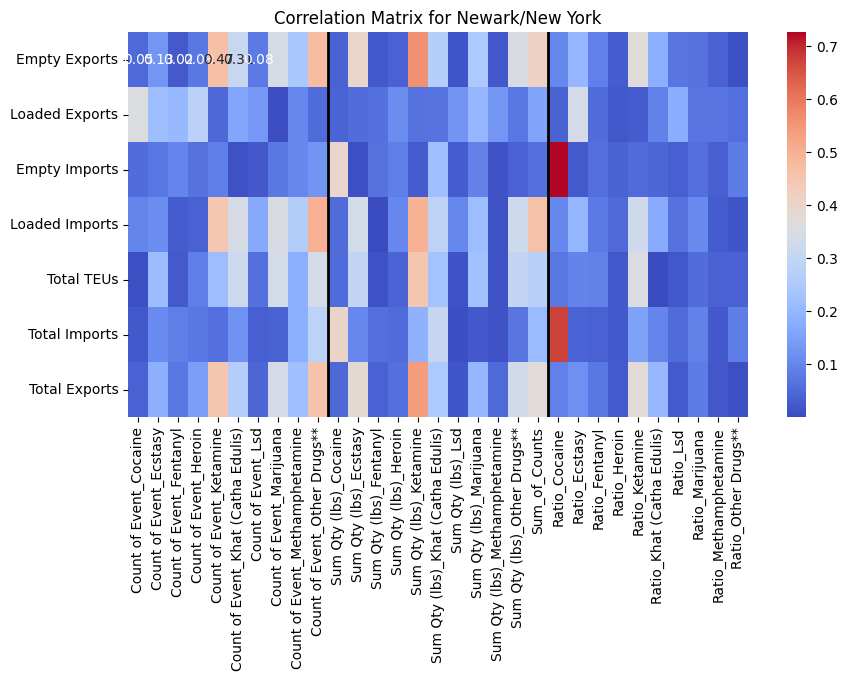
\includegraphics[width=0.8\textwidth]{matrix_corr_1.png}
		\end{figure}
	
		\begin{figure}[H]
			\caption{\label{matriz_corr_2} Para el puerto de Fort Lauderdale}
			\centering
			\hspace*{1cm}
			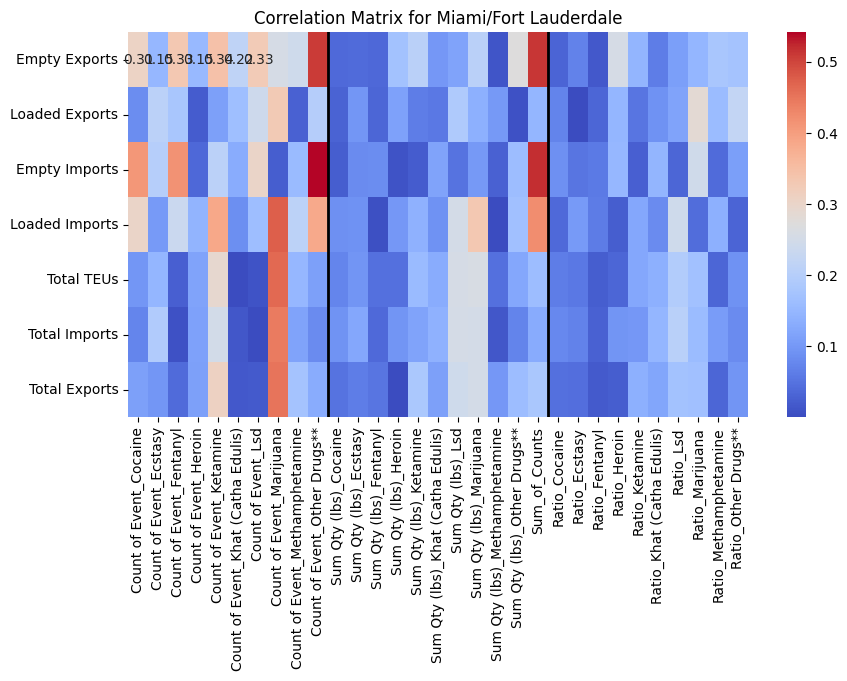
\includegraphics[width=0.8\textwidth]{matrix_corr_2.png}
		\end{figure}
		
		La figura \ref{matriz_corr_4} muestra un ejemplo de correlación entre variables predictoras para el caso del puerto de Newark (se ha comprobado que el comportamiento es muy similar para el resto de puertos. Ver la sección de anexos para matrices de correlación para otros puertos).
		
		\begin{figure}[H]
			\caption{\label{matriz_corr_4} Correlación entre predictores para el puerto de Newark}
			\centering
			\hspace*{1cm}
			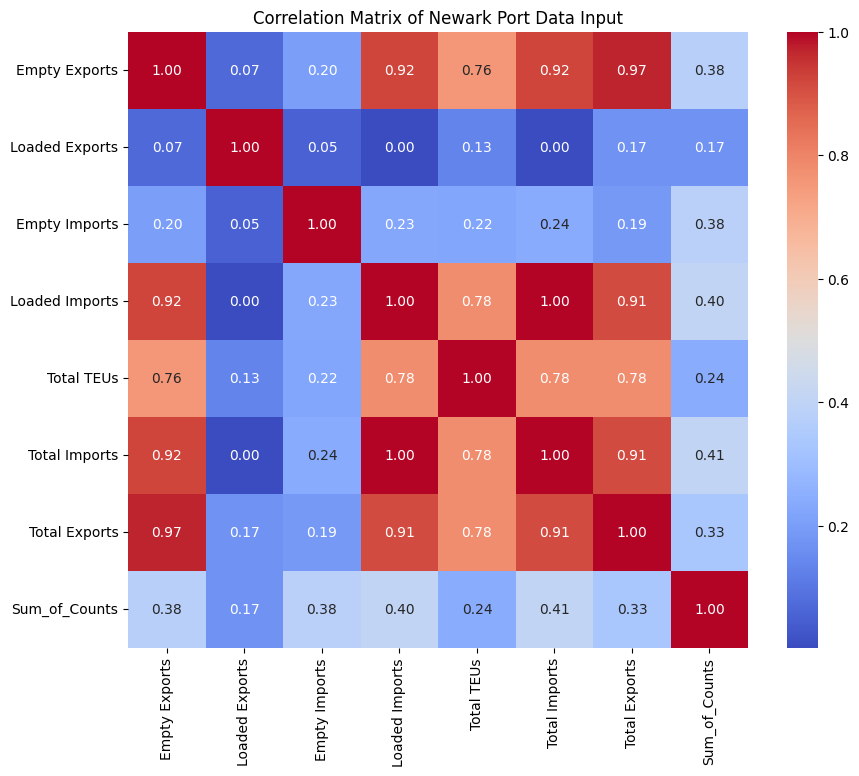
\includegraphics[width=0.7\textwidth]{matrix_corr_4.png}
		\end{figure}
	
		La lógica indica que la existencia de una fuerte correlación entre Total Imports y Loaded Imports viene dada por la naturaleza de las dos variables. No así con Total Exports que a pesar de todo, tiene una correlación con éstas mayor incluso que con Total TEUs. Seguramente sea una indicador del nivel de gestión de contenedores (en tiempo) sea muy alto. Es decir, los contenedores tarden muy poco en estar en la estiba o que, por otro lado, el nivel de actividad sea tal que el resultado neto es que entren tantos contenedores (importaciones) como salgan del puerto (exportaciones). Dicho sea de paso, el concepto "exportaciones" no se aclara si son salidas del puerto por vía marítima o terrestre (interior, inland en inglés). De todos modos, en caso de tener que prescindir de variables (debido a la redundancia entre éstas) serían las de exportaciones. Tiene más sentido desarrollar un modelo que prediga la cantidad de droga (a partir de los datos de incautaciones) que entra en un puerto, dados los datos de importaciones.
		
		
		Dada la poca claridad respecto a la finalidad del problema, se llegó a plantear distintos enfoques a distintos niveles. Es decir, se barajó un modelo para un puerto en concreto, para varios puertos por separado o con todos a la vez. Considerando o no sus variables geográficas, qué tipo de droga analizar. Todo ello ha sido recopilado a lo largo de esta subsección que concluye con una pequeña amalgama de mapas y otras visualizaciones.
		
		Por ejemplo, se estudió variación temporal del total de contenedores gestionados por cada puerto \ref{total_teus_ports}, junto con la cantidad de contenedores vacíos (y cargados) \ref{loaded_vs_imports_ports} gestionados por los mismos.
		
		\begin{figure}[H]
			\caption{\label{total_teus_ports} Serie temporal con TEUs gestionados por los puertos}
			\centering
			\hspace*{1cm}
			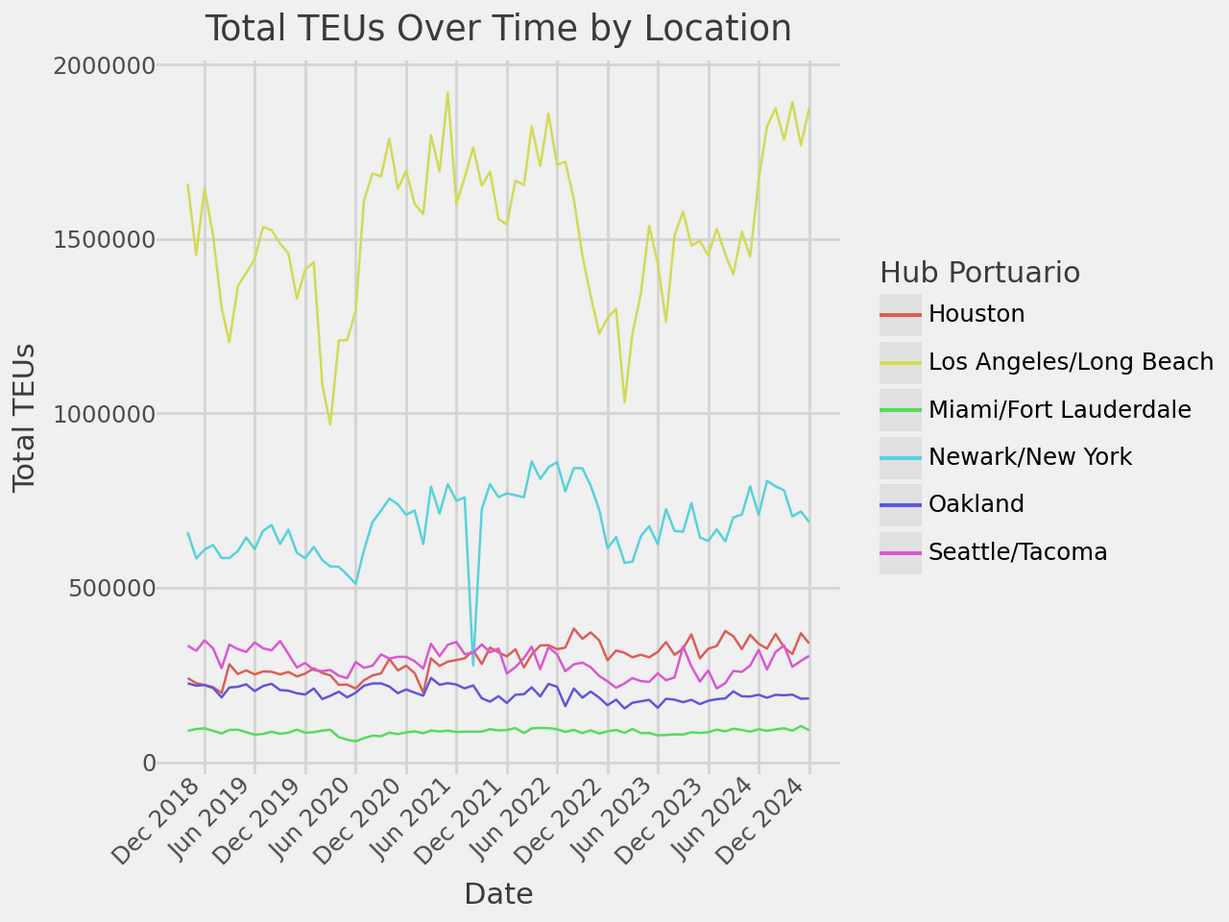
\includegraphics[width=0.8\textwidth]{total_teus_ports.png}
		\end{figure}
		
		
		\underline{Mapas geográficos}\\
		Debido a ciertos problemas a la hora de visualizar en un mapa los gráficos de tipo pie chart, se renunció a ello. La separación entre los gráficos \ref{loaded_vs_imports_ports} y \ref{map_bubble_1} viene a dar cuenta de ello.
		
		\begin{figure}[H]
			\caption{\label{loaded_vs_imports_ports} Contenedores gestionados por puertos por tipo: Vacío o Cargado}
			\centering
			\hspace*{1cm}
			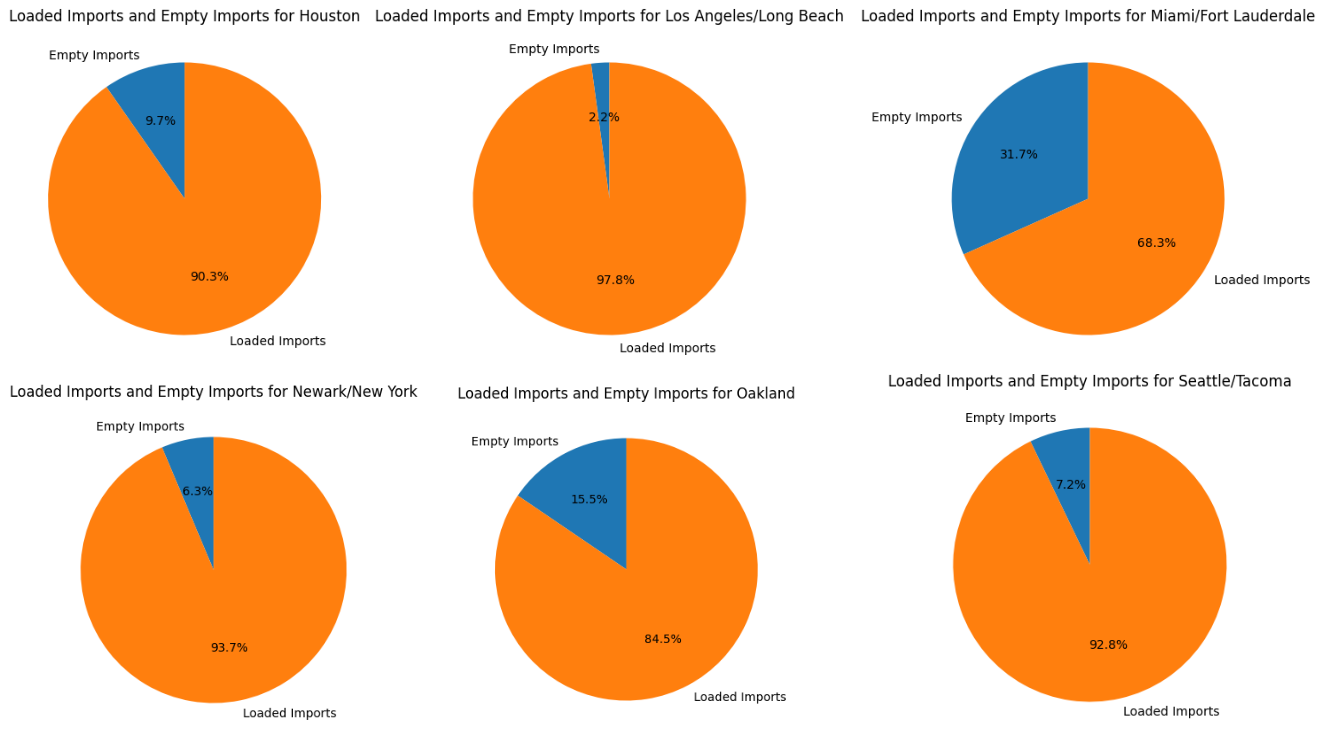
\includegraphics[width=0.8\textwidth]{loaded_vs_imports_ports.png}
		\end{figure}
	
		
		\begin{figure}[H]
			\caption{\label{map_bubble_1} }
			\centering
			\hspace*{1cm}
			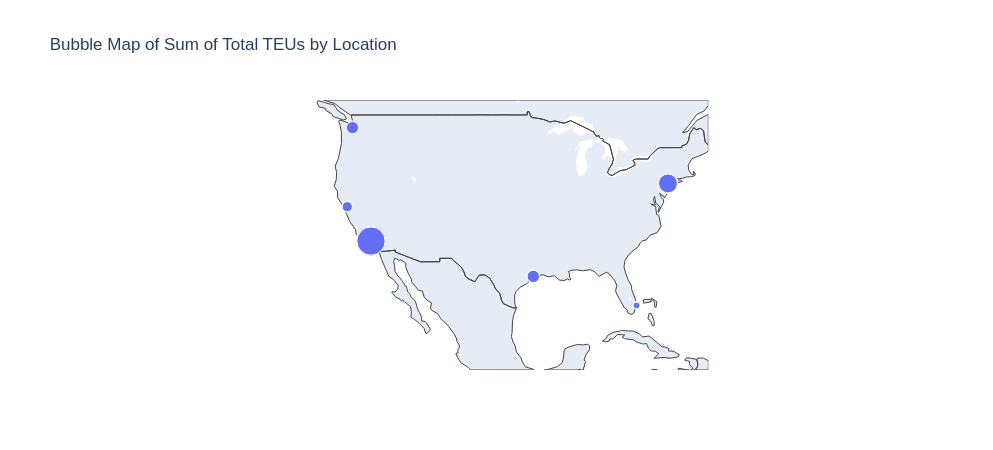
\includegraphics[width=\textwidth]{map_bubble_1.png}
		\end{figure}
	
		Nótese que el puerto de Fort Lauderdale es el que tiene mayor cantidad de contenedores vacíos (por encima del 30\%). Sin embargo, en términos totales de volumen gestionado es el menor de todos los investigados. Y como se comentó en apartados anteriores, los puertos del área metropolitana del Gran Los Ángeles son los que más actividad tienen, seguidos por el puerto de Newark en Nueva Jersey. También, añadir que el puerto de Los Ángeles es el que menos contenedores vacíos importa, sumado esto a su alta operabilidad.

		Pese a lo comentado anteriormente, si que se puede realizar un análisis de la situación de los puertos con más actividad (Los Ángeles a la cabeza), al igual que, como se irá viendo a continuación, hacerlo para cada tipo de droga y cada puerto.
		
		\begin{figure}[H]
			\caption{\label{map_bubble_2} }
			\centering
			\hspace*{1cm}
			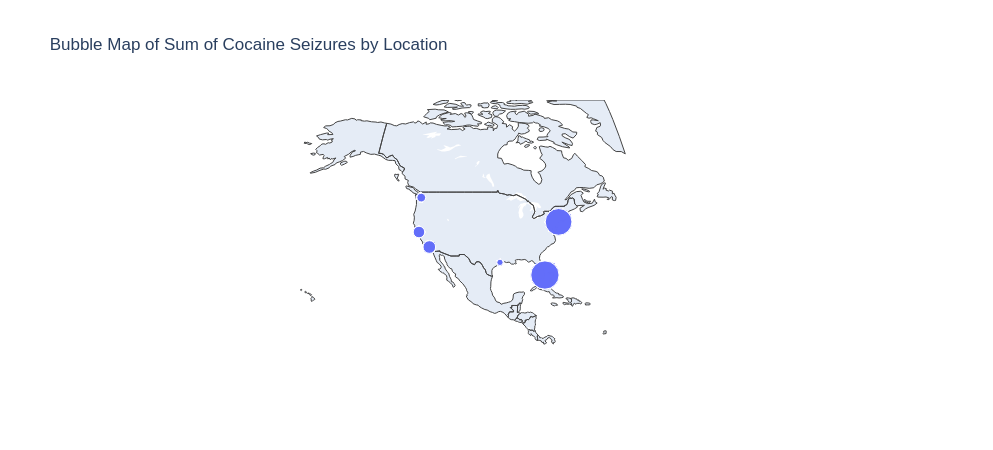
\includegraphics[width=\textwidth]{map_bubble_2.png}
		\end{figure}
	
		\begin{figure}[H]
			\caption{\label{map_bubble_3} }
			\centering
			\hspace*{1cm}
			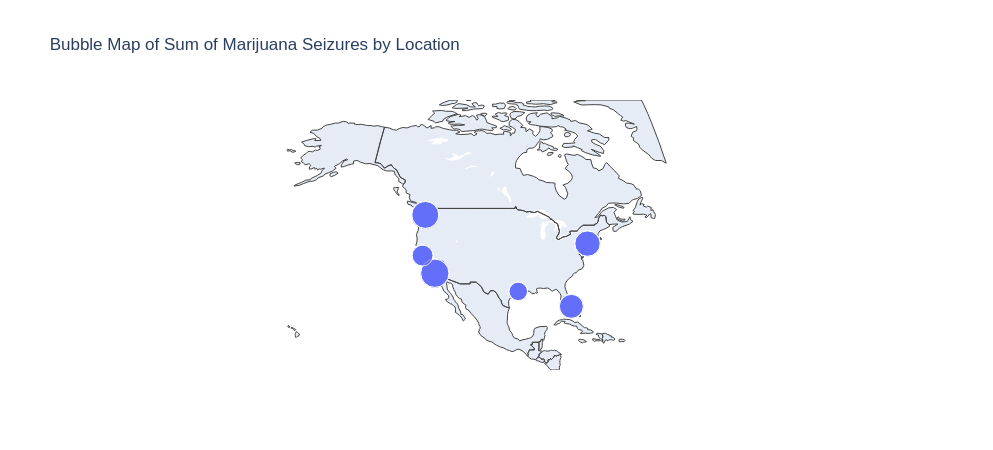
\includegraphics[width=\textwidth]{map_bubble_3.png}
		\end{figure}
	
		\begin{figure}[H]
			\caption{\label{map_bubble_4} }
			\centering
			\hspace*{1cm}
			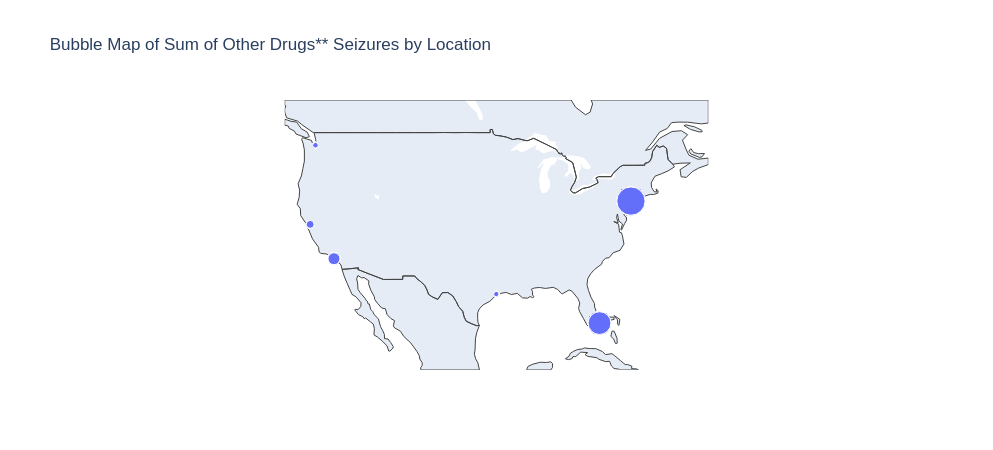
\includegraphics[width=\textwidth]{map_bubble_4.png}
		\end{figure}
	
		Por ejemplo, en las figuras \ref{map_bubble_2}, \ref{map_bubble_3} y \ref{map_bubble_4} se muestran el total de incautaciones para cocaína, marihuana* y otras drogas (no especificadas) incautadas para cada puerto. Se pueden relacionar estos tres mapas con las series temporales de \ref{timeseries_6} para el caso de la cocaína o  \ref{timeseries_9} para el caso de otras drogas, respectivamente.
		
		El puerto de Newark/Nueva York es un ejemplo paradigmático sobre incautaciones frecuentes para todos los tipos de drogas. La cocaína se incauta más en la zona de la costa este (especialmente por Miami) al igual que "Other Drugs". Seguramente conocer la distribución del origen geográfico de las importaciones habría aportado más información a este trabajo. Sin embargo, atendiendo a la figura \ref{timeseries_6}, anteriormente mostrada, la comparación con el número de redadas era considerablemente menor que en otros casos (Véanse \ref{timeseries_7} o \ref{timeseries_8}). Especialmente para el caso de Newark.
		
		\begin{figure}[H]
			\caption{\label{map_bubble_6} }
			\centering
			\hspace*{1cm}
			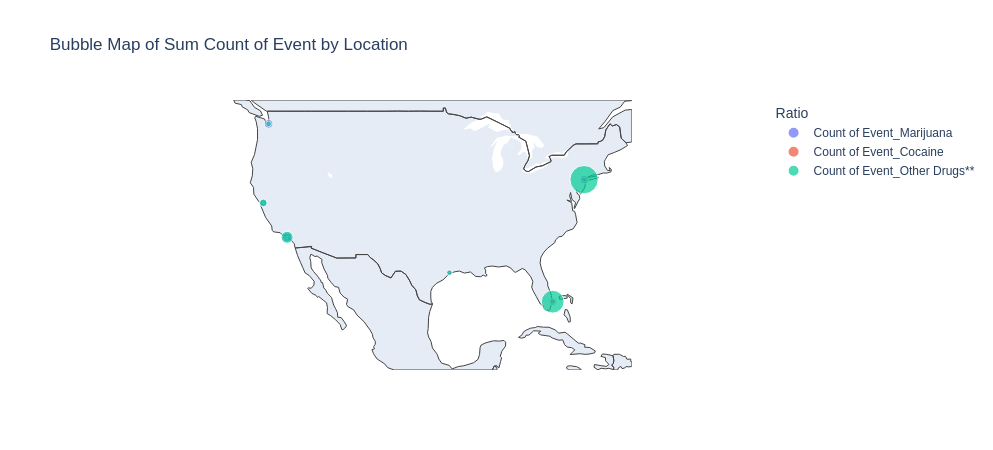
\includegraphics[width=\textwidth]{map_bubble_6.png}
		\end{figure}
		
		Por ejemplo, en la figura \ref{map_bubble_6} se muestra la cantidad de redadas por puerto para las tres principales drogas: cocaína, marihuana y otras. En todos los puertos las principales incautaciones hacen referencia a "otras", excepto para el hub portuario Seattle/Tacoma que lo hacen para marihuana. Eso sí, si observamos el radio de las burbujas del gráfico, en Seattle es muy residual.
		
		
		% Incluir pie de página para remarcar que la marihuana está legalizada en ciertos estados como California o Washington.
		
		\subsubsection{\label{preprocessing}Pre-procesamiento de los datos}
		% Limpieza, Tratamiento de Missing Values, Normalización, Estandarización, Tratamiento de Outliers...
		Este primer dataset construido, consta de 31 variables: Date (formato fecha 'YYYY-mm'), latitud y longitud (numérico float64), siete variables numéricas correspondientes a los datos portuarios, el resto de variables corresponden a los datos de incautaciones de drogas: diez variables numérica sobre "número de eventos" por droga o "Count of Events" en la versión original más una variable sumatoria de estas diez "Sum of Counts" y otras diez sobre la cantidad (en libras) incautada por droga.
		
		% Codigo con columnas del dataset
		
		\underline{Aplicaciones de scikit-learn}\\
		A la vista del primer análisis exploratorio de datos, se encontraron missing values en las variables relacionadas con las incautaciones de drogas y una gran diferencia de escala entre los datos portuarios (centenas de miles de contenedores) frente a los datos de incautaciones (decenas de incautaciones). Los missing values, al tratarse de datos de fuentes de origen fiables, se imputaron a cero haciendo uso de la función SimpleImputer provista por la librería de scikit-learn. En ese caso, se consideró que durante aquel mes para aquella oficina de campo aduanera, no hubo incautación. Para seguir por esa línea, se observó una determinada constancia en la ausencia de datos en los pares número de incautaciones-cantidad incautada. Es decir, se comprobó que si no había datos de incautación, no había datos de cantidad incautada y, por tanto, se imputase a cero. Entendible todo ello en el contexto de que se considerase de que no hubo redada (al menos exitosa en relación a esa droga). Por su parte, para la normalización de datos se aplicó la función StandardScaler también proporcionada por scikit-learn. Es a partir de aquí, que los datos con los que se van a trabajar están estandarizados a media cero y varianza uno.
		
		\underline{Detalles del pipeline de scikit-learn}\\
		Dado que los rangos para variables de distinto tipo (incautaciones vs contenedores) eran muy diferentes entre sí, se procedió a la estandarización de los mismos mediante la implementación de pipelines en scikit-learn. Los datos numéricos ausentes se imputaron a cero (como se explicó en el párrafo anterior) y se estandarizó a una normal(0,1). Por su parte, las variables categóricas se dispusieron a ser tratadas mediante 'OrdinalEncoder'*.
		
		% Incluir fragmento de código del Pipeline scikit-learn
		\begin{verbatim}
			from sklearn.impute import SimpleImputer
			from sklearn.preprocessing import StandardScaler, OrdinalEncoder
			from sklearn.pipeline import FeatureUnion, Pipeline
			from sklearn.compose import ColumnTransformer
			
			numeric_columns = combined_data.select_dtypes(include=['float64']).columns
			date = combined_data['Date']
			
			# Define the pipeline
			# Define the transformers for numeric and categorical columns
			numeric_transformer = Pipeline(steps=[
			('imputer', SimpleImputer(strategy='constant', fill_value=0)),
			('scaler', StandardScaler())
			])
			
			categorical_transformer = Pipeline(steps=[
			('ordinal_encoder', OrdinalEncoder())
			])
			
			# Combine transformers using ColumnTransformer
			preprocessor = ColumnTransformer(
			transformers=[
			('num', numeric_transformer, numeric_columns),
			('cat', categorical_transformer, ['Hub Portuario'])
			]
			)
			
			# Define the final pipeline
			pipeline = Pipeline(steps=[
			('preprocessor', preprocessor)
			])
			
			# Apply the pipeline to the numeric columns
			standardized_data = combined_data.copy()
			standardized_data = pipeline.fit_transform(standardized_data)
		\end{verbatim}
	
		Uno de los casos de evitar el uso de One-Hot-Encoder se basó en la poca optimización de los recursos de memoria (aunque en este caso fuera anecdótico) frente a alternativas como OrdinalEncoder o TargetEncoder. En otras palabras, en vez de crear N variables nuevas por cada caso distinto de la variable categórica original, se mantiene una variable con los datos categóricos numerizados.
		
		Otro aspecto a remarcar en el proceso de estandarización de los datos fue que esa estandarización se produjo con el dataset para los distintos puertos integrados. Es por ello que en algunas gráficas mostradas, para un hub portuario en particular, se ven que las distribuciones de los datos se encuentran un poco alejadas de lo que debería ser su media (cero). También esto sirve para comparar el peso que tiene cada puerto o cada tipo de droga respecto del resto.
		
		\underline{Error original en los datos de Los Angeles}\\
		En el caso de los datos obtenidos del puerto de Los Ángeles, se detectó un error de formato en los datos de origen. En efecto, para el dato del mes de noviembre del 2020 (año fiscal 2021, \cite{portla2025containerstats}) se verificó un error respecto al formato de separador de miles (coma vs punto) en la columna 'Total TEUs'. Dado que se verificó que esta columna era igual a la suma de los valores de las columnas 'Total Imports' and 'Total Exports', se aplicó la suma de esos valores para la observación del mes de noviembre de 2020.
		
		\underline{Datos en miles para el puerto de Newark}\\
		Por su parte, resultó que los datos obtenidos para el puerto de Newark (Área Metropolitana de Nueva York-Nueva Jersey) estaban contados en miles (de contenedores). Para resolverlo, se multiplicaron estos valores por mil aparte del resto de datos para después, ser reintegrados \cite{panynj2025facts}. Posiblemente el problema de integración se tratase de una incompatibilidad entre el formato europeo y americano de separador de miles.
		
		\underline{Missing Values en los datos de Fort Lauderdale}\\
		Por su parte, como se mencionó en la sección \ref{data origin}, en el caso de Fort Lauderdale, debido a las características particulares de su adquisición e integración de datos, se observaron la falta de los mismos correspondientes al último trimestre del año fiscal 2021.
		
		% Captura de pantalla para 2021 FY.
		
		Una ventaja que se tenía a la hora de poder imputar estos datos, era la posesión de todos los datos de años fiscales a nivel anual, es decir, el valor integrado de los datos mensuales \cite{waterborne2024commerce}. Conociendo estos datos y dado que no solo ofrecían el total de contenedores o de importaciones/exportaciones sino también qué contenedores están cargados y cuáles están vacíos, se pudo plantear el problema de la imputación de los missing values como valores MNAR, es decir, imputarlos a partir del contexto. Se aseguró que realmente los datos anuales coincidían con los datos mensuales y, en consecuencia, se fueron imputando según variables: de Loaded Imports, a Empty Exports, así hasta el total de importaciones y de exportaciones y, en último lugar, el total de TEUs (suma de las dos variables previas). En último lugar, respecto a esta operación, se imputó el mismo valor para cada mes ausente (una alternativa que se planteó fue la imputación aleatoria con una media próxima al valor imputado pero una cierta varianza incluida, es decir, generando un poco de ruido).
		
		A continuación se muestra un pequeño fragmento de código para la imputación de los missing values en la variable "Loaded Imports":
		
		\begin{verbatim}
			# Compute proportions
			prop_imports = data['Loaded Imports'].sum(skipna=True) / (data['Loaded Imports'].
					sum(skipna=True) + data['Loaded Exports'].sum(skipna=True))
					
			prop_exports = 1 - prop_imports
			
			# Compute missing values
			missing_total = 186169
			impute_value_imports = round((missing_total * prop_imports)/data['Loaded Imports'].isna().
			sum())
			
			impute_value_exports = round((missing_total * prop_exports)/data['Loaded Exports'].isna().
			sum())
			
			# Impute missing values
			data.loc[data['Loaded Imports'].isna(), 'Loaded Imports'] = impute_value_imports
			data.loc[data['Loaded Exports'].isna(), 'Loaded Exports'] = impute_value_exports
		\end{verbatim}
	
		Este proceso se generalizó para el resto de variables con missing values para el puerto de Fort Lauderdale. Con esto se trató el principal problema de missing values que, como se mencionó al principio del trabajo, no fue la tónica general. Los informes, tablas y fuentes de datos eran de calidad en ese aspecto.
		
		\underline{Tratamiento de outliers}\\
		Para el tratamiento de outliers, en un primer momento se fue estudiando caso a caso, la situación de cada uno, su contexto, etc. Intentando comprender qué valor aportaba al modelo, si pudiera ser un dato que alterase en exceso al resto o si fueran datos que simplemente estuviesen un poco más allá de las fronteras teóricas (rango intercuartil, QQ-Plot, método de las tres sigmas) fuera de lugar.
		Dado que el número de observaciones no era demasiado grande, en muchos casos, se limitó a que el umbral para excluir datos fueran criterios muy alejados en las colas de la distribución tales como el valor absoluto cinco de los datos normalizados. Es decir, se intentó minimizar el número de datos excluidos, pero se decidió que en algunos casos, eran necesarios para avanzar en el estudio del problema.
		
		En la siguiente sección \ref{feature engineering} se hace referencia y se detalla la generación de nuevas variables. Entre ellas destaca el conjunto de variables de tipo "Ratio". Pese a no haberse hecho mención de ella, salvo si acaso, de pasada, será útil para detectar ciertas anomalías en los comportamientos. Esto puede servir para ver como orientar el modelo, más allá de que se acabe usando o no en éste. Aportará información de gran relevancia de forma visual. Aquí dejo una serie de gráficas estandarizadas sobre esa variable que sirve para detectar ciertos valores extremos (outliers) que serán excluidos.
		
		
		% Visualización (o datos) de media por hub portuario de incautaciones y de tráfico de contenedores.
		
		El criterio de exclusión de outliers ha sido muy laxo. Como se ha mencionado en uno de los párrafos anteriores, se han considerado todos aquellos valores normalizados más allá de cinco, por ejemplo. Esto es debido a la escasez de datos y con la intención de minimizar el número de datos a excluir, buscando aquellos valores que se encontrasen en los extremos residuales de las colas de la distribución normal.
		
		% [Tras eliminar outliers] Graficos de dispersion (scatter plots). Correlacion entre variables.
		\begin{figure}[H]
			\caption{\label{boxplot_1} Boxplot para hallar outliers en redadas de cocaína}
			\centering
			\hspace*{1cm}
			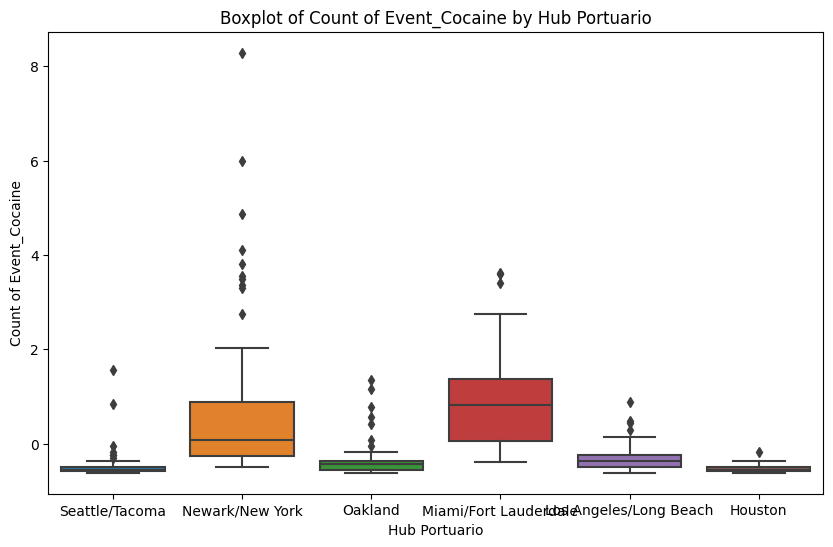
\includegraphics[width=\textwidth]{boxplot_1.png}
		\end{figure}
	
		\begin{figure}[H]
			\caption{\label{boxplot_3} Boxplot para hallar outliers en ratios de cocaína}
			\centering
			\hspace*{1cm}
			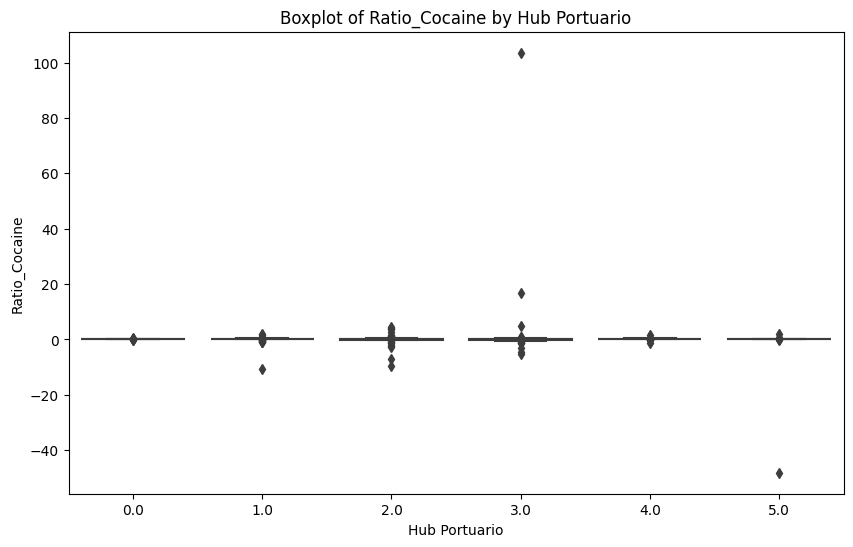
\includegraphics[width=\textwidth]{boxplot_3.png}
		\end{figure}
	
		\begin{figure}[H]
			\caption{\label{boxplot_4} Boxplot para hallar outliers en redadas de otras drogas}
			\centering
			\hspace*{1cm}
			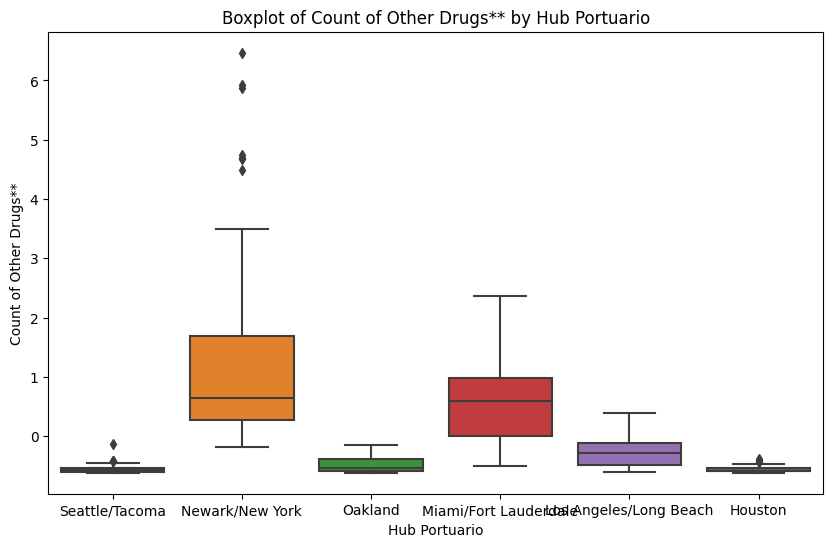
\includegraphics[width=\textwidth]{boxplot_4.png}
		\end{figure}
	
		\begin{figure}[H]
			\caption{\label{boxplot_2} Boxplot para hallar outliers en ratios de otras drogas}
			\centering
			\hspace*{1cm}
			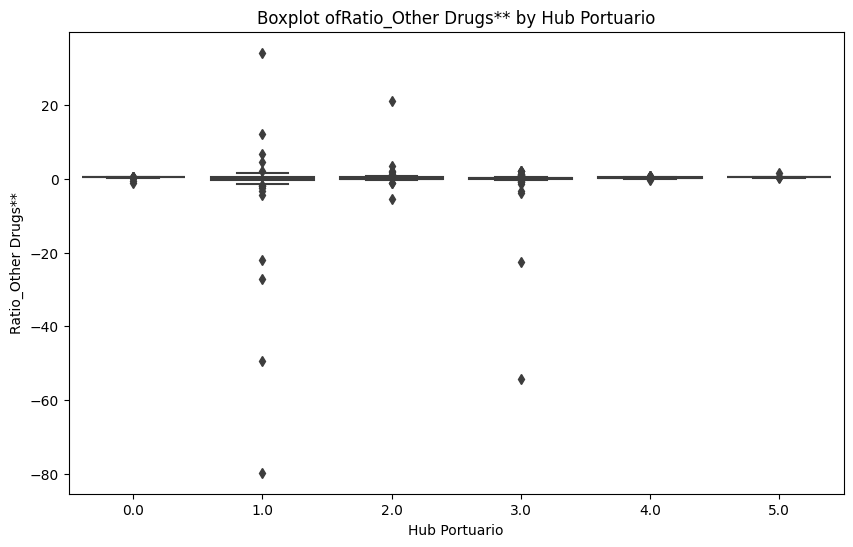
\includegraphics[width=\textwidth]{boxplot_2.png}
		\end{figure}
	
		Obsérvese en qué valores se sitúan aquellos referentes a las variables "Ratio", muy alejados del resto del grupo de valores. En cambio, para las variables "Count" la distribución es más común y aquellos valores outliers no afectan tanto a la distribución. Y aunque estrictamente, algunos valores de los boxplots para las variables que no son "Ratio" superen ese valor de cinco (con la distribución estandarizada), se ha decidido mantenerlos. Es decir, un criterio secundario ha sido observar como de alejado está un dato concreto respecto de otro par (distancia entre puntos).
	
		En los pares de imágenes \ref{boxplot_1} - \ref{boxplot_3}  y \ref{boxplot_4} - \ref{boxplot_2} se muestra que la aplicación de la variable ratio tenderá a poseer datos que se alejan mucho del resto. Éstos podrían considerarse como grandes redadas, grandes operaciones de incautación de una tacada. Ello hace que algunos puertos con poca actividad ilícita detectada, tenga algunos meses especiales que sobresalgan respecto a su media. A continuación se dejan algunas visualizaciones temporales para distintos puertos en los que se observan este tipo de comportamientos.
	
		Por ejemplo, obsérvese que para el caso de redadas de cocaína, se tiene constancia de una redada a principios de 2023 en Seattle con una gran cantidad de la misma incautada \ref{st_ratio_1}. En el caso de trabajar con esta variable "ratio cocaine", se vería que, en efecto, para el caso de Seattle hubo una importante operación en la que se incautó una gran cantidad de cocaína. El resto de valores se encuentran muy próximos de la media.
		
		\begin{figure}[H]
			\caption{\label{st_ratio_1} Serie temporal sobre redadas de cocaína para cada puerto}
			\centering
			\hspace*{1cm}
			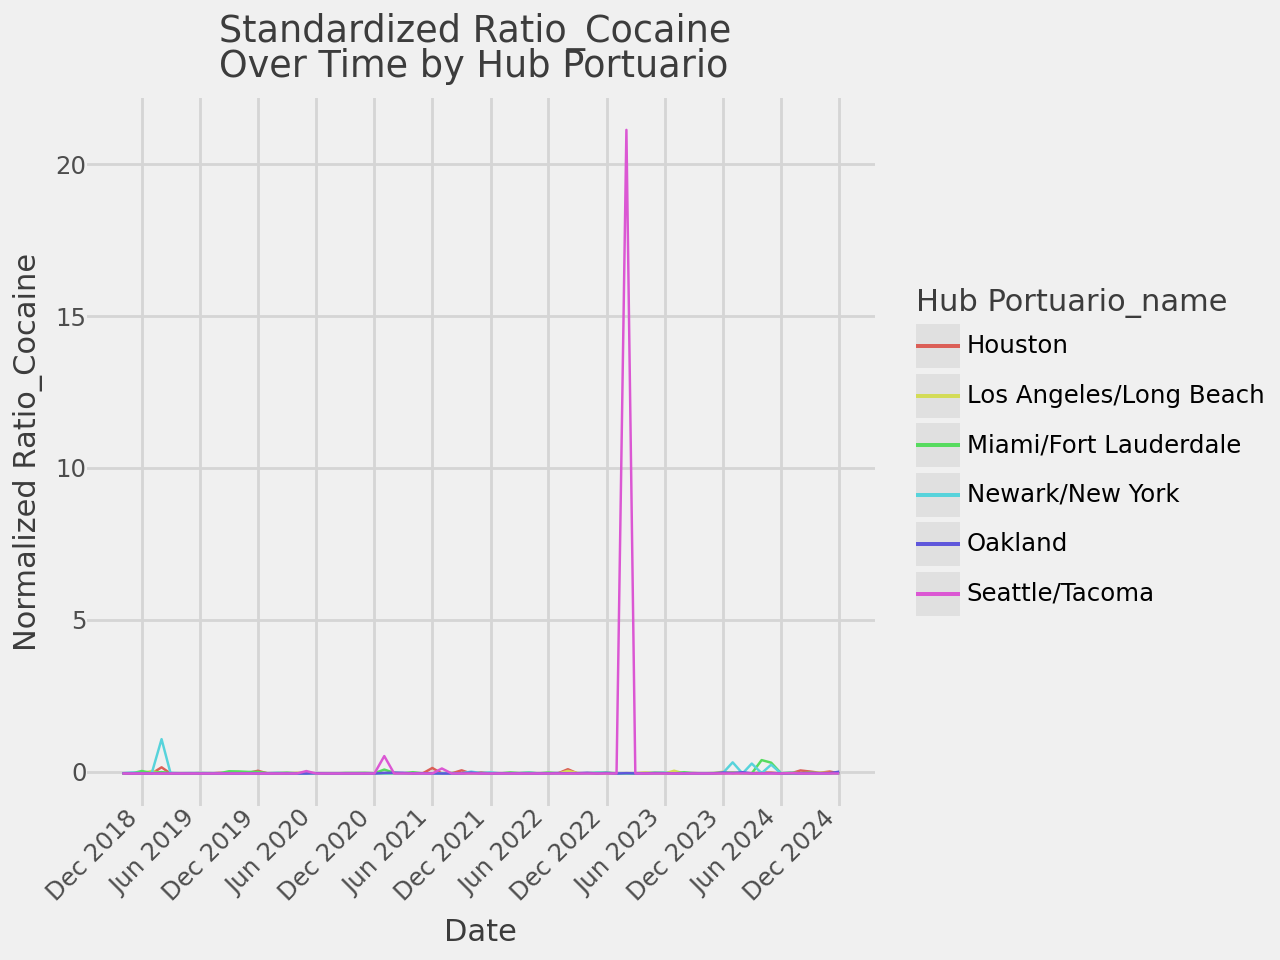
\includegraphics[width=0.75\textwidth]{st_ratios_1.png}
		\end{figure}
	
		En el caso de redadas de marihuana \ref{st_ratio_2}, se observan grandes redadas realizadas por las distintas oficinas de campo cada cierto tiempo. Pese a tratarse de una droga de consumo legal en ciertos estados (entre ellos California o el estado de Washington), ésta se incluye en los informes del CBP sin detallar si es de contrabando o cuál es su status real. En este trabajo no se entra a detallar el status, más allá de que vengan incluidas en las estadísticas mensuales aportadas. Curiosamente se observa que en el puerto de Los Angeles se realizan las redadas con mayor cantidad de marihuana incautada.
		
		\begin{figure}[H]
			\caption{\label{st_ratio_2} Serie temporal sobre redadas de marihuana para cada puerto}
			\centering
			\hspace*{1cm}
			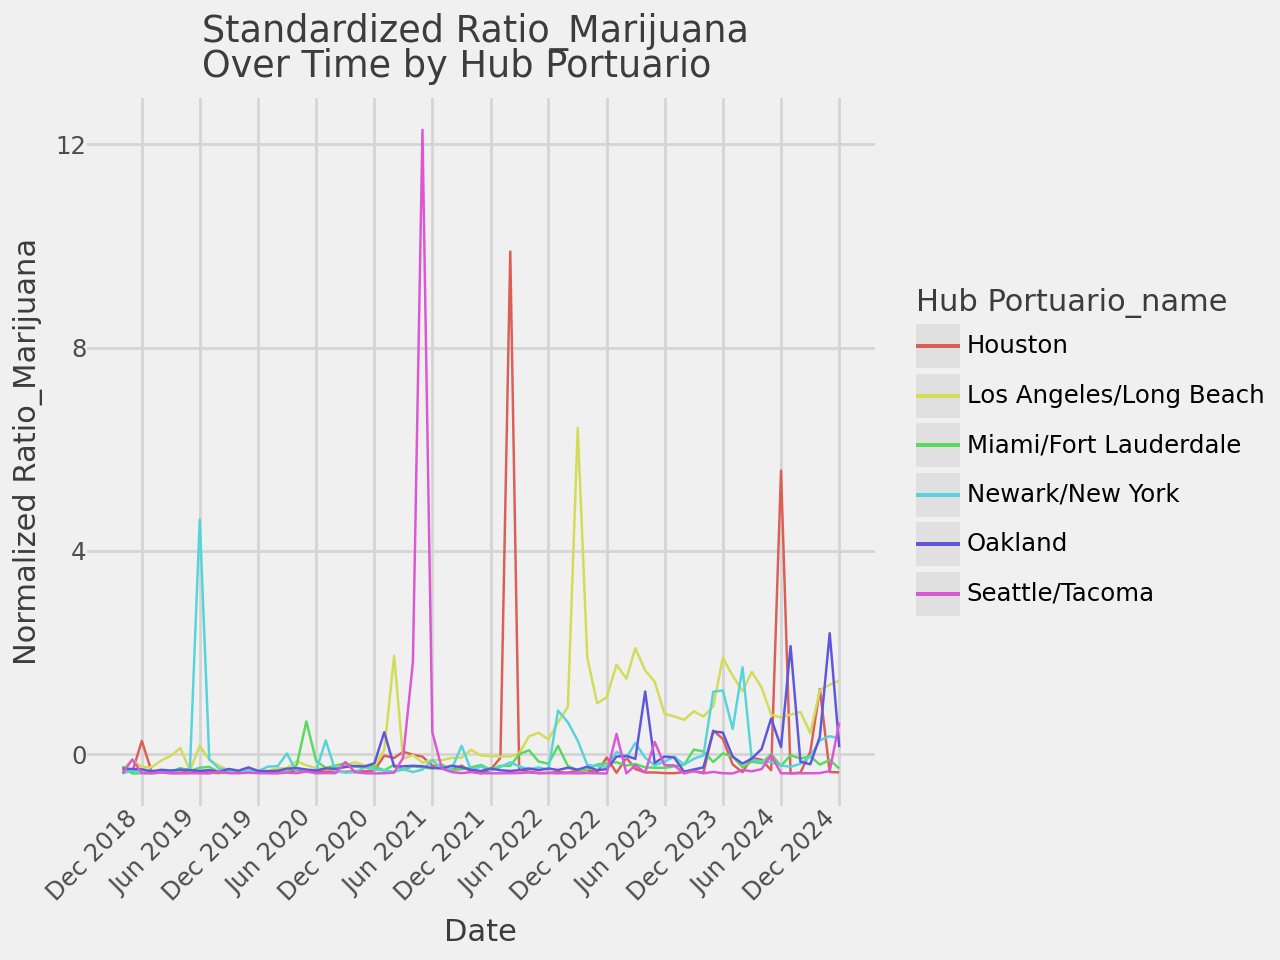
\includegraphics[width=0.75\textwidth]{st_ratios_2.png}
		\end{figure}
	
	
		\underline{Ejemplo de outlier en GLA}\\
		También se muestra el comportamiento para las redadas de "Otro tipo de drogas" (Véase la figura \ref{st_ratio_3}). En este caso destaca una redada importante en el hub portuario del Gran Los Ángeles (GLA)
		
		\begin{figure}[H]
			\caption{\label{st_ratio_3} Serie temporal sobre redadas de otro tipo de drogas para cada puerto}
			\centering
			\hspace*{1cm}
			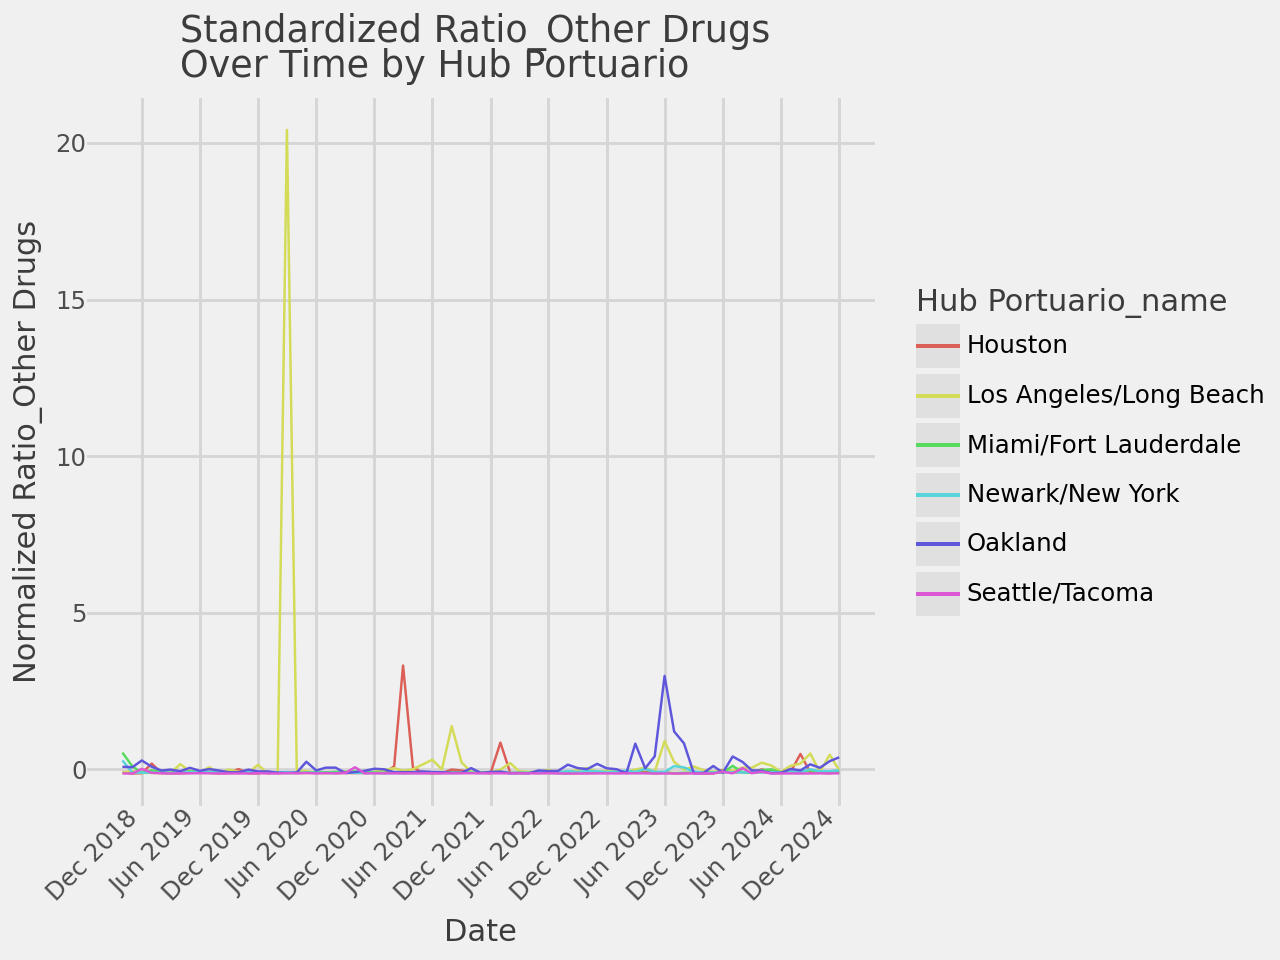
\includegraphics[width=0.7\textwidth]{st_ratios_3.png}
		\end{figure}
	
		Este caso particular va a servir para mostrar la alteración del dataframe tras el tratamiento de la observación con este outlier.
		
		\underline{Tratamiento de outliers para puerto de Newark}\\
		Por su parte, realizando un análisis exploratorio de datos para los datos referentes al puerto de Newark/Nueva York, se descubrieron ciertos valores anómalos. Los gráficos qq-plot que se muestran a continuación dan cuenta de ello (Ver figuras \ref{qqplots_1} y \ref{qqplots_2}).
		
		En efecto, se detectó que para dos variables concretas, muy relacionadas la una con la otra, había dos datos que se alejaban de la distribución para el resto de datos. Para estos dos valores detectados se da la condición de que representan valores registrados durante los meses de febrero de 2019 y 2022. No se halla ninguna otra relación aparente con el resto de meses o años para el mismo puerto. Y del resto de variables, no hay ninguna otra que sobresalga como aquí lo hacen.
		
		Como se verá más adelante, para asegurarse el valor que pudieran aportar estos datos a otras variables, se van a comparar con el resto de potenciales variables target en diagramas de dispersión. Aquí, el diagrama Q-Q (QQ-Plot) sirve para visualizar de forma rápida como esos valores se alejan de la distribución normal del resto de valores.
		
		\begin{figure}[H]
			\caption{\label{qqplots_1} QQ-Plot para importaciones vacías (Newark/Nueva York)}
			\centering
			\hspace*{1cm}
			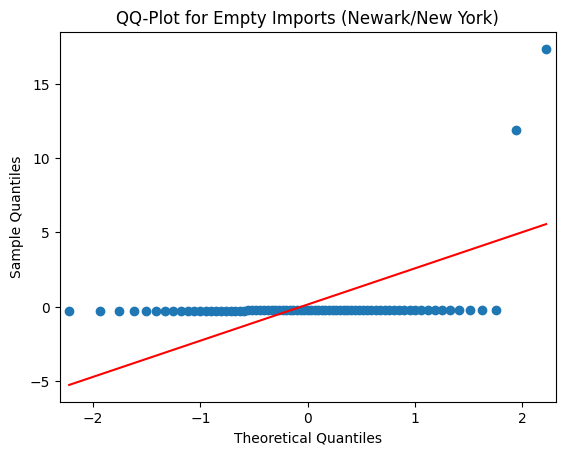
\includegraphics[width=0.7\textwidth]{qqplots_1.png}
		\end{figure}
	
		\begin{figure}[H]
			\caption{\label{qqplots_2} QQ-Plot para el total de importaciones (Newark/Nueva York)}
			\centering
			\hspace*{1cm}
			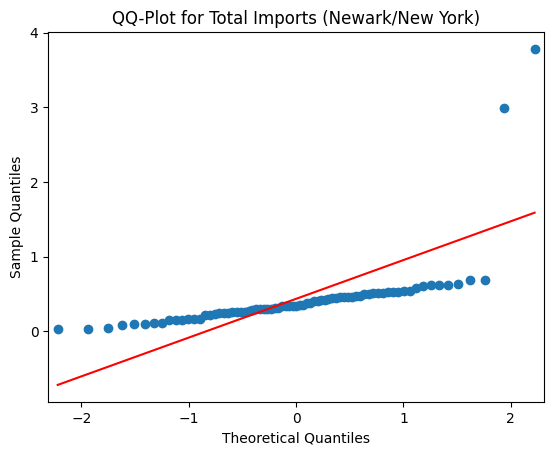
\includegraphics[width=0.7\textwidth]{qqplots_2.png}
		\end{figure}
	
		Para hacerse una idea de lo que representan los QQ-Plots anteriores, se deja un ejemplo para la variable "Total TEUs" o total de contenedores tratados por el puerto de Newark, en este caso. La figura (\ref{qqplots_3}) es útil para comparar como afectan los datos que se pueden considerar como outliers. Por ejemplo, hay un dato en la cola que se desvía un poco de la línea de tendencia. Pero en este caso no se considera un valor a tener en cuenta a la hora de realizar un filtrado de los datos. A diferencia de lo visto anteriormente.
		
		\begin{figure}[H]
			\caption{\label{qqplots_3} QQ-Plot para Total TEUs (Newark/Nueva York)}
			\centering
			\hspace*{1cm}
			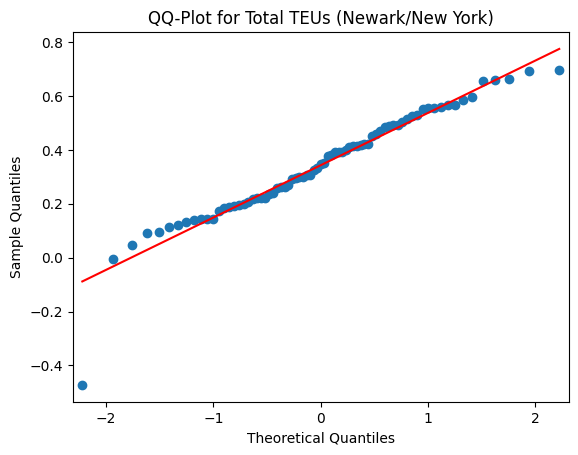
\includegraphics[width=0.7\textwidth]{qqplots_3.png}
		\end{figure}
	
		Como se observa en las figuras \ref{qqplots_1} y \ref{qqplots_2}, cada distribución tienen dos datos que se alejan mucho del resto. La pregunta que se plantea es si estos dos datos son los mismos y si afectan de la misma manera a distintas variables (especialmente para aquellas que puedan considerarse como "target").
		
		Para lo mencionado en el anterior párrafo, se enfrentó la variable 'Total Imports' (Ver su distribución en forma de histograma en \ref{hist_6}) frente a las distintas variables relacionadas con las drogas (Ver figura \ref{outliers_1}). 
		
		\begin{figure}[H]
			\caption{\label{hist_6} }
			\centering
			\hspace*{1cm}
			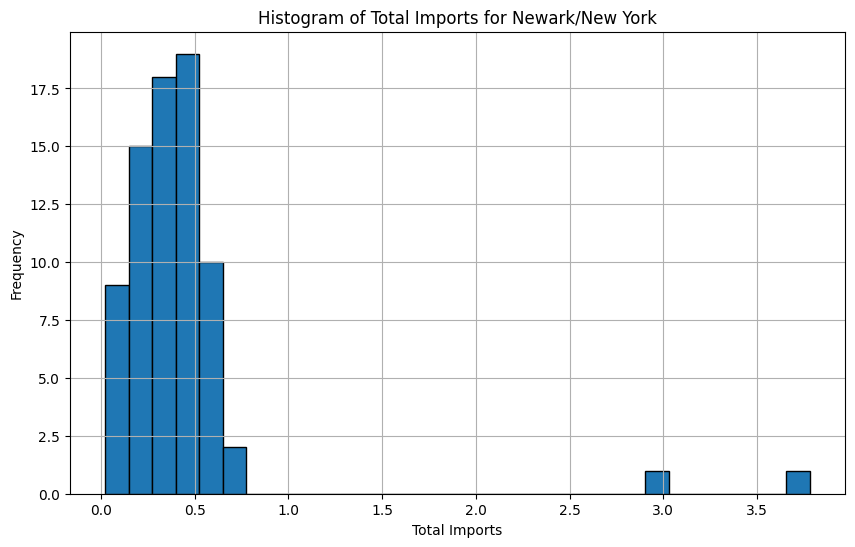
\includegraphics[width=0.7\textwidth]{hist_6.png}
		\end{figure}
		
		
		
		\begin{figure}[H]
			\caption{\label{outliers_1} }
			\centering
			\hspace*{1cm}
			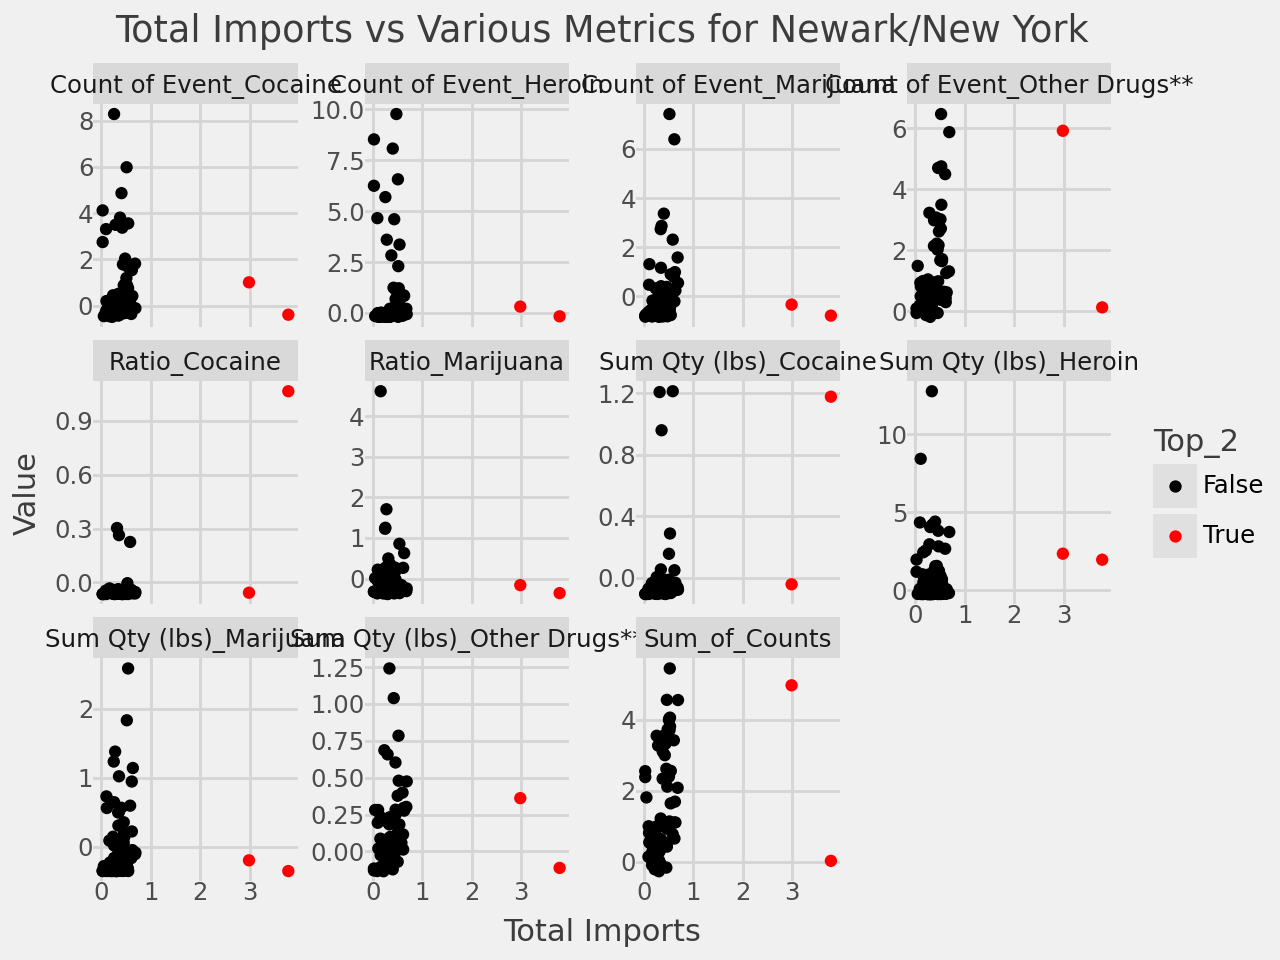
\includegraphics[width=\textwidth]{outliers_1.png}
		\end{figure}
	
		Esto sirve para asegurarse de que los dos outliers originales están alejados de todas las distribuciones. Como apunte, solo se muestra una serie de variables y se confirma que para el resto de variables se mantiene este comportamiento con esos datos alejados del resto. Conocer estas distribuciones sirve para facilitar la exclusión de las observaciones para estos outliers. Antes de aplicar el proceso de filtrado, comentar que también se ha tenido en cuenta el valor en el eje vertical de estos dos datos respecto de las distintas variables objetivo potenciales. Queda claro, entonces, de que son datos que van a aportar ruido sin importar la otra variable del par.
		
		Tras aplicar el siguiente fragmento de código:
		
		\begin{verbatim}
			# Filter the dataframe for 'Newark/New York'
			newark_data = filtered_data[filtered_data['Hub Portuario_name'] == 'Newark/New York']
			
			# Drop out values greater than 10 for columns with numeric data types
			ny_import_sorted['Top_2'] = ny_import_sorted['Total Imports'].rank(method='first', 
			ascending=False) <= 2
			numeric_columns = newark_data.select_dtypes(include='number').columns
			newark_data_filtered = newark_data[ny_import_sorted['Top_2'] == False]
		\end{verbatim}
	
		Tras aplicar el filtro definido en el fragmento de código anteior, se eliminan del conjunto de datos aquellos que estaban marcados en rojo en la figura \ref{outliers_1}.
		
		Por su parte, en las figuras \ref{qqplots_4} y \ref{qqplots_5} se muestra como quedaron las distribuciones QQ-Plots en 'Empty Imports' y 'Total Imports' y en \ref{outliers_2} su relación con las variables de drogas.
		
		\begin{figure}[H]
			\caption{\label{qqplots_4} QQ-Plot para Total TEUs (Newark/Nueva York)}
			\centering
			\hspace*{1cm}
			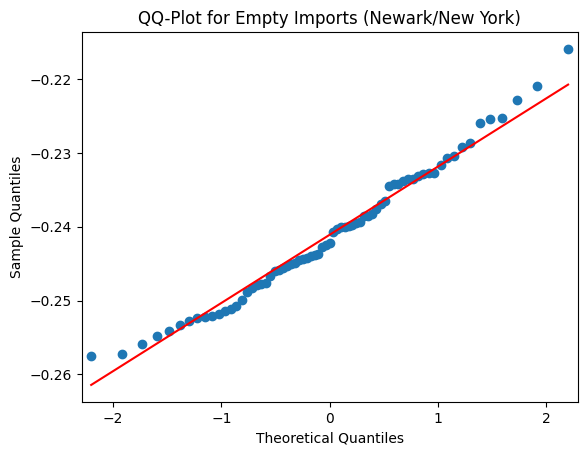
\includegraphics[width=0.8\textwidth]{qqplots_4.png}
		\end{figure}
	
		\begin{figure}[H]
			\caption{\label{qqplots_5} QQ-Plot para Total TEUs (Newark/Nueva York)}
			\centering
			\hspace*{1cm}
			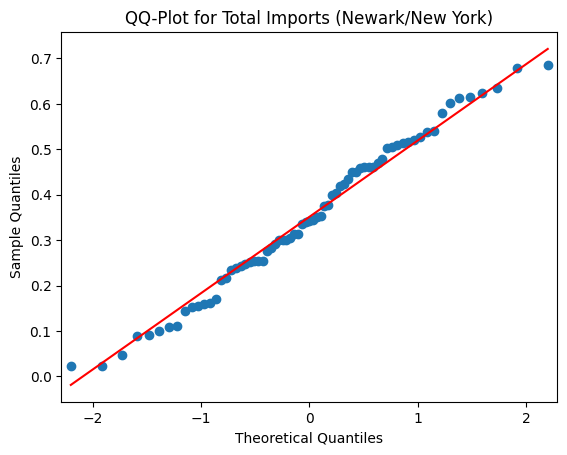
\includegraphics[width=0.8\textwidth]{qqplots_5.png}
		\end{figure}
	
		\begin{figure}[H]
			\caption{\label{outliers_2} }
			\centering
			\hspace*{1cm}
			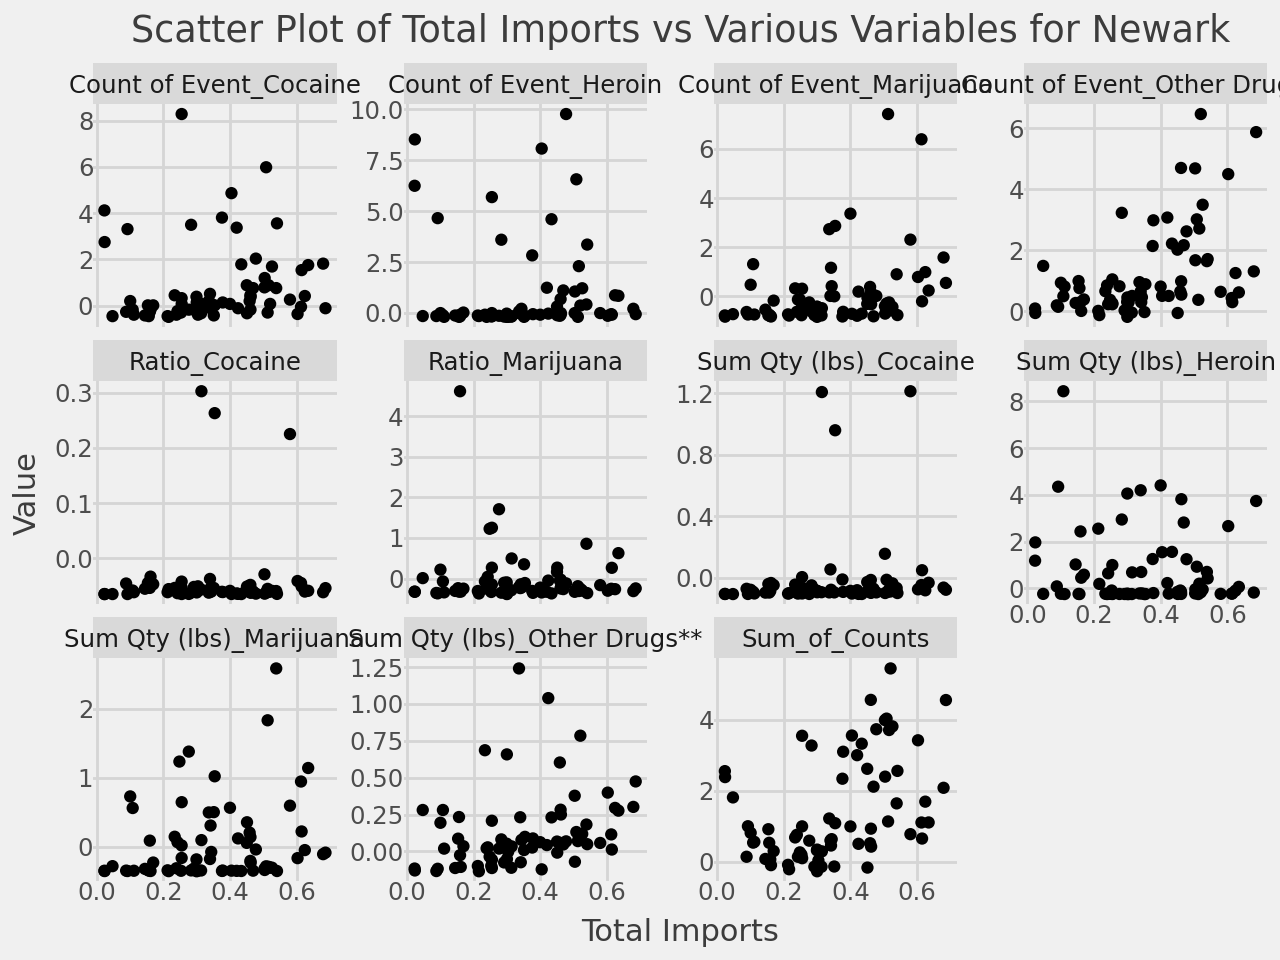
\includegraphics[width=\textwidth]{outliers_2.png}
		\end{figure}
	
		%Revisar esto
		\underline{Aplicando la transformación logarítmica}:\\
		Tras analizar los datos correspondientes al puerto de Newark en \ref{outliers_2}, se ha identificado un patrón particular en la variable Sum of Counts (último gráfico de dispersión).
		A priori, su distribución sugieren un comportamiento interesante para la construcción de modelos de predicción, lo que la convierte en una variable relevante a considerar.
		
		Sin embargo, al examinar su distribución en detalle -especialmente en comparación con otros hubs portuarios mediante el gráfico de boxplot en \ref{boxplot_5}- se evidencia una marcada asimetría con una cola pesada (\ref{hist_7}). Dada esta característica, se considera necesario aplicar una transformación logarítmica sobre los datos brutos para suavizar la distribución y aproximarlos a una distribución más próxima a la normal. Esta transformación deberá facilitar la modelización y mejorar la interpretación de resultados.
		
		\begin{figure}[H]
			\caption{\label{boxplot_5} Boxplot para hallar outliers en Sum of Counts}
			\centering
			\hspace*{1cm}
			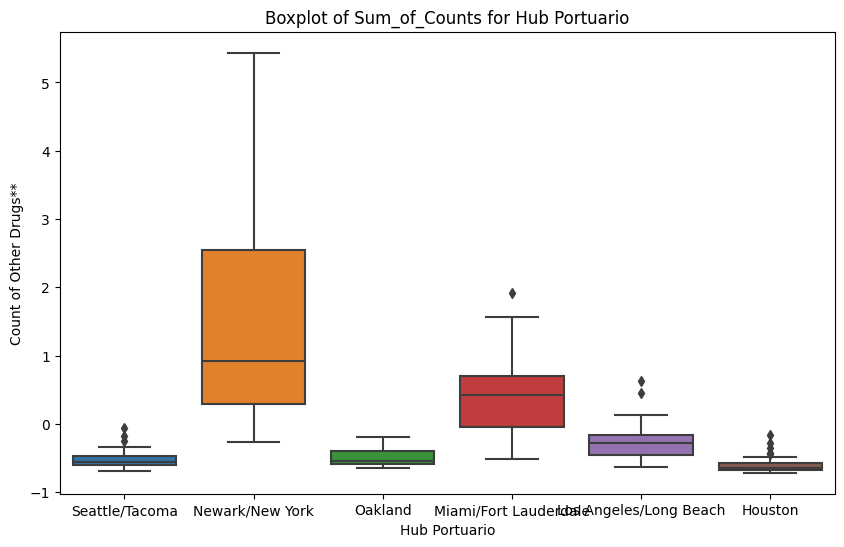
\includegraphics[width=0.9\textwidth]{boxplot_5.png}
		\end{figure}
		
		\begin{figure}[H]
			\caption{\label{hist_7} }
			\centering
			\hspace*{1cm}
			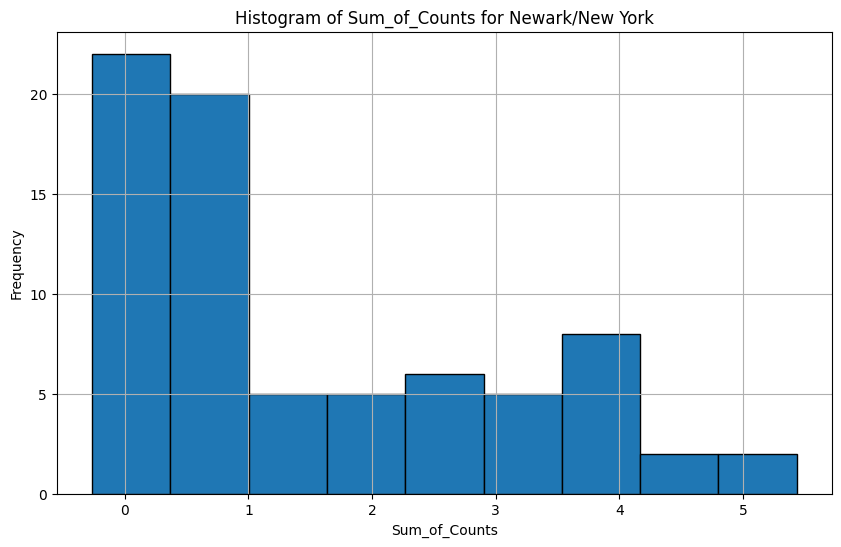
\includegraphics[width=0.9\textwidth]{hist_7.png}
		\end{figure}
		
		En la figura \ref{boxplot_5} se observa un pequeño error de asignación de etiquetas al eje vertical. En este caso no se trata de comparación respecto a la variable "Count of  Other Drugs**" sino de "Sum of Counts".
		
		% Definir proceso aqui
		
		
		\begin{figure}[H]
			\caption{\label{boxplot_6} Boxplot para Sum of Counts}
			\centering
			\hspace*{1cm}
			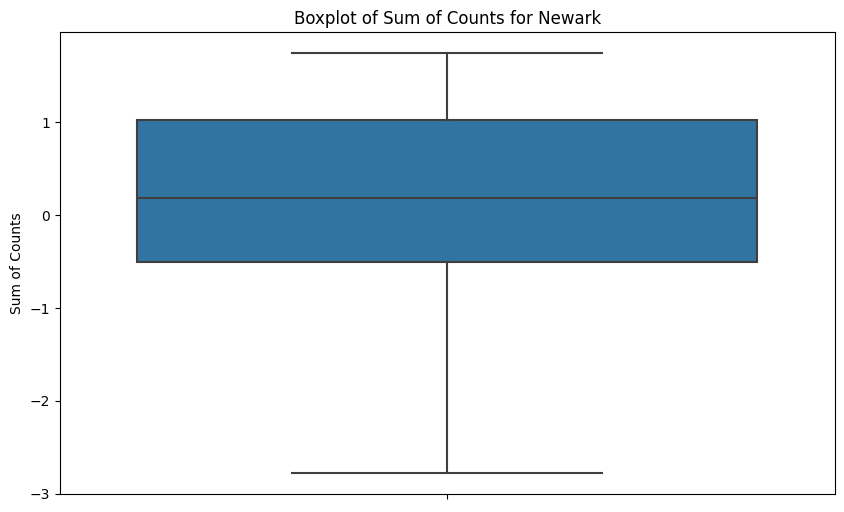
\includegraphics[width=0.8\textwidth]{boxplot_6.png}
		\end{figure}
		
		\begin{figure}[H]
			\caption{\label{hist_8} }
			\centering
			\hspace*{1cm}
			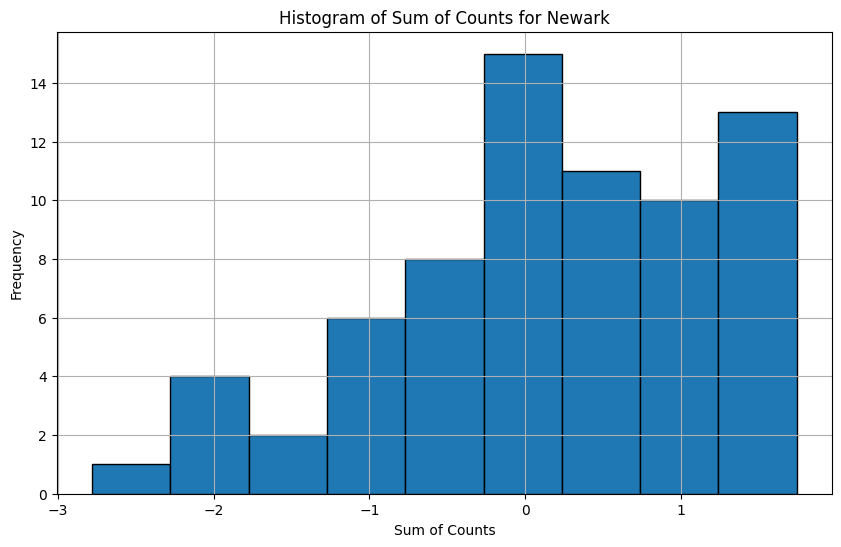
\includegraphics[width=0.8\textwidth]{hist_8.png}
		\end{figure}
		
		Los hallazgos obtenidos a partir de esta transformación abren la posibilidad de desarrollar un modelo predictivo para intentar estimar el número de incautaciones exitosas en el puerto de Newark.
		
		Tras la aplicación de la transformación logarítmica y la estandarización para los datos del puerto de Newark, el gráfico de dispersión para las variables 'Sum of Counts' y 'Total Imports' queda tal y como se muestra en la figura \ref{}
		
		\begin{figure}[H]
			\caption{\label{scattered_2} Gráfico de dispersión Importaciones y Redadas en Newark tras transformación logarítmica y estandarización }
			\centering
			\hspace*{1cm}
			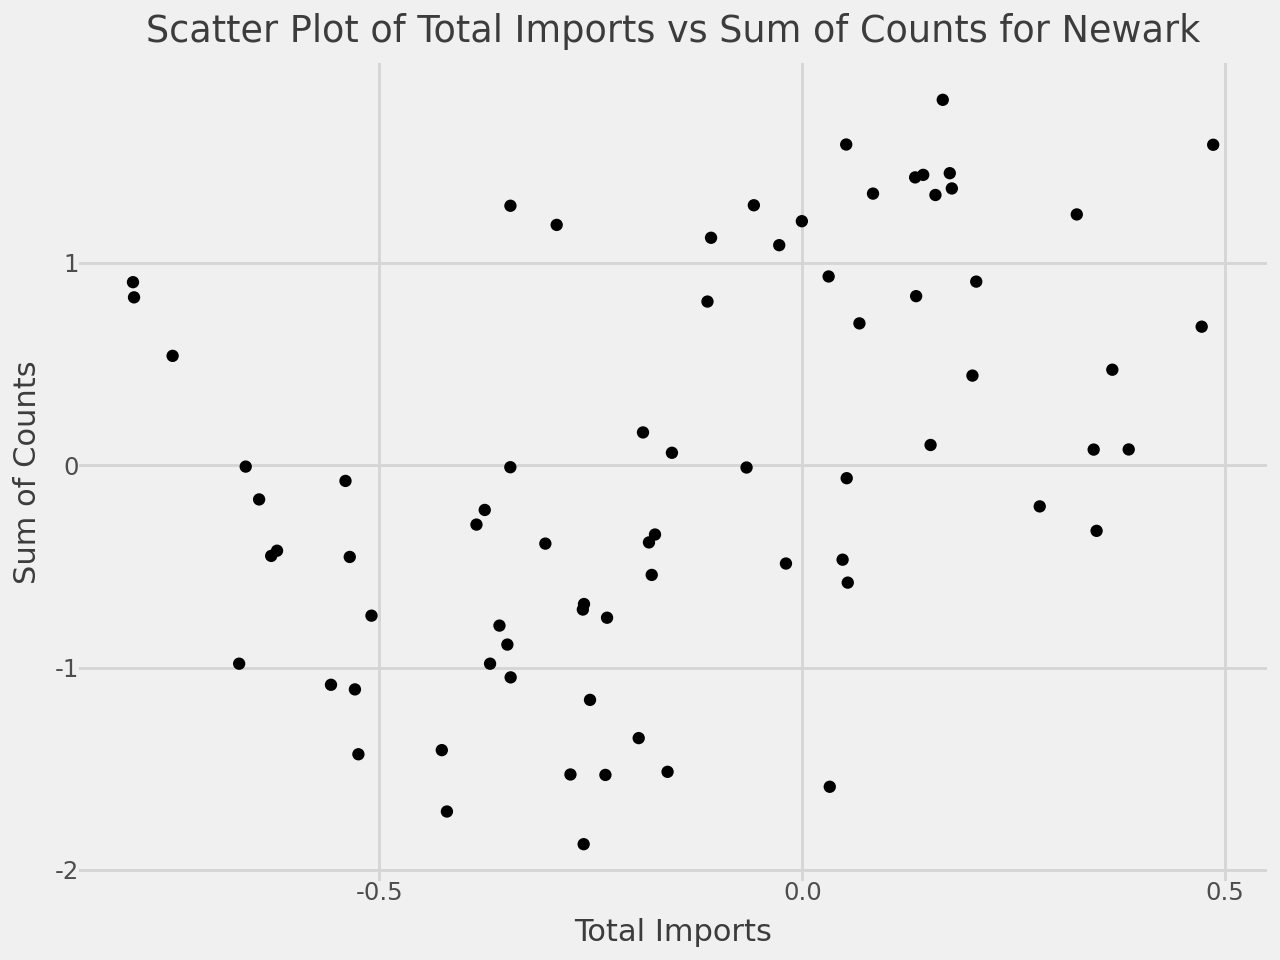
\includegraphics[width=0.7\textwidth]{scattered_2.png}
		\end{figure}
	
		Como comentario debido a la limpieza de outliers en este caso, se logró una representación de los datos con mayor nivel de detalle. Por otra parte, la matriz de correlación resultante tras aplicar la transformación logarítmica y posterior estandarización varió respecto a la matriz original. El resultado quedó como se muestra en la figura \ref{matrix_corr_7}
		
		\begin{figure}[H]
			\caption{\label{matrix_corr_7} Matriz de correlaciones tras transformación logaritmica y estandarizacion}
			\centering
			\hspace*{1cm}
			\includegraphics[width=0.7\textwidth]{matrix_corr_7.png}
		\end{figure}
	
	\subsection{\label{split}Estrategia de división de datos}
	% Train-Test Split, Validación Cruzada, GridSearch para estimación de hiperparámetros.
	Para garantizar la correcta evaluación del rendimiento de los modelos desarrollados en este trabajo, resultó esencial definir una estrategia de división de datos. Con independencia del tipo de problema que se abordase, se consideró dejar como conjunto de datos libres de ser entrenados a todos aquellos con fechas más recientes a su captura (siendo la mayoría de ellos pertenecientes al año 2024). También se aprovechó esta circunstancia debido a la falta de claridad sobre el modelo a elegir para responder al problema y se consideró viable reciclar esta división entre conjuntos de entrenamiento y de test ante la incertidumbre.
	
	El resto de datos fueron usados para entrenar los distintos modelos junto con la evaluación y optimización de hiperparámetros para mejorar la precisión del modelo. La librería scikit-learn (\cite{scikit-learn}) permite realizar tanto la división del conjunto de datos con train test split como la estimación de los hiperparámetros con GridSearchCV, entre otros.
	
	A continuación un ejemplo de partición del conjunto de datos de entrenamiento y test para el caso del puerto de Fort Lauderdale (Port Everglades)
	\begin{verbatim}
		# Use last year for test
		# Convert 'Date' to datetime
		everglades_data_input['Date'] = pd.to_datetime(everglades_data_input['Date'])
		
		# Split the data
		train_data = everglades_data_input[everglades_data_input['Date'] < '2024-01-01']
		test_data = everglades_data_input[everglades_data_input['Date'] >= '2024-01-01']
	\end{verbatim}

	En lugar de realizar una partición aleatoria, se decidió forzar a dejar los datos del último año como test. Esto se debe a que originalmente, como se ha ido exponiendo a lo largo del trabajo, no había una finalidad u objetivo concreto. Y como no estaba concreto hacia donde se quería orientar el modelo, se mantuvo abiertas las posibilidades de realizar modelos de series temporales, así como de otras predicciones en forma de regresión.
	
	Teniendo en cuenta que se tenían 75 meses de partida y en el mejor de los casos, se reservarían los doce últimos para el conjunto de test, el ratio del split vendría a ser: 84\% de los datos para entrenamiento, frente al 16\% para evaluar como generaliza el modelo.
	
	% Representacion gráfica con una barra que distinga train de test.

\newpage
\section{\label{Diseño}Diseño del Modelo}
En esta sección se muestran los algoritmos y técnicas que se han utilizado para intentar llevar a buen puerto el estudio en este proyecto. El objetivo de este trabajo se centra en intentar averiguar tendencias o patrones que relacionen el volumen de cargamento movido en contenedores gestionados por puertos con la cantidad de droga incautada. Así como para algún caso concreto, intentar hallar la relación temporal entre los mismos.

	\subsection{Algoritmos y técnicas de Machine Learning utilizados}

	% Hiperparámetros y técnicas de optimización.
	
	Como se vio en la sección \ref{motivacion}, hubo ciertas dificultades a la hora de plantear el target y, en definitiva, lo que quiere predecir el modelo. Se han desarrollado dos pequeños modelos al respecto: uno para predecir la cantidad incautada por redada en Newark (Estados de Nueva Jersey y Nueva York) y otro sobre la cantidad de redadas con éxito(*) en Port Everglades (Área Metropolitana Miami-Fort Lauderdale).
	
	\subsubsection{Implementación del algoritmo de clustering para detectar hubs portuarios}
	Esta subsección es más bien un pequeño recordatorio de lo que se desarrolló en \ref{clustering}.
	
	Dada la gran cantidad de puertos obtenidos desde las fuentes originales estaba muy desbalanceada con el pequeño número de oficinas del CBP de Estados Unidos, se tomó la decisión de reagrupar aquellos puertos que estuviesen geográficamente próximos. Para ello, se decidió realizar una sencilla y rápida implementación del algoritmo K-Means para las latitudes y longitudes de los barcos detectados en las costas de Estados Unidos que reportaran un status con 'movilidad reducida' o 'atracados' (desde luego, sin rumbo con motor). De ahí, tal y como se mencionó en \ref{clustering}, se generaron 30 clusters originales, equivalentes a 30 hubs portuarios. Sin embargo, dadas las complicaciones a la hora de generalizar los datos, en un primer momento se decidió extraer un único hub portuario (y, en el momento que ocupa el desarrollo de este trabajo, expandirlo a media docena que tuvieran una asignación clara con su CBP). A continuación se deja constancia de la implementación del algoritmo K-Means original para tratar de hallar hubs portuarios importantes.
	
	\begin{verbatim}
		from sklearn.metrics import silhouette_score
		
		silhouette_scores = []
		k_range = range(2, 32) 
		
		for k in k_range:
		kmeans = KMeans(n_clusters=k, random_state=42, n_init=10)
		labels = kmeans.fit_predict(coord_cargos_in_port_df)
		silhouette_scores.append(silhouette_score(coord_cargos_in_port_df, labels))
		
		optimal_k = k_range[np.argmax(silhouette_scores)]  # K = 31
		
		# Run KMeans clustering
		kmeans = KMeans(n_clusters=optimal_k, random_state=42, n_init=10)
		kmeans.fit(coord_cargos_in_port_df)
	\end{verbatim}

	En la sección de Anexos se pueden ver las asignaciones de cada cluster a cada hub portuario (latitud y longitud)
	
	
	Recuérdese que las imágenes del resultado se pueden ver en la figura \ref{map_cluster_3} de la sección \ref{data origin})
	
	
	\subsubsection{\label{stProphet}Implementación del algoritmo de Prophet para el análisis de series temporales}
	Algunos de los motivos que me llevó a plantear un modelo que ajustase series temporales fueron los resultados arrojados para incautaciones de drogas en el puerto de Fort Lauderdale. A continuación se muestran tres casos en los que se comparan las tendencias de importaciones (de contenedores con cargamento) junto con redadas de cocaína, marihuana y otras drogas. En la imagen \ref{miami_ts_1} que la distribución de los datos está ajustada a un escalado min-max (entre 0 y 1.00) y en las tendencias que tienen. Esto último abrió la posibilidad de orientar el trabajo a una aproximación de tendencias (derivadas de funciones suavizadas con filtros de bajas frecuencias) \ref{trabajo futuro}.
	
	\begin{figure}[H]
		\caption{\label{miami_ts_1} Serie Temporal en Puerto Fort Lauderdale con redadas de cocaína}
		\centering
		\hspace*{1cm}
		\includegraphics[width=0.8\textwidth]{miami_ts_1.png}
	\end{figure}

	Aunque originalmente una de las principales motivaciones para realizar el trabajo era predecir la incautación de droga en base a las entradas de cargamento (importaciones) en el puerto, al final se acabaron dejando estos modelos a modo de experimentación. A simple vista de la imagen dada, aunque más clara para el caso de evaluar las redadas de otras drogas (ver la figura \ref{miami_ts_2}), se ven tramos en los que coinciden la tendencia y la proporción en la subida (o bajada) para las series temporales que se comparan. Si bien es cierto que la variable de "loaded imports" tiene cambios de tendencia donde no las tiene "other drugs".
	
	\begin{figure}[H]
		\caption{\label{miami_ts_2} Serie Temporal en Puerto Fort Lauderdale con redadas de otras drogas}
		\centering
		\hspace*{1cm}
		\includegraphics[width=0.7\textwidth]{miami_ts_2.png}
	\end{figure}

	Se podría realizar una transformación de los datos para "Count of Event Other drugs**" (línea roja en \ref{miami_ts_2}) de la forma:
	%
	$$F(x) = |f(x) - g(x)| + g(x)$$
	%
	para que tenga una línea de tendencia parecida a "Loaded Imports".
	
	Para la pequeña implementación de un modelo de series temporales en prophet se ha usado "Count of Event Other drugs**" como variable objetivo y "Loaded Imports" como regresor exógeno.
	
	A continuación se deja un pequeño fragmento de código para la llamada al constructor de prophet, ajuste y predicción:
	\begin{verbatim}
		m = Prophet()
		m.add_regressor('Loaded Imports')
		m.fit(df_imports_train)
		
		# Make future dataframe for prediction
		future = m.make_future_dataframe(periods=len(df_imports_test))
		# Add the regressor values for both training and prediction periods
		future['Loaded Imports'] = pd.concat([df_imports_train['Loaded Imports'], df_imports_test['Loaded Imports']])
		
		# Make predictions
		forecast = m.predict(future)
	\end{verbatim}

	También en las secciones \ref{interpretacion} y \ref{trabajo futuro} se comentan los cambios de tendencia. Especialmente en el caso de \ref{miami_ts_2}, o por qué en la figura \ref{miami_ts_3} hay un lag entre las redadas de marihuana y el cargamento importado.
	
	\begin{figure}[H]
		\caption{\label{miami_ts_3} Serie Temporal en Puerto Fort Lauderdale con redadas de Marihuana}
		\centering
		\hspace*{1cm}
		\includegraphics[width=0.8\textwidth]{miami_ts_3.png}
	\end{figure}
	
	% Implementacion del modelo de serie temporal para Miami
	También, como complemento a los modelos de series temporales a prophet, se implementó un pequeño modelo sarimax incluido en la librería statsmodel y un XGBoost.
	
	\subsubsection{\label{hiperCV}Implementación de la matriz de ajuste hiperparámetros para los distintos algoritmos de regresión}
	% Copiar código de GridSearchCV
	Tras explorar, revisar y manipular los datos brutos, una de las aproximaciones que se valoró fue la referente a tratar de modelar el problema como un problema de regresión. Casos como el de la relación entre variables 'Sum of Counts' con 'Total Imports' para el puerto de Newark/Nueva York daban lugar a pensar en ello. Dado que la librería scikit-learn ofrece muchas posibilidades en lo que a algoritmos para resolver problemas de regresión, se decidió crear un pool de regresores de distinta índole (lineal, AdaBoost, Árboles de decisión...) para compararlos entre ellos. Como apunte, se acotó el problema a algoritmos definidos en scikit-learn (dejando fuera de aquí, en este caso, otros de interés como, por ejemplo, XGBoost). A continuación se muestran todos los regresores (con sus distintas combinaciones de hiperparámetros) que se estimaron oportunos para intentar predecir la relación de las variables mencionadas un poco más arriba.
	
	\begin{verbatim}
		regressors = {
			'LR': LinearRegression(),
			'adaBoostRegressor': AdaBoostRegressor(random_state=256),
			'baggingRegressor': BaggingRegressor(random_state=256),
			'GBR': GradientBoostingRegressor(random_state=256),
			'DT': DecisionTreeRegressor(random_state=256)
		}
	\end{verbatim}

	Para forzar al modelo a escoger los mejores hiperparámetros, se hizo uso de las funciones de validación cruzada para búsqueda y validación de los mismos:
	
	\begin{verbatim}
		regressorsCV = GridSearchCV(
		estimator=regressor,
		param_grid=params,
		scoring='r2',
		cv=5
		)
		regressorsCV.fit(X_train, y_train)
	\end{verbatim}

	Se estimaron diversas métricas de estimación del error de predicción (MAE, MedAE, MAPE, etc.), siendo R² la más sencilla de interpretar sobre la calidad del modelo. En la subsección \ref{eval performance} se verá que, a pesar de todo, al modelo le cuesta predecir.
	
	Comparando los desempeños entre los distintos modelos se puede concretar cuál de ellos es mejor o, simplemente, hacerse una idea con los datos de entrenamiento.
	
	\subsection{\label{implementacionPractica}Implementación Práctica del Modelo}
 	% Descripción de las tareas realizadas para implementar el proyecto.
 	% Se destacan las principales actividades y decisiones.
 	% Fases de desarrollo del proyecto.
 	En este apartado, se describen las tareas realizadas para llevar a cabo el proyecto. Dado la dificultad para encontrar un objetivo concreto lo suficientemente atractivo para las condiciones de los datos recopilados, se dejó la puerta abierta a intentar aproximar el modelo para distintos casos: una aproximación de un modelo de regresión a partir de los datos curados del puerto de Nueva York (Newark, \ref{NY model}) e inclusión una predicción para un modelo de series temporales del puerto de Miami (Fort Lauderdale, \ref{FL model}).
 	
 	\subsubsection{\label{NY model} Modelo para el puerto de Nueva York}
 	Para el caso del modelo del puerto de Newark, se generó un diccionario de regresores (mencionados en la sección \ref{hiperCV}) para intentar predecir la variable "Sum of Counts" a partir de: Loaded Exports, Empty Imports, Loaded Imports, Total TEUs y Total Imports. El criterio de elegir estas variables predictoras se basó en los resultados de la matriz de correlaciones de la figura \ref{matrix_corr_7}.
 	
 	Por su parte, estos regresores fueron evaluados tanto con la métrica de R² como de MAPE tal y como están definidas en la API de scikit-learn.
 	
 	Junto a esto, tal y como se mencionó en \ref{split}, para el conjunto de datos de entrenamiento se dejaron todos los datos excepto los del 2024 (lo que supuso un 84\% sobre el total) y los correspondientes al 2024 (16\% restante) como conjunto de test.
 	
 	\begin{verbatim}
 		test_scores = []
 		
 		for name in list(params.keys()):
 		print(name)
 		print("Numero de configuraciones: ", pd.DataFrame.from_dict(regressorsCV[name].cv_results_).shape[0])
 		
 		# Get sorted results, ensuring lower MAPE is better
 		aux = pd.DataFrame.from_dict(regressorsCV[name].cv_results_).sort_values(by="mean_test_score", ascending=True).iloc[0]
 		
 		# Ensure MAPE is positive
 		mape_cv_test = abs(aux['mean_test_score'])
 		mape_cv_train = abs(aux['mean_train_score'])
 		
 		# Get best model and compute MAPE
 		best_model = regressorsCV[name].best_estimator_
 		mape_train = mean_absolute_percentage_error(y_train, best_model.predict(X_train))
 		mape_test = mean_absolute_percentage_error(y_test, best_model.predict(X_test))
 		
 		test_scores.append((name, mape_train, mape_cv_train, mape_cv_test, mape_test))
 	\end{verbatim}
 	El fragmento de código anterior tiene su equivalente para evaluar modelos usando la métrica de R². Los resultados arrojados se muestran en la sección \ref{eval performance}.
 	
 	
 	\subsubsection{\label{FL model} Modelo para el puerto de Fort Lauderdale}
 	
 	% 
 	Por su parte, tal y como se expuso en la subsección \ref{stProphet} también se probó un modelo de series temporales con la librería prophet para predecir las incautaciones en Fort Lauderdale.
 	
 	En este caso, incluso se ha generado una matriz (grid) de hiperparámetros para intentar escoger el mejor modelo de regresión de series temporales. En este caso se ha buscado incluir puntos de cambio de tendencia (changepoints) en los hiperparámetros a ajustar.
 	Se deja el código a disposición en la sección de anexos.
 	
 	La combinación de hiperparámetros para el modelo de Prophet que ajusta unos valores de una forma superior al resto de combinaciones de hiperparámetros es:
 	
 	\begin{verbatim}
 		m = Prophet(
 		changepoint_prior_scale=0.01,  # Controls flexibility (default is 0.05)
 		changepoint_range=0.8,        # Where changepoints can occur (default is 0.8)
 		n_changepoints=30             # Number of potential changepoints (default is 25)
 		)
 	\end{verbatim}
 
 	Como se mencionó en \ref{stProphet}, también se generaron modelos con las librerías statsmodel y xgboost. En el caso del primero, se generó un modelo sarimax. En todos los casos, se incluyó "Loaded Imports" como regresor exógeno.
 	
 	Aquí se deja un pequeño fragmento de código con XGBoost:
 	\begin{verbatim}
 		import xgboost as xgb
 		df_xgb.rename(columns={'Date': 'ds', 'Ratio_Other Drugs**': 'y', 
 			'Loaded Imports': 'loaded_imports'}, inplace=True)
 		
 		# Convertir la columna de fecha a datetime
 		df_xgb['ds'] = pd.to_datetime(df_xgb['ds'])
 		
 		# Dividir en conjunto de entrenamiento y prueba según la regla dada
 		df_train = df_xgb[df_xgb['ds'] < '2024-01-01']
 		df_test = df_xgb[df_xgb['ds'] >= '2024-01-01']
 		
 		[...]
 		
 		# Crear y entrenar el modelo XGBoost
 		xgb_model = xgb.XGBRegressor(objective='reg:squarederror', n_estimators=100, learning_rate=0.1, max_depth=3)
 		xgb_model.fit(X_train, y_train)
 		
 		# Realizar predicciones en test
 		y_pred_xgb = xgb_model.predict(X_test)
 	\end{verbatim}
 
 	En la siguiente sección se muestran las evaluaciones del desempeño para cada modelo. Y va a servir para responder en parte a la pregunta que dio origen a este problema: ¿se puede predecir la cantidad de droga incautada en una región a partir de la actividad comercial en un puerto marítimo?

	\subsection{\label{eval performance}Evaluación del rendimiento}
	% Métrica utilizadas.
	% Comparaciones con alternativas.
	En esta sección se evaluan los algoritmos aplicados a los distintos modelos. Por un lado, los distintos regresores para el caso del puerto de Newark (\ref{evalNewark}) y por el otro, el acercamiento a un análisis de series temporales simplificado para el puerto de Everglades en Fort Lauderdale (\ref{evalFL}).
	
	\subsubsection{\label{evalNewark} Caso puerto de Newark}
	Para este primer caso, se han entrenado y comparado una regresión lineal, un árbol de decisión, un regresor con Bagging, un AdaBoost Regressor y Gradient Boost Regressor. Como se expuso en \ref{hiperCV} se reentrenaron los modelos para un pool de hiperparámetros mediante GridSearchCV.
	
	Las métricas utilizadas para evaluar los algoritmos han sido: MAPE (Mean Average Percentual Error) y R². A continuación se muestran los resultados con respecto a las dos métricas:
	
	\begingroup
	\begin{table}[H]
	\caption{\label{tabla}}
		\centering
		\setlength{\tabcolsep}{3pt}
		\renewcommand{\arraystretch}{1.5}
%		\setlength{\abovesep}{10pt}
		\begin{tabular}{|c|c|c|c|c|c|c|}
			\hline
			Regressor & mape\_train & mape\_cv\_train & mape\_validation & mape\_test \\
			\hline
			Linear Regression & 2.121 & 1.8821 & 4.7155 & 3.210 \\
			AdaBoost Regressor & 1.3500 & 10.7106 & 11.3422 & 10.5980 \\
			Bagging Regressor & 1.8094 & 4.6164 & 5.8572 & 4.1661 \\
			Gradient Boost Regressor & 1.5098 & 3.1376 & 4.1490 & 1.8605 \\
			Decision Tree Regressor & 1.1907 & 2.8116 & 5.3514 & 12.7950 \\
			\hline
		\end{tabular}
	\end{table}
	\endgroup
	
	\begingroup
	\begin{table}[H]
		\caption{\label{tabla}}
		\centering
		\setlength{\tabcolsep}{3pt}
		\renewcommand{\arraystretch}{1.5}
		%		\setlength{\abovesep}{10pt}
		\begin{tabular}{|c|c|c|c|c|c|c|}
			\hline
			Regressor & r2\_train & r2\_cv\_train & r2\_validation & r2\_test \\
			\hline
			Linear Regression & 0.4384 & 0.4635 & -11.4976 & -0.9048 \\
			AdaBoost Regressor & -0.7262 & -3.1662 & -58.4642 & -5.6579 \\
			Bagging Regressor & 0.8465 & 0.6500 & -15.2525 & -2.0731 \\
			Gradient Boost Regressor & 0.7463 & -8.2508 & -7.3105 & -1.5215 \\
			Decision Tree Regressor & 0.6910 & 0.8401 & -7.9630 & -2.6052 \\
			\hline
		\end{tabular}
	\end{table}
	\endgroup
	
	Como se expondrá en el capítulo de "Interpretación de resultados" (\ref{interpretacion}), los resultados arrojados muestran que ninguno de los modelos planteados, para los hiperparámetros optimizados, genera un modelo de calidad.

	Esto implica que el problema no esté en los algoritmos, ni siquiera tanto en su configuración de hiperparámetros sino en un error de concepción del problema para los datos disponibles.
	
	\subsubsection{\label{evalFL} Caso puerto de Everglades - Fort Lauderdale}
	% Series temporales
	Modelo muy simple para realizar una regresión de series temporales. Se han excluido periodos estacionales, cambios de tendencia... Se ha mantenido exclusivamente la tendencia a largo plazo. Debido a esto, los resultados del ajuste son bastante pobres.
	
	\underline{Resultados en Test}: \\
	\begin{itemize}
		\item[-] R²: -9.1261 (los datos del ajuste del modelo son más grandes, y por lo tanto, peores que si usasemos la media).
		\item[-] MAPE: 382,9\%
	\end{itemize}

	\underline{Resultados en Train}: \\
	\begin{itemize}
		\item[-] MAPE: 12,41\%
	\end{itemize}
	
	

\newpage
\section{\label{interpretacion}Interpretación de los resultados}
Ninguno de los modelos fue capaz de predecir el comportamiento a futuro para el puerto de Newark. El caso para el puerto de Fort Lauderdale se cuenta como más experimental respecto al uso de la librería. En ningún caso puede considerarse los resultados como válidos para aceptar ninguno de los modelos. Esto hace pensar que el problema de base esté en la concepción del problema.

	\subsection{Visualización de resultados}
	
	% Incluir gráficos para modelo de regresores
	En esta subsección se dejan algunas gráficas con los resultados de los ajustes (para el modelo de series temporales):
	
	\begin{figure}[H]
		\caption{\label{st_test_1} Serie temporal con Prophet para tendencia de incautaciones en Fort Lauderdale}
		\centering
		\hspace*{1cm}
		\includegraphics[width=\textwidth]{st_test_1.png}
	\end{figure}

	\begin{figure}[H]
		\caption{\label{st_test_2} Zoom para datos de test (2024) para Fort Lauderdale}
		\centering
		\hspace*{1cm}
		\includegraphics[width=0.6\textwidth]{st_test_2.png}
	\end{figure}

	La figura \ref{st_test_1} representa el ajuste simplificado mediante las funciones de la librería prophet para la serie de datos ordenados cronológicamente para estimar la incautación de droga mensual en el puerto de Fort Lauderdale. Se ha incluido la variable "Loaded Imports" como regresor exógeno. Como se puede apreciar en la imagen, el modelo está tan simplificado (y automatizado) que no se ha concretado ninguna periodicidad (funciones de autocorrelación, aplicaciones de lags o retardos, etc.). La figura \ref{st_test_2} es un zoom de los datos de test (predicciones para 2024).
	
	
	\subsection{\label{sesgos}Sesgos y limitaciones}
	Para el caso de las predicciones usando regresores de distinta índole en el caso del puerto de Newark, se ve que ninguno de ellos ajusta correctamente. En prácticamente todos los modelos, el valor en test de R² es negativo, lo cual quiere decir que si se hubiese trazado la recta de la media de los valores, ésta última hubiera ajustado mejor que cualquiera de los modelos. Si observamos los datos en el conjunto de entrenamiento (datos que abarcan desde 2018 hasta 2023), en ningún caso se puede decir que el ajuste sea anómalamente alto. Esto no quiere decir que no haya overfitting (que lo hay), pero en ningún modelo en entrenamiento supera el R² = 0.85 (si acaso Gradient Boost Regressor). En cambio, los datos arrojados por los conjuntos de validación (media de resultados para una estratificación K-Fold igual a cinco) dan a entender la alta variabilidad entre los datos, lo cual dificulta mucho que el modelo aprenda por cada nuevo dato. Esto ha sido la tónica general a lo largo de este trabajo y que viene a resumir lo que desde las primeras páginas se barruntaba: con los datos en la mano, no se puede relacionar la actividad portuaria con la cantidad de droga incautada. Porque precisamente hay que distinguir entre "droga incautada" de droga que entra en un puerto. Si esa droga incautada representa un porcentaje muy pequeño respecto a la que, téoricamente, entra por el mismo, a menos que sea una muestra muy representativa, va a producir sesgos y distorsiones para cualquier modelo. No solo eso, es posible que haya terceros factores que influyan más en la relación entre actividad y droga incautada: política de lucha contra la droga, presupuestos, recursos humanos, demanda, consumo, competencia de otros territorios consumidores...
	
	Por su parte, para el caso de series temporales, el rango cronológico de datos parece insuficiente para tomar en consideración tendencias a largo plazo, encontrar patrones de estacionalidad, determinar cual es el nivel de variabilidad entre datos... 

\newpage
\section{\label{trabajo futuro}Conclusiones y trabajo futuro}
A lo largo de este trabajo se han seguido los pasos metodológicos correspondientes a un proyecto de ciencia de datos. Desde la captura e integración de los datos, su limpieza, procesado y curado hasta la generación de modelos de Machine Learning que intentasen predecir el comportamiento de las variables predictoras a una variable target. La decisión para elegir la variable target no fue sencilla en absoluto. Dada la disparidad de valores, de objetos de interés y de estudio, incluso se recurrió a técnicas de ingenería de características para generar potenciales variables target que pudiesen satisfacer la pregunta que se planteaba para desarrollar el modelo. Y es que, ante todo, el modelo intentó predecir la cantidad de droga incautada a partir de la actividad portuaria. En un primer momento, se intentó integrar todos los puertos en un mismo modelo, para más adelante realizar un modelo para cada puerto en particular.

En este trabajo, lo que se ha analizado ha sido la relación entre el tráfico de contenedores en los principales puertos de EE.UU. y la cantidad de droga incautada por las oficinas de campo del CBP. Como se comentó en \ref{sesgos}, la confusión entre droga incautada (datos tangibles y contabilizados) con droga entrante de forma clandestina (estimaciones y aproximaciones) ha sido principalmente el error de concepto que ha impedido generar modelos correctos. En parte por la falta de datos del lado de las variables predictoras (tanto observaciones como variables). Pocos datos, 75 meses, para un asunto que quizá requiera un rango mayor en este sentido, que pueda abarcar muchos más años. Pero sobre todo, pocas variables y muy rendundantes en muchos casos. Es decir, los datos del CBP limitan el rango temporal. Los datos de actividad portuaria limitan la calidad y variación de información para los predictores.

En esta sección se ponen evidencia hallazgos relevantes encontrados, la posible aplicabilidad del modelo entornos reales, las limitaciones del trabajo y líneas de investigación futuras.

Todos los programas, recursos, archivos, fuentes y datos están disponibles en la siguiente dirección:
\url{https://github.com/GonzaloLopezS/TFM_AFI_2025}

	\subsection{Hallazgos relevantes}
	A pesar de todo se han encontrado los siguientes hallazgos:
	\begin{itemize}
		\item [-] Se han identificado ciertos puertos con una mayor recurrencia de incautaciones en función del tipo de droga.
		\item [-] Dados los resultados de los modelos predictivos, se ha concluido que la actividad en un puerto no es suficiente para teorizar la cantidad incautada en la misma región.
		\item [-] Se ha realizado un análisis exploratorio de datos profundo que ha permitido detectar, en algunos casos, aparentes patrones temporales para la actividad portuaria y las incautaciones de droga.
	\end{itemize}
	
	\subsection{Aplicabilidad del modelo en entornos reales}
	La parte de análisis de datos puede ser de utilidad para agencias de seguridad y control aduanero. Especialmente para especializarse en la incautación y prevención de entrada de algún tipo de droga en concreto. Esto puede servir para:
	\begin{itemize}
		\item [-] Optimizar la asignación de recursos para inspecciones en puertos con mayor probabilidad de tráfico ilícito.
		\item [-] Integrar los datos obtenidos en bases de datos más actualizadas y con mayor rango temporal.
	\end{itemize}
	
	\subsection{Limitaciones del trabajo}
	A pesar de obtener algunos hallazgos, la tónica general del estudio viene precedida por una serie de limitaciones: tanto a nivel de concepción, de datos obtenidos como del modelo:
	
	\begin{itemize}
		\item [-] Pese a tratarse de datos de calidad certificada (datos oficiales validados), su limitación a nivel de cardinalidad (número de variables) como de profundidad (número de observaciones) afecta no solo a la precisión de los modelos, sino a la puesta en práctica del problema mismo.
		\item [-] Integrar los datos obtenidos en bases de datos más actualizadas y con mayor rango temporal.
		\item [-] La naturaleza dinámica del tráfico marítimo implica que factores externos, como cambios en rutas comerciales o políticas de seguridad, pueden influir en los resultados.
		\item [-] La impredecibilidad de los datos, afecta al ajuste del modelo. Lo cual indica una necesidad de un ajuste fino en la selección de variables y en la optimización de hiperparámetros.
		\item [-] La falta de una variable objetivo clara y concreta, ha hecho dispersar parte de la energía en realizar este trabajo. Siendo en ningún caso una variable lo suficientemente clara y satisfactoria para implementar el mismo.
	\end{itemize}
	
	\subsection{Líneas de investigación futuras}
	Incluir origen de importaciones, variables de consumo, demanda, variación de la población en áreas metropolitanas como variables predictoras, entre otras.
	
	Hallar nuevos patrones y  mejores correlaciones. Descubrir alguna variable target que satisfaga las condiciones de partida de la hipótesis (tener claro a fin de cuentas qué se va a evaluar exactamente). Por ejemplo, incluir funciones de suavizado, o tratar sobre las derivadas de las señales temporales. Usar nuevas métricas de evaluación tales como el producto escalar o hallar el ángulo entre dos vectores (muy similar).
	
	Por lo tanto, dado el fallido modelo de este trabajo debido al error, sobre todo, en la concepción del mismo, se abre la posibilidad aún así de reciclar tanto los datos como estudios aportados para:
	\begin{itemize}
		\item [-] Profundizar en un modelo de predicción de actividad portuaria, aparte.
		\item [-] Profundizar en modelos de predicción sobre consumo de drogas a partir de droga incautada, demanda, población, tipo de consumo, factores socioeconómicos, inteligencia policial, etc.
		\item[-] Persistir en relacionar los dos primeros conceptos (actividad portuaria e incautación de drogas) con terceros factores y desarrollar modelos de predicción.
		\item [-] Ampliar la base datos en términos de observaciones y variables.
		\item [-] Mejorar la detección de anomalías de patrones inusuales,
	\end{itemize} 

\newpage
%\section{Bibliografía}
\bibliographystyle{apalike}
\bibliography{bibliografia.bib}

\newpage
\section{Glosario}
\begin{description}
	\item CBP: US Customs and Border Protection. Oficina de Aduanas y Protección Fronteriza de los Estados Unidos (Agencia del gobierno federal).\cite{cbp_website}
	\item Field Office: Oficina Regional de la Agencia Federal de Control de Fronteras y Aduanas (CBP en sus siglas originales). \cite{cbp2025ports}
	\item MNAR: Missing Not At Random.
	\item TEU (Twenty-Foot Equivalent Unit): unidad de medida equivalente a un contenedor (caja de metal) con medidas estándares (ISO 668). Facilidad de transferencia intermodal. Sus dimensiones son: 8'6" de alto x 8" de ancho x 20-ft de pie.
	\item AIS: sistema de identificación automática. Sistema de información que funciona en la banda VHF de navegación. Un transpondedor AIS está conectado al sistema de navegación del barco, el cual emite datos captados a bordo y permite obtener los datos de otras embarcaciones \cite{nauticaprofesional2025ais} 
	\item NOAA: Agencia de meteorología del gobierno de Estados Unidos (National Oceanic and Atmospheroc Agency, por sus siglas en inglés) (\cite{NOAA_ScienceCouncil})
	\item SFBA: Área Metropolitana de la Bahía de San Francisco (incluye el puerto de Oakland)
	\item GLA: Área Metropolitana del Gran Los Ángeles
	\item Año fiscal: Tipo de calendario utilizado para ejercicios de contabilidad y gubernamentales. En el caso de Estados Unidos este va de Octubre del año anterior a Octubre del presente. \cite{federaltimes2022fiscalyear}
\end{description}

\newpage
\section{Anexos}
Clusters para hubs portuarios:

\begin{table}[H]
	\caption{\label{tabla_hubs} Coordenadas de ubicaciones portuarias y fluviales}
	\centering
	\begin{tabular}{|c|c|c|c|}
		\hline
		Latitud & Longitud & ID & Ubicación \\
		\hline
		32.7688 & -79.8107 & 0  & Estuario de Charleston (SC) \\
		\hline
		45.8160 & -123.1006 & 1  & Río Columbia, Portland (OR) \\
		\hline
		29.6021 & -94.6672 & 2  & Houston/Galveston (TX) \\
		\hline
		33.8043 & -118.3791 & 3  & Gran Los Angeles (CA) \\
		\hline
		21.3001 & -157.8412 & 4  & Honolulu (HA) \\
		\hline
		48.2999 & -89.0770 & 5  & Thunder Bay (Canadá) \\
		\hline
		40.6909 & -74.1571 & 6  & Newark/Nueva York (NJ/NY) \\
		\hline
		18.4324 & -69.6532 & 7  & Santo Domingo (Rep. Dominicana) \\
		\hline
		29.6352 & -90.3041 & 8  & Nueva Orleans (LO) \\
		\hline
		26.1449 & -79.9377 & 9  & Miami-Fort Lauderdale (FL) \\
		\hline
		42.3700 & -82.8500 & 10  & Detroit (MI) / Toledo, Cleveland (OH) \\
		\hline
		49.1631 & -123.2764 & 11  & Vancouver (Canadá) \\
		\hline
		36.9712 & -76.1912 & 12  & Norfolk (VI) \\
		\hline
		37.9010 & -122.2099 & 13  & SFBA (CA) \\
		\hline
		27.8420 & -82.3390 & 14  & Tampa (FL) \\
		\hline
		18.3076 & -65.4213 & 15  & San Juan (Puerto Rico) \\
		\hline
		30.4558 & -87.8972 & 16  & Jackson County (MS), Alabama Port (AL) \\
		\hline
		41.8023 & -87.3037 & 17  & Chicago (IL) \\
		\hline
		45.5189 & -73.7025 & 18  & Montreal (Canadá) \\
		\hline
		26.5699 & -97.1719 & 19  & Corpus Christi (TX) \\
		\hline
		46.7701 & -92.0300 & 20  & Duluth (MN) \\
		\hline
		39.1620 & -76.0841 & 21  & Baltimore (ML), Wilmington (DE), Filadelfia (PA) \\
		\hline
		30.6246 & -81.4827 & 22  & Jacksonville (FL) \\
		\hline
		41.9352 & -70.9193 & 23  & New Haven (CT), Providence (RI), Boston (MA) + Maine + Canadá \\
		\hline
		32.1247 & -116.8429 & 24  & San Diego (CA), Tijuana/Ensenada (México) \\
		\hline
		47.4494 & -122.4288 & 25  & Seattle/Tacoma (WA) \\
		\hline
		23.1031 & -82.4299 & 26  & La Habana (Cuba) \\
		\hline
		46.0264 & -84.3114 & 27  & Estrecho de McKinow (MI), Río St. Marys (Canadá, MI) \\
		\hline
		32.0448 & -80.8202 & 28  & Savannah (GA) \\
		\hline
		43.2793 & -79.5772 & 29  & Erie/Buffalo (NY), Hamilton/Toronto (Canadá) \\
		\hline
		34.4445 & -77.2062 & 30  & Wilmington (NC) \\
		\hline
	\end{tabular}
\end{table}


Otras imágenes:

\begin{figure}[H]
	\caption{\label{timeseries_3} Serie temporal sobre redadas por tipo de droga en Newark}
	\centering
	\hspace*{1cm}
	\includegraphics[width=\textwidth]{timeseries_3.png}
\end{figure}

\begin{figure}[H]
	\caption{\label{timeseries_4} Serie temporal sobre redadas por tipo de droga en Seattle}
	\centering
	\hspace*{1cm}
	\includegraphics[width=\textwidth]{timeseries_4.png}
\end{figure}

\begin{figure}[H]
	\caption{\label{timeseries_5} Serie temporal sobre redadas por tipo de droga en Los Angeles}
	\centering
	\hspace*{1cm}
	\includegraphics[width=\textwidth]{timeseries_5.png}
\end{figure}

\begin{figure}[H]
	\caption{\label{timeseries_5} Serie temporal sobre redadas por tipo de droga en Los Angeles}
	\centering
	\hspace*{1cm}
	\includegraphics[width=\textwidth]{timeseries_5.png}
\end{figure}

\begin{figure}[H]
	\caption{\label{hist_4} Distribución de redadas por mes en Newark}
	\centering
	\hspace*{1cm}
	\includegraphics[width=\textwidth]{hist_4.png}
\end{figure}

\begin{figure}[H]
 	\caption{\label{hist_5} Distribución de redadas por mes en Newark}
 	\centering
 	\hspace*{1cm}
 	\includegraphics[width=\textwidth]{hist_5.png}
\end{figure}

Fragmento de código para hiperparámetros en Prophet:
\begin{verbatim}
	from prophet.diagnostics import cross_validation, performance_metrics
	import numpy as np
	import itertools
	
	# Define parameter grid
	param_grid = {  
		'changepoint_prior_scale': [0.001, 0.01, 0.1, 0.5],
		'changepoint_range': [0.8, 0.9, 0.95]
	}
	
	# Generate all combinations of parameters
	all_params = [dict(zip(param_grid.keys(), v)) for v in itertools.product(*param_grid.values())]
	rmses = []  # Store the RMSE for each parameter combination
	
	# Cross-validation for each parameter combination
	for params in all_params:
	# Create and fit model with current parameters
	m = Prophet(**params)
	m.add_regressor('Loaded Imports')
	m.fit(df_imports_train)
	
	# Cross-validate
	df_cv = cross_validation(m, initial='180 days', period='30 days', horizon='90 days', parallel="processes")
	
	# Calculate metrics
	df_metrics = performance_metrics(df_cv)
	rmses.append(df_metrics['rmse'].mean())
	
	# Print current parameters and RMSE
	print(f"Parameters: {params}, RMSE: {rmses[-1]:.2f}")
	
\end{verbatim}

\newpage

Lista completa de datos de drogas tras pivotar:
\begin{itemize}
	\item Date
	\item Latitude
	\item Longitude
	\item Count of Event\_Cocaine
	\item Count of Event\_Ecstasy
	\item Count of Event\_Fentanyl
	\item Count of Event\_Heroin
	\item Count of Event\_Ketamine
	\item Count of Event\_Khat (Catha Edulis)
	\item Count of Event\_LSD
	\item Count of Event\_Marijuana
	\item Count of Event\_Methamphetamine
	\item Count of Event\_Other Drugs**
	\item Sum Qty (lbs)\_Cocaine
	\item Sum Qty (lbs)\_Ecstasy
	\item Sum Qty (lbs)\_Fentanyl
	\item Sum Qty (lbs)\_Heroin
	\item Sum Qty (lbs)\_Ketamine
	\item Sum Qty (lbs)\_Khat (Catha Edulis)
	\item Sum Qty (lbs)\_LSD
	\item Sum Qty (lbs)\_Marijuana
	\item Sum Qty (lbs)\_Methamphetamine
	\item Sum Qty (lbs)\_Other Drugs**
	\item Sum\_of\_Counts
\end{itemize}

\newpage
% Revisar esto
Matrices de correlación para el resto de puertos (Referencia de la figura \ref{matriz_corr_4}):

\begin{figure}[H]
	\caption{\label{matriz_corr_5} Correlación entre predictores para el puerto de Fort Lauderdale}
	\centering
	\hspace*{1cm}
	\includegraphics[width=0.7\textwidth]{matrix_corr_5.png}
\end{figure}

\begin{figure}[H]
	\caption{\label{matriz_corr_6} Correlación entre predictores para el hub portuario de Los Angeles}
	\centering
	\hspace*{1cm}
	\includegraphics[width=0.7\textwidth]{matrix_corr_6.png}
\end{figure}


\end{document}


 